\documentclass{book}
\usepackage[a4paper,top=2.5cm,bottom=2.5cm,left=2.5cm,right=2.5cm]{geometry}
\usepackage{makeidx}
\usepackage{natbib}
\usepackage{graphicx}
\usepackage{multicol}
\usepackage{float}
\usepackage{listings}
\usepackage{color}
\usepackage{ifthen}
\usepackage[table]{xcolor}
\usepackage{textcomp}
\usepackage{alltt}
\usepackage{ifpdf}
\ifpdf
\usepackage[pdftex,
            pagebackref=true,
            colorlinks=true,
            linkcolor=blue,
            unicode
           ]{hyperref}
\else
\usepackage[ps2pdf,
            pagebackref=true,
            colorlinks=true,
            linkcolor=blue,
            unicode
           ]{hyperref}
\usepackage{pspicture}
\fi
\usepackage[utf8]{inputenc}
\usepackage[french]{babel}

\usepackage{mathptmx}
\usepackage[scaled=.90]{helvet}
\usepackage{courier}
\usepackage{sectsty}
\usepackage[titles]{tocloft}
\usepackage{doxygen}
\lstset{language=C++,inputencoding=utf8,basicstyle=\footnotesize,breaklines=true,breakatwhitespace=true,tabsize=8,numbers=left }
\makeindex
\setcounter{tocdepth}{3}
\renewcommand{\footrulewidth}{0.4pt}
\renewcommand{\familydefault}{\sfdefault}
\hfuzz=15pt
\setlength{\emergencystretch}{15pt}
\hbadness=750
\tolerance=750
\begin{document}
\hypersetup{pageanchor=false,citecolor=blue}
\begin{titlepage}
\vspace*{7cm}
\begin{center}
{\Large Coo\-Coo }\\
\vspace*{1cm}
{\large Généré par Doxygen 1.8.1.1}\\
\vspace*{0.5cm}
{\small Vendredi Juin 22 2012 16:23:41}\\
\end{center}
\end{titlepage}
\clearemptydoublepage
\pagenumbering{roman}
\tableofcontents
\clearemptydoublepage
\pagenumbering{arabic}
\hypersetup{pageanchor=true,citecolor=blue}
\chapter{Index des classes}
\section{Hiérarchie des classes}
Cette liste d'héritage est classée approximativement par ordre alphabétique \-:\begin{DoxyCompactList}
\item \contentsline{section}{Donnee}{\pageref{class_donnee}}{}
\begin{DoxyCompactList}
\item \contentsline{section}{Complexe}{\pageref{class_complexe}}{}
\item \contentsline{section}{Constante}{\pageref{class_constante}}{}
\begin{DoxyCompactList}
\item \contentsline{section}{Entier}{\pageref{class_entier}}{}
\item \contentsline{section}{Rationnel}{\pageref{class_rationnel}}{}
\item \contentsline{section}{Reel}{\pageref{class_reel}}{}
\end{DoxyCompactList}
\item \contentsline{section}{Constante\-Exp}{\pageref{class_constante_exp}}{}
\end{DoxyCompactList}
\item \contentsline{section}{Exception\-Coo\-Coo}{\pageref{class_exception_coo_coo}}{}
\item \contentsline{section}{Fabrique\-Donnee}{\pageref{class_fabrique_donnee}}{}
\item \contentsline{section}{Gardien}{\pageref{class_gardien}}{}
\item \contentsline{section}{Log\-Message}{\pageref{class_log_message}}{}
\item \contentsline{section}{Log\-System}{\pageref{class_log_system}}{}
\item \contentsline{section}{Main\-Window}{\pageref{class_main_window}}{}
\item \contentsline{section}{Pile}{\pageref{class_pile}}{}
\end{DoxyCompactList}

\chapter{Index des classes}
\section{Class List}
Here are the classes, structs, unions and interfaces with brief descriptions\-:\begin{DoxyCompactList}
\item\contentsline{section}{\hyperlink{class_complexe}{Complexe} \\*Classe mod�lisant les complexes. Elle h�rite de \hyperlink{class_donnee}{Donnee} }{\pageref{class_complexe}}{}
\item\contentsline{section}{\hyperlink{class_constante}{Constante} \\*Classe representant les types de constantes non complexes. Il s'agit d'une classe abstraite d�rivant de \hyperlink{class_donnee}{Donnee} }{\pageref{class_constante}}{}
\item\contentsline{section}{\hyperlink{class_constante_exp}{Constante\-Exp} \\*Classe regroupant les Constantes Expressions. Elle herite de \hyperlink{class_donnee}{Donnee} }{\pageref{class_constante_exp}}{}
\item\contentsline{section}{\hyperlink{class_donnee}{Donnee} }{\pageref{class_donnee}}{}
\item\contentsline{section}{\hyperlink{class_entier}{Entier} \\*Classe des rationnels h�ritant de \hyperlink{class_constante}{Constante} }{\pageref{class_entier}}{}
\item\contentsline{section}{\hyperlink{class_exception_coo_coo}{Exception\-Coo\-Coo} \\*Classe d'exception }{\pageref{class_exception_coo_coo}}{}
\item\contentsline{section}{\hyperlink{class_fabrique_donnee}{Fabrique\-Donnee} \\*Classe fabrique de donnee }{\pageref{class_fabrique_donnee}}{}
\item\contentsline{section}{\hyperlink{class_gardien}{Gardien} \\*Classe de \hyperlink{class_gardien}{Gardien} La classe permet de sauvegarder les etats d'une pile, dans le but de pouvoir les restaurer Partie du design pattern \char`\"{}\-Memento\char`\"{} }{\pageref{class_gardien}}{}
\item\contentsline{section}{\hyperlink{class_log_message}{Log\-Message} \\*Classe de message log pour garder une trace de l'execution }{\pageref{class_log_message}}{}
\item\contentsline{section}{\hyperlink{class_log_system}{Log\-System} \\*Classe permettant la recuperation du message et son affichage dans la console ou son impression dans un fichier }{\pageref{class_log_system}}{}
\item\contentsline{section}{\hyperlink{class_main_window}{Main\-Window} \\*Classe s'occupant de l'affichage et de l'interface avec l'utilisateur Elle herite de la classe Q\-Main\-Window }{\pageref{class_main_window}}{}
\item\contentsline{section}{\hyperlink{class_pile}{Pile} \\*C'est une simple Impl�mentation de std\-::stack$<$\-Donnee $\ast$$>$ }{\pageref{class_pile}}{}
\item\contentsline{section}{\hyperlink{class_rationnel}{Rationnel} \\*Classe des rationnels h�ritant de \hyperlink{class_constante}{Constante} }{\pageref{class_rationnel}}{}
\item\contentsline{section}{\hyperlink{class_reel}{Reel} \\*Classe des reels h�ritant de \hyperlink{class_constante}{Constante} }{\pageref{class_reel}}{}
\end{DoxyCompactList}

\chapter{Index des fichiers}
\section{Liste des fichiers}
Liste de tous les fichiers documentés avec une brève description \-:\begin{DoxyCompactList}
\item\contentsline{section}{\hyperlink{complexe_8h}{complexe.\-h} }{\pageref{complexe_8h}}{}
\item\contentsline{section}{\hyperlink{constante_8h}{constante.\-h} }{\pageref{constante_8h}}{}
\item\contentsline{section}{\hyperlink{constanteexp_8h}{constanteexp.\-h} \\*Definition de la classe des constantes expression. Herite de la classe \hyperlink{class_donnee}{Donnee} }{\pageref{constanteexp_8h}}{}
\item\contentsline{section}{\hyperlink{donnee_8h}{donnee.\-h} }{\pageref{donnee_8h}}{}
\item\contentsline{section}{\hyperlink{entier_8h}{entier.\-h} \\*Fichier contenant la d�finition de la clase entier }{\pageref{entier_8h}}{}
\item\contentsline{section}{\hyperlink{exception_coo_coo_8h}{exception\-Coo\-Coo.\-h} \\*Gestion d'exceptions }{\pageref{exception_coo_coo_8h}}{}
\item\contentsline{section}{{\bfseries fabriquedonnee.\-h} }{\pageref{fabriquedonnee_8h}}{}
\item\contentsline{section}{\hyperlink{logsystem_8h}{logsystem.\-h} \\*Gestion de messages log }{\pageref{logsystem_8h}}{}
\item\contentsline{section}{\hyperlink{mainwindow_8h}{mainwindow.\-h} \\*Fen�tre principale }{\pageref{mainwindow_8h}}{}
\item\contentsline{section}{\hyperlink{memento_8h}{memento.\-h} \\*Implementation du systeme de sauvegarde des etats de la pile pour annuler et retablir }{\pageref{memento_8h}}{}
\item\contentsline{section}{\hyperlink{pile_8h}{pile.\-h} \\*Fichier contenant la d�finition de la clase pile }{\pageref{pile_8h}}{}
\item\contentsline{section}{\hyperlink{rationnel_8h}{rationnel.\-h} \\*Fichier contenant la d�finition de la classe rationnel }{\pageref{rationnel_8h}}{}
\item\contentsline{section}{\hyperlink{reel_8h}{reel.\-h} \\*Fichier contenant la d�finition de la classe \hyperlink{class_reel}{Reel} }{\pageref{reel_8h}}{}
\end{DoxyCompactList}

\chapter{Documentation des classes}
\hypertarget{class_complexe}{\section{Complexe Class Reference}
\label{class_complexe}\index{Complexe@{Complexe}}
}


Classe mod�lisant les complexes. Elle h�rite de \hyperlink{class_donnee}{Donnee}.  




{\ttfamily \#include $<$complexe.\-h$>$}

Inheritance diagram for Complexe\-:\begin{figure}[H]
\begin{center}
\leavevmode
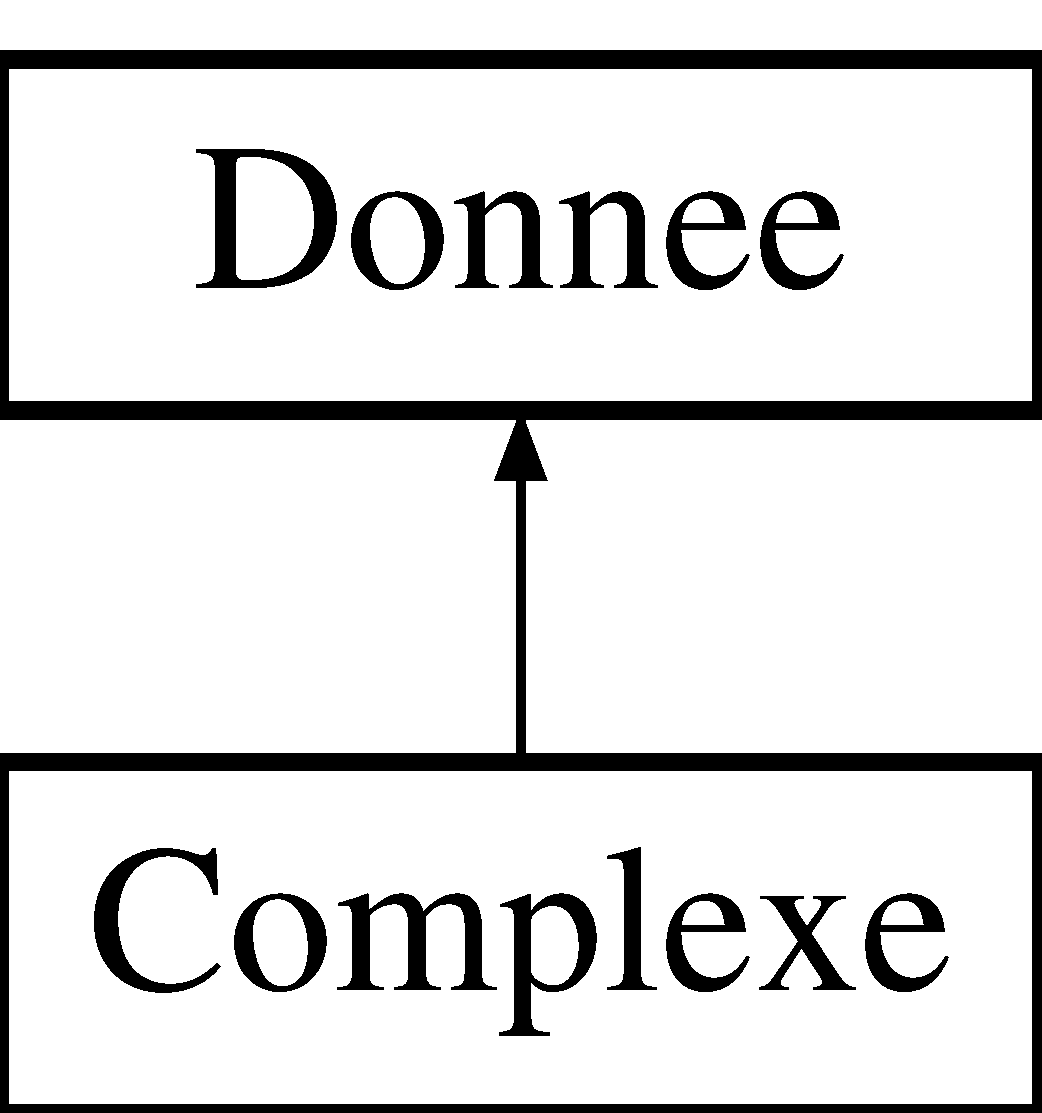
\includegraphics[height=2.000000cm]{class_complexe}
\end{center}
\end{figure}
\subsection*{Public Member Functions}
\begin{DoxyCompactItemize}
\item 
\hyperlink{class_complexe_a3e6bebaadf5b74659cf6b4eabd581733}{Complexe} (const \hyperlink{class_donnee}{Donnee} $\ast$donnee\-Depart, int type\-Souhaite)
\begin{DoxyCompactList}\small\item\em Constructeur de \hyperlink{class_complexe}{Complexe} � partir d'une \hyperlink{class_donnee}{Donnee} initiale et selon un type souhait� \end{DoxyCompactList}\item 
\hyperlink{class_complexe_a161e05ff800f7c550e014459d11948ce}{Complexe} (\hyperlink{class_constante}{Constante} $\ast$D1=0, \hyperlink{class_constante}{Constante} $\ast$D2=0)
\begin{DoxyCompactList}\small\item\em Constructeur de \hyperlink{class_complexe}{Complexe} � partir de 2 pointeurs de Constantes. \end{DoxyCompactList}\item 
\hyperlink{class_complexe_a185ea35403490637aab61d1422f4bae1}{Complexe} (const \hyperlink{class_complexe}{Complexe} $\ast$a\-Complexe)
\begin{DoxyCompactList}\small\item\em Constructeur de \hyperlink{class_complexe}{Complexe} � partir d'un pointeur vers \hyperlink{class_complexe}{Complexe}. \end{DoxyCompactList}\item 
\hyperlink{class_complexe_a4330a88cb943a61238dde5f8f58ca8a5}{Complexe} (const \hyperlink{class_entier}{Entier} $\ast$a\-Entier)
\begin{DoxyCompactList}\small\item\em Constructeur de \hyperlink{class_complexe}{Complexe} � partir d'un pointeur vers \hyperlink{class_entier}{Entier}. \end{DoxyCompactList}\item 
\hyperlink{class_complexe_a2ad5ef5f7aa244603ff6fdd13bb8cd1c}{Complexe} (const \hyperlink{class_reel}{Reel} $\ast$a\-Reel)
\begin{DoxyCompactList}\small\item\em Constructeur de \hyperlink{class_complexe}{Complexe} � partir d'un pointeur vers \hyperlink{class_reel}{Reel}. \end{DoxyCompactList}\item 
\hyperlink{class_complexe_abcd436bc78e96ed80dac1c9dbe764e6c}{Complexe} (const \hyperlink{class_rationnel}{Rationnel} $\ast$a\-Rationnel)
\begin{DoxyCompactList}\small\item\em Constructeur de \hyperlink{class_complexe}{Complexe} � partir d'un pointeur vers \hyperlink{class_rationnel}{Rationnel}. \end{DoxyCompactList}\item 
\hyperlink{class_complexe_a8ae4f6c56823f3dd6522883b3dbcf059}{Complexe} (const Q\-String \&s)
\begin{DoxyCompactList}\small\item\em Constructeur de \hyperlink{class_complexe}{Complexe} � partir d'une Q\-String. \end{DoxyCompactList}\item 
\hypertarget{class_complexe_ac92996231047d39d40e11384bb9311b6}{\hyperlink{class_complexe_ac92996231047d39d40e11384bb9311b6}{$\sim$\-Complexe} ()}\label{class_complexe_ac92996231047d39d40e11384bb9311b6}

\begin{DoxyCompactList}\small\item\em Destructeur. \end{DoxyCompactList}\item 
virtual Q\-String \hyperlink{class_complexe_ab58e8f5243f79c4a9053a100e8b418f5}{to\-Q\-String} () const 
\begin{DoxyCompactList}\small\item\em M�thode permettant d'obtenir l'objet sous la forme d'une Qstring. \end{DoxyCompactList}\item 
\hyperlink{class_constante}{Constante} $\ast$ \hyperlink{class_complexe_ad557f0b0553a4210da67dd906b35efa7}{get\-P\-Re} () const 
\begin{DoxyCompactList}\small\item\em Accesseur � la partie r�elle. \end{DoxyCompactList}\item 
\hyperlink{class_constante}{Constante} $\ast$ \hyperlink{class_complexe_af1e92ffcc7aaf7bbb118b2406410b03e}{get\-P\-Im} () const 
\begin{DoxyCompactList}\small\item\em Accesseur � la partie imaginaire. \end{DoxyCompactList}\item 
\hyperlink{class_donnee}{Donnee} $\ast$ \hyperlink{class_complexe_a6ebc6f1b73086fdfe5807ed157cd219b}{conj} ()
\begin{DoxyCompactList}\small\item\em Construit le conjugu� du \hyperlink{class_complexe}{Complexe}. \end{DoxyCompactList}\item 
\hyperlink{class_donnee}{Donnee} $\ast$ \hyperlink{class_complexe_ad4472b5e5eb0cc7ecd7ae26e20672f4a}{operator+} (\hyperlink{class_donnee}{Donnee} $\ast$t)
\begin{DoxyCompactList}\small\item\em Operateur +. \end{DoxyCompactList}\item 
\hyperlink{class_donnee}{Donnee} $\ast$ \hyperlink{class_complexe_a67686b9d236ff43809a4fd82197abadd}{operator/} (\hyperlink{class_donnee}{Donnee} $\ast$t)
\begin{DoxyCompactList}\small\item\em Operateur /. \end{DoxyCompactList}\item 
\hyperlink{class_donnee}{Donnee} $\ast$ \hyperlink{class_complexe_a620f8ada80203699ee56323c6e30477b}{operator$\ast$} (\hyperlink{class_donnee}{Donnee} $\ast$t)
\begin{DoxyCompactList}\small\item\em Operateur $\ast$. \end{DoxyCompactList}\item 
\hyperlink{class_donnee}{Donnee} $\ast$ \hyperlink{class_complexe_acee489797c36716c369ec81f368adf11}{operator-\/} (\hyperlink{class_donnee}{Donnee} $\ast$t)
\begin{DoxyCompactList}\small\item\em Operateur -\/. \end{DoxyCompactList}\item 
\hyperlink{class_complexe}{Complexe} $\ast$ \hyperlink{class_complexe_afa604ee69a629d0244fd1f60640e76f1}{sign} ()
\begin{DoxyCompactList}\small\item\em Retourne un \hyperlink{class_complexe}{Complexe} ayant les memes valeurs mais avec le signe invers� \end{DoxyCompactList}\item 
virtual \hyperlink{class_donnee}{Donnee} $\ast$ \hyperlink{class_complexe_a0ffebc558e7de92e447c12e0878d2216}{puissance} (\hyperlink{class_donnee}{Donnee} $\ast$t)
\begin{DoxyCompactList}\small\item\em puissance \end{DoxyCompactList}\item 
virtual \hyperlink{class_donnee}{Donnee} $\ast$ \hyperlink{class_complexe_a51e608468a6d5772ccf83b2c1c3dae00}{mod} (\hyperlink{class_donnee}{Donnee} $\ast$t)
\begin{DoxyCompactList}\small\item\em mod \end{DoxyCompactList}\item 
virtual \hyperlink{class_donnee}{Donnee} $\ast$ \hyperlink{class_complexe_a28ef9488dd8b7cfdf3693933f05c7602}{my\-Sin} (int type\-Angle)
\begin{DoxyCompactList}\small\item\em my\-Sin \end{DoxyCompactList}\item 
virtual \hyperlink{class_donnee}{Donnee} $\ast$ \hyperlink{class_complexe_a8d3b7489a1d26778436bd618fd068e9d}{my\-Cos} (int type\-Angle)
\begin{DoxyCompactList}\small\item\em my\-Cos \end{DoxyCompactList}\item 
virtual \hyperlink{class_donnee}{Donnee} $\ast$ \hyperlink{class_complexe_aa983852c4813b6dfc7d63f3f7e24376e}{my\-Tan} (int type\-Angle)
\begin{DoxyCompactList}\small\item\em my\-Tan \end{DoxyCompactList}\item 
virtual \hyperlink{class_donnee}{Donnee} $\ast$ \hyperlink{class_complexe_acaa8fd8e9e1875586de3a5f6cf878e26}{my\-Sinh} (int type\-Angle)
\begin{DoxyCompactList}\small\item\em my\-Sinh \end{DoxyCompactList}\item 
virtual \hyperlink{class_donnee}{Donnee} $\ast$ \hyperlink{class_complexe_ac45496aad709a8b088661fee205d7ec7}{my\-Cosh} (int type\-Angle)
\begin{DoxyCompactList}\small\item\em my\-Cosh \end{DoxyCompactList}\item 
virtual \hyperlink{class_donnee}{Donnee} $\ast$ \hyperlink{class_complexe_a524e5444c902beeb324a2769e6b92fff}{my\-Tanh} (int type\-Angle)
\begin{DoxyCompactList}\small\item\em my\-Tanh \end{DoxyCompactList}\item 
virtual \hyperlink{class_donnee}{Donnee} $\ast$ \hyperlink{class_complexe_aeb9ab54d908c6fbe602d29ac21c52b16}{my\-Ln} ()
\begin{DoxyCompactList}\small\item\em my\-Ln \end{DoxyCompactList}\item 
virtual \hyperlink{class_donnee}{Donnee} $\ast$ \hyperlink{class_complexe_a3582455cbfc8c3c5a066711f75b0cc63}{my\-Log} ()
\begin{DoxyCompactList}\small\item\em my\-Log \end{DoxyCompactList}\item 
virtual \hyperlink{class_donnee}{Donnee} $\ast$ \hyperlink{class_complexe_a020741c51dc93a684739dcbadd18b0f6}{my\-Inv} ()
\begin{DoxyCompactList}\small\item\em my\-Inv \end{DoxyCompactList}\item 
virtual \hyperlink{class_donnee}{Donnee} $\ast$ \hyperlink{class_complexe_a2c36d7a1ce2b853d371f4f3ea6248a95}{my\-Sqrt} ()
\begin{DoxyCompactList}\small\item\em my\-Sqrt \end{DoxyCompactList}\item 
virtual \hyperlink{class_donnee}{Donnee} $\ast$ \hyperlink{class_complexe_aba5e89ace5cb5f41923926a69dd6e240}{my\-Sqr} ()
\begin{DoxyCompactList}\small\item\em my\-Sqr \end{DoxyCompactList}\item 
virtual \hyperlink{class_donnee}{Donnee} $\ast$ \hyperlink{class_complexe_a8d8487e7073e297e0abba4913baaa1c8}{my\-Cube} ()
\begin{DoxyCompactList}\small\item\em my\-Cube \end{DoxyCompactList}\item 
virtual \hyperlink{class_donnee}{Donnee} $\ast$ \hyperlink{class_complexe_a8ad7815a2c7d75f51bc3aa19d99062eb}{my\-Fact} ()
\begin{DoxyCompactList}\small\item\em my\-Fact \end{DoxyCompactList}\item 
bool \hyperlink{class_complexe_a37fff7862b069bb790a439e968d820bf}{is\-Zero} ()
\begin{DoxyCompactList}\small\item\em is\-Zero \end{DoxyCompactList}\item 
bool \hyperlink{class_complexe_a8946f7fadb114404aaef719bb1c17f1b}{is\-Neg} ()
\begin{DoxyCompactList}\small\item\em is\-Neg \end{DoxyCompactList}\end{DoxyCompactItemize}
\subsection*{Additional Inherited Members}


\subsection{Detailed Description}
Classe mod�lisant les complexes. Elle h�rite de \hyperlink{class_donnee}{Donnee}. 

\begin{DoxyAuthor}{Author}
Letellier/\-Yassine
\end{DoxyAuthor}
Pour fonctionner cette classe encapsule deux Constantes \-: sa partie r�elle et sa partie imaginaire. Tous les op�rateurs sont �galements red�finis. 

\subsection{Constructor \& Destructor Documentation}
\hypertarget{class_complexe_a3e6bebaadf5b74659cf6b4eabd581733}{\index{Complexe@{Complexe}!Complexe@{Complexe}}
\index{Complexe@{Complexe}!Complexe@{Complexe}}
\subsubsection[{Complexe}]{\setlength{\rightskip}{0pt plus 5cm}Complexe\-::\-Complexe (
\begin{DoxyParamCaption}
\item[{const {\bf Donnee} $\ast$}]{donnee\-Depart, }
\item[{int}]{type\-Souhaite}
\end{DoxyParamCaption}
)}}\label{class_complexe_a3e6bebaadf5b74659cf6b4eabd581733}


Constructeur de \hyperlink{class_complexe}{Complexe} � partir d'une \hyperlink{class_donnee}{Donnee} initiale et selon un type souhait� 


\begin{DoxyParams}{Parameters}
{\em donnee\-Depart} & Pointeur vers la \hyperlink{class_donnee}{Donnee} contenant les valeurs nous int�ressant \\
\hline
{\em type\-Souhaite} & Descripteur du type qui formatera les attributs de ce \hyperlink{class_complexe}{Complexe} \\
\hline
\end{DoxyParams}
\begin{DoxyReturn}{Returns}
Elle retourne le \hyperlink{class_complexe}{Complexe} construit. 
\end{DoxyReturn}
\hypertarget{class_complexe_a161e05ff800f7c550e014459d11948ce}{\index{Complexe@{Complexe}!Complexe@{Complexe}}
\index{Complexe@{Complexe}!Complexe@{Complexe}}
\subsubsection[{Complexe}]{\setlength{\rightskip}{0pt plus 5cm}Complexe\-::\-Complexe (
\begin{DoxyParamCaption}
\item[{{\bf Constante} $\ast$}]{D1 = {\ttfamily 0}, }
\item[{{\bf Constante} $\ast$}]{D2 = {\ttfamily 0}}
\end{DoxyParamCaption}
)\hspace{0.3cm}{\ttfamily [inline]}}}\label{class_complexe_a161e05ff800f7c550e014459d11948ce}


Constructeur de \hyperlink{class_complexe}{Complexe} � partir de 2 pointeurs de Constantes. 


\begin{DoxyParams}{Parameters}
{\em D1} & \hyperlink{class_constante}{Constante} initialisant la partie r�elle \\
\hline
{\em D2} & \hyperlink{class_constante}{Constante} initialisant la partie imaginaire \\
\hline
\end{DoxyParams}
\begin{DoxyReturn}{Returns}
Elle retourne le \hyperlink{class_complexe}{Complexe} construit. 
\end{DoxyReturn}
\hypertarget{class_complexe_a185ea35403490637aab61d1422f4bae1}{\index{Complexe@{Complexe}!Complexe@{Complexe}}
\index{Complexe@{Complexe}!Complexe@{Complexe}}
\subsubsection[{Complexe}]{\setlength{\rightskip}{0pt plus 5cm}Complexe\-::\-Complexe (
\begin{DoxyParamCaption}
\item[{const {\bf Complexe} $\ast$}]{a\-Complexe}
\end{DoxyParamCaption}
)}}\label{class_complexe_a185ea35403490637aab61d1422f4bae1}


Constructeur de \hyperlink{class_complexe}{Complexe} � partir d'un pointeur vers \hyperlink{class_complexe}{Complexe}. 


\begin{DoxyParams}{Parameters}
{\em a\-Complexe} & Pointeur vers un \hyperlink{class_complexe}{Complexe} \\
\hline
\end{DoxyParams}
\begin{DoxyReturn}{Returns}
Elle retourne le \hyperlink{class_complexe}{Complexe} construit. 
\end{DoxyReturn}
\hypertarget{class_complexe_a4330a88cb943a61238dde5f8f58ca8a5}{\index{Complexe@{Complexe}!Complexe@{Complexe}}
\index{Complexe@{Complexe}!Complexe@{Complexe}}
\subsubsection[{Complexe}]{\setlength{\rightskip}{0pt plus 5cm}Complexe\-::\-Complexe (
\begin{DoxyParamCaption}
\item[{const {\bf Entier} $\ast$}]{a\-Entier}
\end{DoxyParamCaption}
)}}\label{class_complexe_a4330a88cb943a61238dde5f8f58ca8a5}


Constructeur de \hyperlink{class_complexe}{Complexe} � partir d'un pointeur vers \hyperlink{class_entier}{Entier}. 


\begin{DoxyParams}{Parameters}
{\em a\-Entier} & Pointeur vers un \hyperlink{class_entier}{Entier} \\
\hline
\end{DoxyParams}
\begin{DoxyReturn}{Returns}
Elle retourne le \hyperlink{class_complexe}{Complexe} construit. 
\end{DoxyReturn}
\hypertarget{class_complexe_a2ad5ef5f7aa244603ff6fdd13bb8cd1c}{\index{Complexe@{Complexe}!Complexe@{Complexe}}
\index{Complexe@{Complexe}!Complexe@{Complexe}}
\subsubsection[{Complexe}]{\setlength{\rightskip}{0pt plus 5cm}Complexe\-::\-Complexe (
\begin{DoxyParamCaption}
\item[{const {\bf Reel} $\ast$}]{a\-Reel}
\end{DoxyParamCaption}
)}}\label{class_complexe_a2ad5ef5f7aa244603ff6fdd13bb8cd1c}


Constructeur de \hyperlink{class_complexe}{Complexe} � partir d'un pointeur vers \hyperlink{class_reel}{Reel}. 


\begin{DoxyParams}{Parameters}
{\em a\-Reel} & Pointeur vers un \hyperlink{class_reel}{Reel} \\
\hline
\end{DoxyParams}
\begin{DoxyReturn}{Returns}
Elle retourne le \hyperlink{class_complexe}{Complexe} construit. 
\end{DoxyReturn}
\hypertarget{class_complexe_abcd436bc78e96ed80dac1c9dbe764e6c}{\index{Complexe@{Complexe}!Complexe@{Complexe}}
\index{Complexe@{Complexe}!Complexe@{Complexe}}
\subsubsection[{Complexe}]{\setlength{\rightskip}{0pt plus 5cm}Complexe\-::\-Complexe (
\begin{DoxyParamCaption}
\item[{const {\bf Rationnel} $\ast$}]{a\-Rationnel}
\end{DoxyParamCaption}
)}}\label{class_complexe_abcd436bc78e96ed80dac1c9dbe764e6c}


Constructeur de \hyperlink{class_complexe}{Complexe} � partir d'un pointeur vers \hyperlink{class_rationnel}{Rationnel}. 


\begin{DoxyParams}{Parameters}
{\em a\-Rationnel} & Pointeur vers un \hyperlink{class_rationnel}{Rationnel} \\
\hline
\end{DoxyParams}
\begin{DoxyReturn}{Returns}
Elle retourne le \hyperlink{class_complexe}{Complexe} construit. 
\end{DoxyReturn}
\hypertarget{class_complexe_a8ae4f6c56823f3dd6522883b3dbcf059}{\index{Complexe@{Complexe}!Complexe@{Complexe}}
\index{Complexe@{Complexe}!Complexe@{Complexe}}
\subsubsection[{Complexe}]{\setlength{\rightskip}{0pt plus 5cm}Complexe\-::\-Complexe (
\begin{DoxyParamCaption}
\item[{const Q\-String \&}]{s}
\end{DoxyParamCaption}
)}}\label{class_complexe_a8ae4f6c56823f3dd6522883b3dbcf059}


Constructeur de \hyperlink{class_complexe}{Complexe} � partir d'une Q\-String. 


\begin{DoxyParams}{Parameters}
{\em s} & Q\-String de la forme reel\$imaginaire \\
\hline
\end{DoxyParams}
\begin{DoxyReturn}{Returns}
Elle retourne le \hyperlink{class_complexe}{Complexe} construit. 
\end{DoxyReturn}


\subsection{Member Function Documentation}
\hypertarget{class_complexe_a6ebc6f1b73086fdfe5807ed157cd219b}{\index{Complexe@{Complexe}!conj@{conj}}
\index{conj@{conj}!Complexe@{Complexe}}
\subsubsection[{conj}]{\setlength{\rightskip}{0pt plus 5cm}{\bf Donnee} $\ast$ Complexe\-::conj (
\begin{DoxyParamCaption}
{}
\end{DoxyParamCaption}
)}}\label{class_complexe_a6ebc6f1b73086fdfe5807ed157cd219b}


Construit le conjugu� du \hyperlink{class_complexe}{Complexe}. 

\begin{DoxyReturn}{Returns}
Retourne un pointeur vers ce nouveau \hyperlink{class_complexe}{Complexe}. 
\end{DoxyReturn}
\hypertarget{class_complexe_af1e92ffcc7aaf7bbb118b2406410b03e}{\index{Complexe@{Complexe}!get\-P\-Im@{get\-P\-Im}}
\index{get\-P\-Im@{get\-P\-Im}!Complexe@{Complexe}}
\subsubsection[{get\-P\-Im}]{\setlength{\rightskip}{0pt plus 5cm}{\bf Constante}$\ast$ Complexe\-::get\-P\-Im (
\begin{DoxyParamCaption}
{}
\end{DoxyParamCaption}
) const\hspace{0.3cm}{\ttfamily [inline]}}}\label{class_complexe_af1e92ffcc7aaf7bbb118b2406410b03e}


Accesseur � la partie imaginaire. 

\begin{DoxyReturn}{Returns}
Retourne l'attribut-\/pointeur vers la partie imaginaire du \hyperlink{class_complexe}{Complexe}. 
\end{DoxyReturn}
\hypertarget{class_complexe_ad557f0b0553a4210da67dd906b35efa7}{\index{Complexe@{Complexe}!get\-P\-Re@{get\-P\-Re}}
\index{get\-P\-Re@{get\-P\-Re}!Complexe@{Complexe}}
\subsubsection[{get\-P\-Re}]{\setlength{\rightskip}{0pt plus 5cm}{\bf Constante}$\ast$ Complexe\-::get\-P\-Re (
\begin{DoxyParamCaption}
{}
\end{DoxyParamCaption}
) const\hspace{0.3cm}{\ttfamily [inline]}}}\label{class_complexe_ad557f0b0553a4210da67dd906b35efa7}


Accesseur � la partie r�elle. 

\begin{DoxyReturn}{Returns}
Retourne l'attribut-\/pointeur vers la partie r�elle du \hyperlink{class_complexe}{Complexe}. 
\end{DoxyReturn}
\hypertarget{class_complexe_a8946f7fadb114404aaef719bb1c17f1b}{\index{Complexe@{Complexe}!is\-Neg@{is\-Neg}}
\index{is\-Neg@{is\-Neg}!Complexe@{Complexe}}
\subsubsection[{is\-Neg}]{\setlength{\rightskip}{0pt plus 5cm}bool Complexe\-::is\-Neg (
\begin{DoxyParamCaption}
{}
\end{DoxyParamCaption}
)\hspace{0.3cm}{\ttfamily [inline]}, {\ttfamily [virtual]}}}\label{class_complexe_a8946f7fadb114404aaef719bb1c17f1b}


is\-Neg 

Mathode permettant de savoir si la \hyperlink{class_donnee}{Donnee} est inferieure ou egale � 0 \begin{DoxyReturn}{Returns}
bool true si la \hyperlink{class_donnee}{Donnee} est inferieur ou egale � 0 
\end{DoxyReturn}


Implements \hyperlink{class_donnee_a0efb324f0c2e0682b971c3692c46e7c3}{Donnee}.

\hypertarget{class_complexe_a37fff7862b069bb790a439e968d820bf}{\index{Complexe@{Complexe}!is\-Zero@{is\-Zero}}
\index{is\-Zero@{is\-Zero}!Complexe@{Complexe}}
\subsubsection[{is\-Zero}]{\setlength{\rightskip}{0pt plus 5cm}bool Complexe\-::is\-Zero (
\begin{DoxyParamCaption}
{}
\end{DoxyParamCaption}
)\hspace{0.3cm}{\ttfamily [inline]}, {\ttfamily [virtual]}}}\label{class_complexe_a37fff7862b069bb790a439e968d820bf}


is\-Zero 

Mathode permettant de savoir si la \hyperlink{class_donnee}{Donnee} est egale � 0 \begin{DoxyReturn}{Returns}
bool true si la \hyperlink{class_donnee}{Donnee} est egale � 0 
\end{DoxyReturn}


Implements \hyperlink{class_donnee_aad251e4148c791719d7d7bff18680611}{Donnee}.

\hypertarget{class_complexe_a51e608468a6d5772ccf83b2c1c3dae00}{\index{Complexe@{Complexe}!mod@{mod}}
\index{mod@{mod}!Complexe@{Complexe}}
\subsubsection[{mod}]{\setlength{\rightskip}{0pt plus 5cm}virtual {\bf Donnee}$\ast$ Complexe\-::mod (
\begin{DoxyParamCaption}
\item[{{\bf Donnee} $\ast$}]{t}
\end{DoxyParamCaption}
)\hspace{0.3cm}{\ttfamily [inline]}, {\ttfamily [virtual]}}}\label{class_complexe_a51e608468a6d5772ccf83b2c1c3dae00}


mod 

Implementation de l'operateur binaire modulo (methode virtuelle dans la classe mere) 
\begin{DoxyParams}{Parameters}
{\em Donnee$\ast$,\-:} & Pointeur sur une donnee \\
\hline
\end{DoxyParams}
\begin{DoxyReturn}{Returns}
Pointeur sur donnee, resultat de l'operation 
\end{DoxyReturn}


Implements \hyperlink{class_donnee}{Donnee}.

\hypertarget{class_complexe_a8d3b7489a1d26778436bd618fd068e9d}{\index{Complexe@{Complexe}!my\-Cos@{my\-Cos}}
\index{my\-Cos@{my\-Cos}!Complexe@{Complexe}}
\subsubsection[{my\-Cos}]{\setlength{\rightskip}{0pt plus 5cm}virtual {\bf Donnee}$\ast$ Complexe\-::my\-Cos (
\begin{DoxyParamCaption}
\item[{int}]{type\-Angle}
\end{DoxyParamCaption}
)\hspace{0.3cm}{\ttfamily [inline]}, {\ttfamily [virtual]}}}\label{class_complexe_a8d3b7489a1d26778436bd618fd068e9d}


my\-Cos 

Implementation de l'operateur unaire cosinus (methode virtuelle dans la classe mere) 
\begin{DoxyParams}{Parameters}
{\em type\-Angle} & \-: entier, 0 si utilisation des degres, 1 si utilisation des radians \\
\hline
\end{DoxyParams}
\begin{DoxyReturn}{Returns}
Pointeur sur donnee, resultat de l'operation 
\end{DoxyReturn}


Implements \hyperlink{class_donnee}{Donnee}.

\hypertarget{class_complexe_ac45496aad709a8b088661fee205d7ec7}{\index{Complexe@{Complexe}!my\-Cosh@{my\-Cosh}}
\index{my\-Cosh@{my\-Cosh}!Complexe@{Complexe}}
\subsubsection[{my\-Cosh}]{\setlength{\rightskip}{0pt plus 5cm}virtual {\bf Donnee}$\ast$ Complexe\-::my\-Cosh (
\begin{DoxyParamCaption}
\item[{int}]{type\-Angle}
\end{DoxyParamCaption}
)\hspace{0.3cm}{\ttfamily [inline]}, {\ttfamily [virtual]}}}\label{class_complexe_ac45496aad709a8b088661fee205d7ec7}


my\-Cosh 

Implementation de l'operateur unaire cosinush (methode virtuelle dans la classe mere) 
\begin{DoxyParams}{Parameters}
{\em type\-Angle} & \-: entier, 0 si utilisation des degres, 1 si utilisation des radians \\
\hline
\end{DoxyParams}
\begin{DoxyReturn}{Returns}
Pointeur sur donnee, resultat de l'operation 
\end{DoxyReturn}


Implements \hyperlink{class_donnee}{Donnee}.

\hypertarget{class_complexe_a8d8487e7073e297e0abba4913baaa1c8}{\index{Complexe@{Complexe}!my\-Cube@{my\-Cube}}
\index{my\-Cube@{my\-Cube}!Complexe@{Complexe}}
\subsubsection[{my\-Cube}]{\setlength{\rightskip}{0pt plus 5cm}{\bf Donnee} $\ast$ Complexe\-::my\-Cube (
\begin{DoxyParamCaption}
{}
\end{DoxyParamCaption}
)\hspace{0.3cm}{\ttfamily [virtual]}}}\label{class_complexe_a8d8487e7073e297e0abba4913baaa1c8}


my\-Cube 

Implementation de l'operateur unaire Cube (methode virtuelle dans la classe mere) \begin{DoxyReturn}{Returns}
Pointeur sur donnee, resultat de l'operation 
\end{DoxyReturn}


Implements \hyperlink{class_donnee}{Donnee}.

\hypertarget{class_complexe_a8ad7815a2c7d75f51bc3aa19d99062eb}{\index{Complexe@{Complexe}!my\-Fact@{my\-Fact}}
\index{my\-Fact@{my\-Fact}!Complexe@{Complexe}}
\subsubsection[{my\-Fact}]{\setlength{\rightskip}{0pt plus 5cm}virtual {\bf Donnee}$\ast$ Complexe\-::my\-Fact (
\begin{DoxyParamCaption}
{}
\end{DoxyParamCaption}
)\hspace{0.3cm}{\ttfamily [inline]}, {\ttfamily [virtual]}}}\label{class_complexe_a8ad7815a2c7d75f51bc3aa19d99062eb}


my\-Fact 

Implementation de l'operateur unaire fact (methode virtuelle dans la classe mere) \begin{DoxyReturn}{Returns}
Pointeur sur donnee, resultat de l'operation 
\end{DoxyReturn}


Implements \hyperlink{class_donnee}{Donnee}.

\hypertarget{class_complexe_a020741c51dc93a684739dcbadd18b0f6}{\index{Complexe@{Complexe}!my\-Inv@{my\-Inv}}
\index{my\-Inv@{my\-Inv}!Complexe@{Complexe}}
\subsubsection[{my\-Inv}]{\setlength{\rightskip}{0pt plus 5cm}virtual {\bf Donnee}$\ast$ Complexe\-::my\-Inv (
\begin{DoxyParamCaption}
{}
\end{DoxyParamCaption}
)\hspace{0.3cm}{\ttfamily [inline]}, {\ttfamily [virtual]}}}\label{class_complexe_a020741c51dc93a684739dcbadd18b0f6}


my\-Inv 

Implementation de l'operateur unaire inv (methode virtuelle dans la classe mere) \begin{DoxyReturn}{Returns}
Pointeur sur donnee, resultat de l'operation 
\end{DoxyReturn}


Implements \hyperlink{class_donnee}{Donnee}.

\hypertarget{class_complexe_aeb9ab54d908c6fbe602d29ac21c52b16}{\index{Complexe@{Complexe}!my\-Ln@{my\-Ln}}
\index{my\-Ln@{my\-Ln}!Complexe@{Complexe}}
\subsubsection[{my\-Ln}]{\setlength{\rightskip}{0pt plus 5cm}virtual {\bf Donnee}$\ast$ Complexe\-::my\-Ln (
\begin{DoxyParamCaption}
{}
\end{DoxyParamCaption}
)\hspace{0.3cm}{\ttfamily [inline]}, {\ttfamily [virtual]}}}\label{class_complexe_aeb9ab54d908c6fbe602d29ac21c52b16}


my\-Ln 

Implementation de l'operateur unaire ln (methode virtuelle dans la classe mere) \begin{DoxyReturn}{Returns}
Pointeur sur donnee, resultat de l'operation 
\end{DoxyReturn}


Implements \hyperlink{class_donnee}{Donnee}.

\hypertarget{class_complexe_a3582455cbfc8c3c5a066711f75b0cc63}{\index{Complexe@{Complexe}!my\-Log@{my\-Log}}
\index{my\-Log@{my\-Log}!Complexe@{Complexe}}
\subsubsection[{my\-Log}]{\setlength{\rightskip}{0pt plus 5cm}virtual {\bf Donnee}$\ast$ Complexe\-::my\-Log (
\begin{DoxyParamCaption}
{}
\end{DoxyParamCaption}
)\hspace{0.3cm}{\ttfamily [inline]}, {\ttfamily [virtual]}}}\label{class_complexe_a3582455cbfc8c3c5a066711f75b0cc63}


my\-Log 

Implementation de l'operateur unaire log (methode virtuelle dans la classe mere) \begin{DoxyReturn}{Returns}
Pointeur sur donnee, resultat de l'operation 
\end{DoxyReturn}


Implements \hyperlink{class_donnee}{Donnee}.

\hypertarget{class_complexe_a28ef9488dd8b7cfdf3693933f05c7602}{\index{Complexe@{Complexe}!my\-Sin@{my\-Sin}}
\index{my\-Sin@{my\-Sin}!Complexe@{Complexe}}
\subsubsection[{my\-Sin}]{\setlength{\rightskip}{0pt plus 5cm}virtual {\bf Donnee}$\ast$ Complexe\-::my\-Sin (
\begin{DoxyParamCaption}
\item[{int}]{type\-Angle}
\end{DoxyParamCaption}
)\hspace{0.3cm}{\ttfamily [inline]}, {\ttfamily [virtual]}}}\label{class_complexe_a28ef9488dd8b7cfdf3693933f05c7602}


my\-Sin 

Implementation de l'operateur unaire sinus (methode virtuelle dans la classe mere) 
\begin{DoxyParams}{Parameters}
{\em type\-Angle} & \-: entier, 0 si utilisation des degres, 1 si utilisation des radians \\
\hline
\end{DoxyParams}
\begin{DoxyReturn}{Returns}
Pointeur sur donnee, resultat de l'operation 
\end{DoxyReturn}


Implements \hyperlink{class_donnee}{Donnee}.

\hypertarget{class_complexe_acaa8fd8e9e1875586de3a5f6cf878e26}{\index{Complexe@{Complexe}!my\-Sinh@{my\-Sinh}}
\index{my\-Sinh@{my\-Sinh}!Complexe@{Complexe}}
\subsubsection[{my\-Sinh}]{\setlength{\rightskip}{0pt plus 5cm}virtual {\bf Donnee}$\ast$ Complexe\-::my\-Sinh (
\begin{DoxyParamCaption}
\item[{int}]{type\-Angle}
\end{DoxyParamCaption}
)\hspace{0.3cm}{\ttfamily [inline]}, {\ttfamily [virtual]}}}\label{class_complexe_acaa8fd8e9e1875586de3a5f6cf878e26}


my\-Sinh 

Implementation de l'operateur unaire sinush (methode virtuelle dans la classe mere) 
\begin{DoxyParams}{Parameters}
{\em type\-Angle} & \-: entier, 0 si utilisation des degres, 1 si utilisation des radians \\
\hline
\end{DoxyParams}
\begin{DoxyReturn}{Returns}
Pointeur sur donnee, resultat de l'operation 
\end{DoxyReturn}


Implements \hyperlink{class_donnee}{Donnee}.

\hypertarget{class_complexe_aba5e89ace5cb5f41923926a69dd6e240}{\index{Complexe@{Complexe}!my\-Sqr@{my\-Sqr}}
\index{my\-Sqr@{my\-Sqr}!Complexe@{Complexe}}
\subsubsection[{my\-Sqr}]{\setlength{\rightskip}{0pt plus 5cm}{\bf Donnee} $\ast$ Complexe\-::my\-Sqr (
\begin{DoxyParamCaption}
{}
\end{DoxyParamCaption}
)\hspace{0.3cm}{\ttfamily [virtual]}}}\label{class_complexe_aba5e89ace5cb5f41923926a69dd6e240}


my\-Sqr 

Implementation de l'operateur unaire sqr (methode virtuelle dans la classe mere) \begin{DoxyReturn}{Returns}
Pointeur sur donnee, resultat de l'operation 
\end{DoxyReturn}


Implements \hyperlink{class_donnee}{Donnee}.

\hypertarget{class_complexe_a2c36d7a1ce2b853d371f4f3ea6248a95}{\index{Complexe@{Complexe}!my\-Sqrt@{my\-Sqrt}}
\index{my\-Sqrt@{my\-Sqrt}!Complexe@{Complexe}}
\subsubsection[{my\-Sqrt}]{\setlength{\rightskip}{0pt plus 5cm}virtual {\bf Donnee}$\ast$ Complexe\-::my\-Sqrt (
\begin{DoxyParamCaption}
{}
\end{DoxyParamCaption}
)\hspace{0.3cm}{\ttfamily [inline]}, {\ttfamily [virtual]}}}\label{class_complexe_a2c36d7a1ce2b853d371f4f3ea6248a95}


my\-Sqrt 

Implementation de l'operateur unaire sqrt (methode virtuelle dans la classe mere) \begin{DoxyReturn}{Returns}
Pointeur sur donnee, resultat de l'operation 
\end{DoxyReturn}


Implements \hyperlink{class_donnee}{Donnee}.

\hypertarget{class_complexe_aa983852c4813b6dfc7d63f3f7e24376e}{\index{Complexe@{Complexe}!my\-Tan@{my\-Tan}}
\index{my\-Tan@{my\-Tan}!Complexe@{Complexe}}
\subsubsection[{my\-Tan}]{\setlength{\rightskip}{0pt plus 5cm}virtual {\bf Donnee}$\ast$ Complexe\-::my\-Tan (
\begin{DoxyParamCaption}
\item[{int}]{type\-Angle}
\end{DoxyParamCaption}
)\hspace{0.3cm}{\ttfamily [inline]}, {\ttfamily [virtual]}}}\label{class_complexe_aa983852c4813b6dfc7d63f3f7e24376e}


my\-Tan 

Implementation de l'operateur unaire tangente (methode virtuelle dans la classe mere) 
\begin{DoxyParams}{Parameters}
{\em type\-Angle} & \-: entier, 0 si utilisation des degres, 1 si utilisation des radians \\
\hline
\end{DoxyParams}
\begin{DoxyReturn}{Returns}
Pointeur sur donnee, resultat de l'operation 
\end{DoxyReturn}


Implements \hyperlink{class_donnee}{Donnee}.

\hypertarget{class_complexe_a524e5444c902beeb324a2769e6b92fff}{\index{Complexe@{Complexe}!my\-Tanh@{my\-Tanh}}
\index{my\-Tanh@{my\-Tanh}!Complexe@{Complexe}}
\subsubsection[{my\-Tanh}]{\setlength{\rightskip}{0pt plus 5cm}virtual {\bf Donnee}$\ast$ Complexe\-::my\-Tanh (
\begin{DoxyParamCaption}
\item[{int}]{type\-Angle}
\end{DoxyParamCaption}
)\hspace{0.3cm}{\ttfamily [inline]}, {\ttfamily [virtual]}}}\label{class_complexe_a524e5444c902beeb324a2769e6b92fff}


my\-Tanh 

Implementation de l'operateur unaire tangenteh (methode virtuelle dans la classe mere) 
\begin{DoxyParams}{Parameters}
{\em type\-Angle} & \-: entier, 0 si utilisation des degres, 1 si utilisation des radians \\
\hline
\end{DoxyParams}
\begin{DoxyReturn}{Returns}
Pointeur sur donnee, resultat de l'operation 
\end{DoxyReturn}


Implements \hyperlink{class_donnee}{Donnee}.

\hypertarget{class_complexe_a620f8ada80203699ee56323c6e30477b}{\index{Complexe@{Complexe}!operator$\ast$@{operator$\ast$}}
\index{operator$\ast$@{operator$\ast$}!Complexe@{Complexe}}
\subsubsection[{operator$\ast$}]{\setlength{\rightskip}{0pt plus 5cm}{\bf Donnee} $\ast$ Complexe\-::operator$\ast$ (
\begin{DoxyParamCaption}
\item[{{\bf Donnee} $\ast$}]{t}
\end{DoxyParamCaption}
)\hspace{0.3cm}{\ttfamily [virtual]}}}\label{class_complexe_a620f8ada80203699ee56323c6e30477b}


Operateur $\ast$. 

Implementation de l'operateur binaire $\ast$ (methode virtuelle dans la classe mere) 
\begin{DoxyParams}{Parameters}
{\em t} & \-: Pointeur sur un type \\
\hline
\end{DoxyParams}
\begin{DoxyReturn}{Returns}
Pointeur sur type, resultat de l'operation 
\end{DoxyReturn}


Implements \hyperlink{class_donnee}{Donnee}.

\hypertarget{class_complexe_ad4472b5e5eb0cc7ecd7ae26e20672f4a}{\index{Complexe@{Complexe}!operator+@{operator+}}
\index{operator+@{operator+}!Complexe@{Complexe}}
\subsubsection[{operator+}]{\setlength{\rightskip}{0pt plus 5cm}{\bf Donnee} $\ast$ Complexe\-::operator+ (
\begin{DoxyParamCaption}
\item[{{\bf Donnee} $\ast$}]{t}
\end{DoxyParamCaption}
)\hspace{0.3cm}{\ttfamily [virtual]}}}\label{class_complexe_ad4472b5e5eb0cc7ecd7ae26e20672f4a}


Operateur +. 

Implementation de l'operateur binaire + (methode virtuelle dans la classe mere) 
\begin{DoxyParams}{Parameters}
{\em t} & \-: Pointeur sur un type \\
\hline
\end{DoxyParams}
\begin{DoxyReturn}{Returns}
Pointeur sur type, resultat de l'operation 
\end{DoxyReturn}


Implements \hyperlink{class_donnee}{Donnee}.

\hypertarget{class_complexe_acee489797c36716c369ec81f368adf11}{\index{Complexe@{Complexe}!operator-\/@{operator-\/}}
\index{operator-\/@{operator-\/}!Complexe@{Complexe}}
\subsubsection[{operator-\/}]{\setlength{\rightskip}{0pt plus 5cm}{\bf Donnee} $\ast$ Complexe\-::operator-\/ (
\begin{DoxyParamCaption}
\item[{{\bf Donnee} $\ast$}]{t}
\end{DoxyParamCaption}
)\hspace{0.3cm}{\ttfamily [virtual]}}}\label{class_complexe_acee489797c36716c369ec81f368adf11}


Operateur -\/. 

Implementation de l'operateur binaire -\/ (methode virtuelle dans la classe mere) 
\begin{DoxyParams}{Parameters}
{\em t} & \-: Pointeur sur un type \\
\hline
\end{DoxyParams}
\begin{DoxyReturn}{Returns}
Pointeur sur type, resultat de l'operation 
\end{DoxyReturn}


Implements \hyperlink{class_donnee}{Donnee}.

\hypertarget{class_complexe_a67686b9d236ff43809a4fd82197abadd}{\index{Complexe@{Complexe}!operator/@{operator/}}
\index{operator/@{operator/}!Complexe@{Complexe}}
\subsubsection[{operator/}]{\setlength{\rightskip}{0pt plus 5cm}{\bf Donnee} $\ast$ Complexe\-::operator/ (
\begin{DoxyParamCaption}
\item[{{\bf Donnee} $\ast$}]{t}
\end{DoxyParamCaption}
)\hspace{0.3cm}{\ttfamily [virtual]}}}\label{class_complexe_a67686b9d236ff43809a4fd82197abadd}


Operateur /. 

Implementation de l'operateur binaire / (methode virtuelle dans la classe mere) 
\begin{DoxyParams}{Parameters}
{\em t} & \-: Pointeur sur un type \\
\hline
\end{DoxyParams}
\begin{DoxyReturn}{Returns}
Pointeur sur type, resultat de l'operation 
\end{DoxyReturn}


Implements \hyperlink{class_donnee}{Donnee}.

\hypertarget{class_complexe_a0ffebc558e7de92e447c12e0878d2216}{\index{Complexe@{Complexe}!puissance@{puissance}}
\index{puissance@{puissance}!Complexe@{Complexe}}
\subsubsection[{puissance}]{\setlength{\rightskip}{0pt plus 5cm}virtual {\bf Donnee}$\ast$ Complexe\-::puissance (
\begin{DoxyParamCaption}
\item[{{\bf Donnee} $\ast$}]{t}
\end{DoxyParamCaption}
)\hspace{0.3cm}{\ttfamily [inline]}, {\ttfamily [virtual]}}}\label{class_complexe_a0ffebc558e7de92e447c12e0878d2216}


puissance 

Implementation de l'operateur binaire puissance (methode virtuelle dans la classe mere) 
\begin{DoxyParams}{Parameters}
{\em Donnee$\ast$,\-:} & Pointeur sur une donnee \\
\hline
\end{DoxyParams}
\begin{DoxyReturn}{Returns}
Pointeur sur donnee, resultat de l'operation 
\end{DoxyReturn}


Implements \hyperlink{class_donnee}{Donnee}.

\hypertarget{class_complexe_afa604ee69a629d0244fd1f60640e76f1}{\index{Complexe@{Complexe}!sign@{sign}}
\index{sign@{sign}!Complexe@{Complexe}}
\subsubsection[{sign}]{\setlength{\rightskip}{0pt plus 5cm}{\bf Complexe}$\ast$ Complexe\-::sign (
\begin{DoxyParamCaption}
{}
\end{DoxyParamCaption}
)\hspace{0.3cm}{\ttfamily [inline]}, {\ttfamily [virtual]}}}\label{class_complexe_afa604ee69a629d0244fd1f60640e76f1}


Retourne un \hyperlink{class_complexe}{Complexe} ayant les memes valeurs mais avec le signe invers� 

Pour fonctionner, elle utilise le constructeur \hyperlink{class_complexe_a161e05ff800f7c550e014459d11948ce}{Complexe(\-Constante$\ast$, Constante$\ast$)} \begin{DoxyVerb}   \return   Elle retourne le Complexe construit.\end{DoxyVerb}
 

Implements \hyperlink{class_donnee}{Donnee}.

\hypertarget{class_complexe_ab58e8f5243f79c4a9053a100e8b418f5}{\index{Complexe@{Complexe}!to\-Q\-String@{to\-Q\-String}}
\index{to\-Q\-String@{to\-Q\-String}!Complexe@{Complexe}}
\subsubsection[{to\-Q\-String}]{\setlength{\rightskip}{0pt plus 5cm}virtual Q\-String Complexe\-::to\-Q\-String (
\begin{DoxyParamCaption}
{}
\end{DoxyParamCaption}
) const\hspace{0.3cm}{\ttfamily [inline]}, {\ttfamily [virtual]}}}\label{class_complexe_ab58e8f5243f79c4a9053a100e8b418f5}


M�thode permettant d'obtenir l'objet sous la forme d'une Qstring. 

\begin{DoxyReturn}{Returns}
Elle retourne une Q\-String d�finissant et repr�sentant le \hyperlink{class_complexe}{Complexe}. 
\end{DoxyReturn}


Implements \hyperlink{class_donnee}{Donnee}.



The documentation for this class was generated from the following files\-:\begin{DoxyCompactItemize}
\item 
\hyperlink{complexe_8h}{complexe.\-h}\item 
complexe.\-cpp\end{DoxyCompactItemize}

\hypertarget{class_constante}{\section{Constante Class Reference}
\label{class_constante}\index{Constante@{Constante}}
}


Classe representant les types de constantes non complexes. Il s'agit d'une classe abstraite d�rivant de \hyperlink{class_donnee}{Donnee}.  




{\ttfamily \#include $<$constante.\-h$>$}

Inheritance diagram for Constante\-:\begin{figure}[H]
\begin{center}
\leavevmode
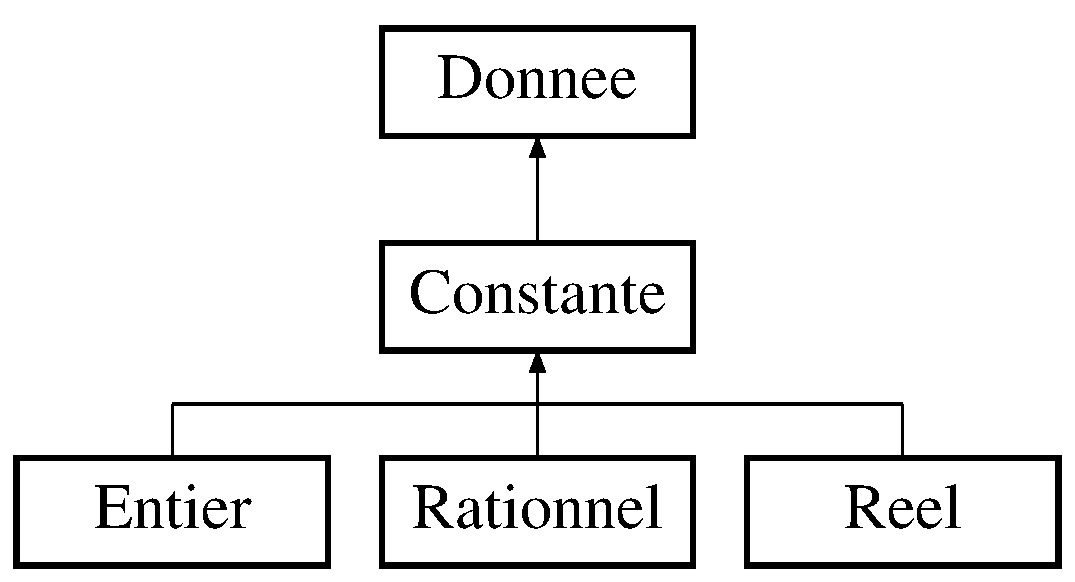
\includegraphics[height=3.000000cm]{class_constante}
\end{center}
\end{figure}
\subsection*{Public Member Functions}
\begin{DoxyCompactItemize}
\item 
\hypertarget{class_constante_ac463207a372c10cb3fe0cd999e2e2c7b}{\hyperlink{class_constante_ac463207a372c10cb3fe0cd999e2e2c7b}{Constante} ()}\label{class_constante_ac463207a372c10cb3fe0cd999e2e2c7b}

\begin{DoxyCompactList}\small\item\em Constructeur. \end{DoxyCompactList}\item 
\hypertarget{class_constante_a3d218a44f46136c5d69f04821f100953}{virtual \hyperlink{class_constante}{Constante} $\ast$ \hyperlink{class_constante_a3d218a44f46136c5d69f04821f100953}{sign} ()=0}\label{class_constante_a3d218a44f46136c5d69f04821f100953}

\begin{DoxyCompactList}\small\item\em sign M�thode virtuelle pure \end{DoxyCompactList}\end{DoxyCompactItemize}
\subsection*{Additional Inherited Members}


\subsection{Detailed Description}
Classe representant les types de constantes non complexes. Il s'agit d'une classe abstraite d�rivant de \hyperlink{class_donnee}{Donnee}. 

\begin{DoxyAuthor}{Author}
Letellier/\-Yassine 
\end{DoxyAuthor}


The documentation for this class was generated from the following files\-:\begin{DoxyCompactItemize}
\item 
\hyperlink{constante_8h}{constante.\-h}\item 
constante.\-cpp\end{DoxyCompactItemize}

\hypertarget{class_constante_exp}{\section{Référence de la classe Constante\-Exp}
\label{class_constante_exp}\index{Constante\-Exp@{Constante\-Exp}}
}


Classe regroupant les Constantes Expressions.  




{\ttfamily \#include $<$constanteexp.\-h$>$}

Graphe d'héritage de Constante\-Exp\-:\begin{figure}[H]
\begin{center}
\leavevmode
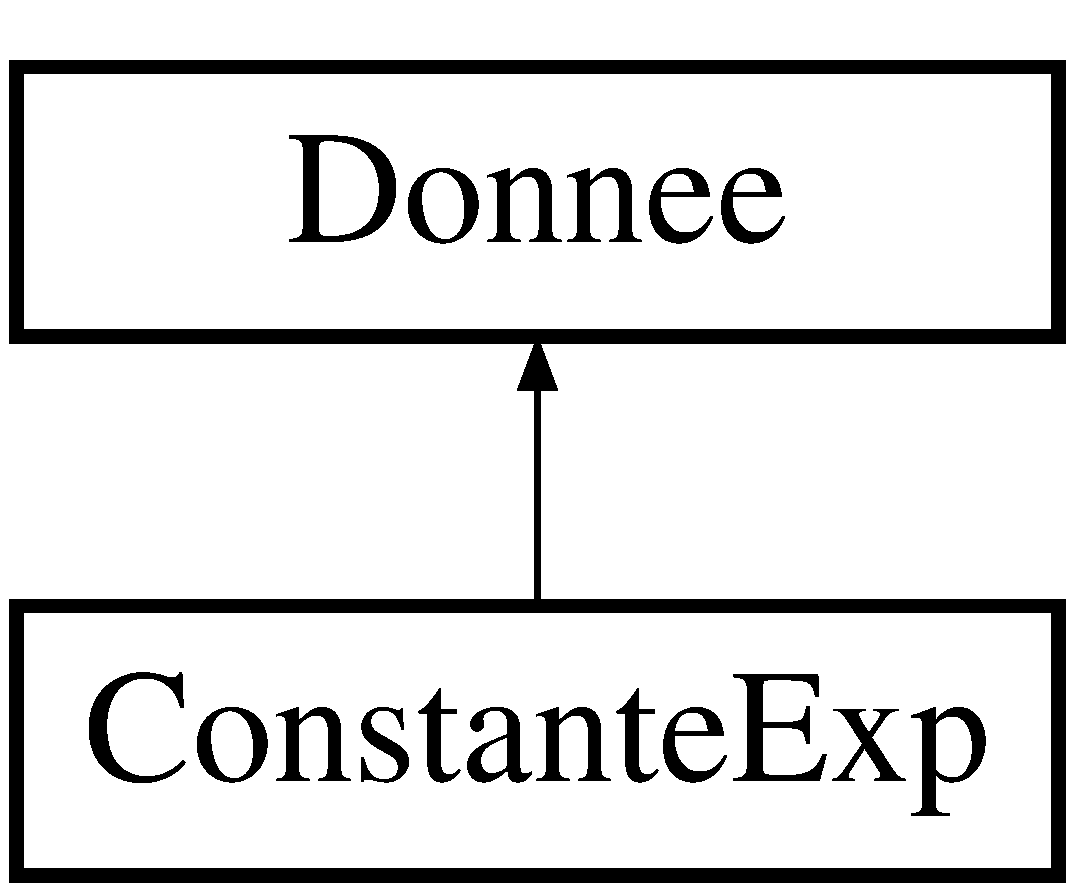
\includegraphics[height=2.000000cm]{class_constante_exp}
\end{center}
\end{figure}
\subsection*{Fonctions membres publiques}
\begin{DoxyCompactItemize}
\item 
\hyperlink{class_constante_exp_a5c67010d0ba1edd4385ca07aeffe1288}{Constante\-Exp} (const Q\-String \&a\-Q\-String)
\begin{DoxyCompactList}\small\item\em Constructeur de \hyperlink{class_constante_exp}{Constante\-Exp} � partir d'une cha�ne de caract�res. \end{DoxyCompactList}\item 
virtual Q\-String \hyperlink{class_constante_exp_acc5010b4a9d9f464a5052700face520d}{to\-Q\-String} () const 
\begin{DoxyCompactList}\small\item\em Renvoie l'expression sous forme de chaine de caract�res. \end{DoxyCompactList}\item 
\hyperlink{class_donnee}{Donnee} $\ast$ \hyperlink{class_constante_exp_a6cc02a6db2905d35750eaca89e99c542}{operator+} (\hyperlink{class_donnee}{Donnee} $\ast$t)
\begin{DoxyCompactList}\small\item\em Operateur +. \end{DoxyCompactList}\item 
\hyperlink{class_donnee}{Donnee} $\ast$ \hyperlink{class_constante_exp_a5f2a2efc405df5feda85a61275f52fd2}{operator/} (\hyperlink{class_donnee}{Donnee} $\ast$t)
\begin{DoxyCompactList}\small\item\em Operateur /. \end{DoxyCompactList}\item 
\hyperlink{class_donnee}{Donnee} $\ast$ \hyperlink{class_constante_exp_a0623fbbea5a736d474905b34a8814104}{operator$\ast$} (\hyperlink{class_donnee}{Donnee} $\ast$t)
\begin{DoxyCompactList}\small\item\em Operateur $\ast$. \end{DoxyCompactList}\item 
\hyperlink{class_donnee}{Donnee} $\ast$ \hyperlink{class_constante_exp_a1b51ec317c0c1ce1ca7cfc7f7103e9ff}{operator-\/} (\hyperlink{class_donnee}{Donnee} $\ast$t)
\begin{DoxyCompactList}\small\item\em Operateur -\/. \end{DoxyCompactList}\item 
virtual \hyperlink{class_donnee}{Donnee} $\ast$ \hyperlink{class_constante_exp_ab3185f222777f91ae1e8aa0cceb630c0}{puissance} (\hyperlink{class_donnee}{Donnee} $\ast$t)
\begin{DoxyCompactList}\small\item\em puissance \end{DoxyCompactList}\item 
virtual \hyperlink{class_donnee}{Donnee} $\ast$ \hyperlink{class_constante_exp_ab2ae3fdd6bd3a5a0a2dd306c7dcf7a9b}{mod} (\hyperlink{class_donnee}{Donnee} $\ast$t)
\begin{DoxyCompactList}\small\item\em mod \end{DoxyCompactList}\item 
Q\-String \hyperlink{class_constante_exp_ae75781451a316c16a6e7fad910121287}{get\-Chaine} () const 
\begin{DoxyCompactList}\small\item\em Accesseur vers l'attribut chaine. \end{DoxyCompactList}\item 
virtual \hyperlink{class_constante_exp}{Constante\-Exp} $\ast$ \hyperlink{class_constante_exp_a12fcc4001e574313ba2e94f3d7ce7847}{sign} ()
\begin{DoxyCompactList}\small\item\em Concat�ne l'op�rateur unaire \hyperlink{class_constante_exp_a12fcc4001e574313ba2e94f3d7ce7847}{sign()} avec l'expression. \end{DoxyCompactList}\item 
virtual \hyperlink{class_donnee}{Donnee} $\ast$ \hyperlink{class_constante_exp_ac19d0914c490b805c430b1132b858e6f}{my\-Sin} (int type\-Angle)
\begin{DoxyCompactList}\small\item\em my\-Sin \end{DoxyCompactList}\item 
virtual \hyperlink{class_donnee}{Donnee} $\ast$ \hyperlink{class_constante_exp_a98fa8756c0e0e3db978882e4702c32db}{my\-Cos} (int type\-Angle)
\begin{DoxyCompactList}\small\item\em my\-Cos \end{DoxyCompactList}\item 
virtual \hyperlink{class_donnee}{Donnee} $\ast$ \hyperlink{class_constante_exp_abdf2718e784d0cee7bb6a0fd1dae7d93}{my\-Tan} (int type\-Angle)
\begin{DoxyCompactList}\small\item\em my\-Tan \end{DoxyCompactList}\item 
virtual \hyperlink{class_donnee}{Donnee} $\ast$ \hyperlink{class_constante_exp_a10b6be5217a36def4768a86acf6b06fd}{my\-Sinh} (int type\-Angle)
\begin{DoxyCompactList}\small\item\em my\-Sinh \end{DoxyCompactList}\item 
virtual \hyperlink{class_donnee}{Donnee} $\ast$ \hyperlink{class_constante_exp_ad5d45910fe58cfd3d4487d5491e51174}{my\-Cosh} (int type\-Angle)
\begin{DoxyCompactList}\small\item\em my\-Cosh \end{DoxyCompactList}\item 
virtual \hyperlink{class_donnee}{Donnee} $\ast$ \hyperlink{class_constante_exp_a8195df51db69a76875b1e93e7d8e9225}{my\-Tanh} (int type\-Angle)
\begin{DoxyCompactList}\small\item\em my\-Tanh \end{DoxyCompactList}\item 
virtual \hyperlink{class_donnee}{Donnee} $\ast$ \hyperlink{class_constante_exp_a1e2b8852cc7bcbdc4ec2f66579946f51}{my\-Ln} ()
\begin{DoxyCompactList}\small\item\em my\-Ln \end{DoxyCompactList}\item 
virtual \hyperlink{class_donnee}{Donnee} $\ast$ \hyperlink{class_constante_exp_a7e503fd204290f196093dbf1ffc23af3}{my\-Log} ()
\begin{DoxyCompactList}\small\item\em my\-Log \end{DoxyCompactList}\item 
virtual \hyperlink{class_donnee}{Donnee} $\ast$ \hyperlink{class_constante_exp_a65b2631d4944be636fa2ebe0088ae581}{my\-Inv} ()
\begin{DoxyCompactList}\small\item\em my\-Inv \end{DoxyCompactList}\item 
virtual \hyperlink{class_donnee}{Donnee} $\ast$ \hyperlink{class_constante_exp_a8a6e86e874617f9f03553a90ace23cfe}{my\-Sqrt} ()
\begin{DoxyCompactList}\small\item\em my\-Sqrt \end{DoxyCompactList}\item 
virtual \hyperlink{class_donnee}{Donnee} $\ast$ \hyperlink{class_constante_exp_acfb9df9f23ee33b8a406b68004cc2238}{my\-Sqr} ()
\begin{DoxyCompactList}\small\item\em my\-Sqr \end{DoxyCompactList}\item 
virtual \hyperlink{class_donnee}{Donnee} $\ast$ \hyperlink{class_constante_exp_a0a4393e85f7024e52bc673475d636264}{my\-Cube} ()
\begin{DoxyCompactList}\small\item\em my\-Cube \end{DoxyCompactList}\item 
virtual \hyperlink{class_donnee}{Donnee} $\ast$ \hyperlink{class_constante_exp_a6f30fd2562442a46c9a1a816fd6d5d7a}{my\-Fact} ()
\begin{DoxyCompactList}\small\item\em my\-Fact \end{DoxyCompactList}\item 
bool \hyperlink{class_constante_exp_af9a973ea5d3d87365c66c93c9bec631f}{is\-Zero} ()
\begin{DoxyCompactList}\small\item\em is\-Zero \end{DoxyCompactList}\item 
bool \hyperlink{class_constante_exp_a604a744c7173c9b9dc94cc7036875e88}{is\-Neg} ()
\begin{DoxyCompactList}\small\item\em is\-Neg \end{DoxyCompactList}\end{DoxyCompactItemize}
\subsection*{Additional Inherited Members}


\subsection{Description détaillée}
Classe regroupant les Constantes Expressions. 

\begin{DoxyAuthor}{Auteur}
Letellier/\-Yassine
\end{DoxyAuthor}
Les objets de cette classe travaillent autour d'une chaine de caract�res. Celle-\/ci d�crit une expression. 

\subsection{Documentation des constructeurs et destructeur}
\hypertarget{class_constante_exp_a5c67010d0ba1edd4385ca07aeffe1288}{\index{Constante\-Exp@{Constante\-Exp}!Constante\-Exp@{Constante\-Exp}}
\index{Constante\-Exp@{Constante\-Exp}!ConstanteExp@{Constante\-Exp}}
\subsubsection[{Constante\-Exp}]{\setlength{\rightskip}{0pt plus 5cm}Constante\-Exp\-::\-Constante\-Exp (
\begin{DoxyParamCaption}
\item[{const Q\-String \&}]{a\-Q\-String}
\end{DoxyParamCaption}
)\hspace{0.3cm}{\ttfamily [inline]}}}\label{class_constante_exp_a5c67010d0ba1edd4385ca07aeffe1288}


Constructeur de \hyperlink{class_constante_exp}{Constante\-Exp} � partir d'une cha�ne de caract�res. 


\begin{DoxyParams}{Paramètres}
{\em a\-Q\-String} & Cha�ne de caract�res � recopier. \\
\hline
\end{DoxyParams}
\begin{DoxyReturn}{Renvoie}
Elle retourne la \hyperlink{class_constante_exp}{Constante\-Exp} construite. 
\end{DoxyReturn}


\subsection{Documentation des fonctions membres}
\hypertarget{class_constante_exp_ae75781451a316c16a6e7fad910121287}{\index{Constante\-Exp@{Constante\-Exp}!get\-Chaine@{get\-Chaine}}
\index{get\-Chaine@{get\-Chaine}!ConstanteExp@{Constante\-Exp}}
\subsubsection[{get\-Chaine}]{\setlength{\rightskip}{0pt plus 5cm}Q\-String Constante\-Exp\-::get\-Chaine (
\begin{DoxyParamCaption}
{}
\end{DoxyParamCaption}
) const\hspace{0.3cm}{\ttfamily [inline]}}}\label{class_constante_exp_ae75781451a316c16a6e7fad910121287}


Accesseur vers l'attribut chaine. 

\begin{DoxyReturn}{Renvoie}
Une Q\-String recopi�e depuis l'attribut chaine. 
\end{DoxyReturn}
\hypertarget{class_constante_exp_a604a744c7173c9b9dc94cc7036875e88}{\index{Constante\-Exp@{Constante\-Exp}!is\-Neg@{is\-Neg}}
\index{is\-Neg@{is\-Neg}!ConstanteExp@{Constante\-Exp}}
\subsubsection[{is\-Neg}]{\setlength{\rightskip}{0pt plus 5cm}bool Constante\-Exp\-::is\-Neg (
\begin{DoxyParamCaption}
{}
\end{DoxyParamCaption}
)\hspace{0.3cm}{\ttfamily [inline]}, {\ttfamily [virtual]}}}\label{class_constante_exp_a604a744c7173c9b9dc94cc7036875e88}


is\-Neg 

Mathode permettant de savoir si la \hyperlink{class_donnee}{Donnee} est inferieure ou egale � 0 \begin{DoxyReturn}{Renvoie}
bool true si la \hyperlink{class_donnee}{Donnee} est inferieur ou egale � 0 
\end{DoxyReturn}


Implémente \hyperlink{class_donnee_a0efb324f0c2e0682b971c3692c46e7c3}{Donnee}.

\hypertarget{class_constante_exp_af9a973ea5d3d87365c66c93c9bec631f}{\index{Constante\-Exp@{Constante\-Exp}!is\-Zero@{is\-Zero}}
\index{is\-Zero@{is\-Zero}!ConstanteExp@{Constante\-Exp}}
\subsubsection[{is\-Zero}]{\setlength{\rightskip}{0pt plus 5cm}bool Constante\-Exp\-::is\-Zero (
\begin{DoxyParamCaption}
{}
\end{DoxyParamCaption}
)\hspace{0.3cm}{\ttfamily [inline]}, {\ttfamily [virtual]}}}\label{class_constante_exp_af9a973ea5d3d87365c66c93c9bec631f}


is\-Zero 

Mathode permettant de savoir si la \hyperlink{class_donnee}{Donnee} est egale � 0 \begin{DoxyReturn}{Renvoie}
bool true si la \hyperlink{class_donnee}{Donnee} est egale � 0 
\end{DoxyReturn}


Implémente \hyperlink{class_donnee_aad251e4148c791719d7d7bff18680611}{Donnee}.

\hypertarget{class_constante_exp_ab2ae3fdd6bd3a5a0a2dd306c7dcf7a9b}{\index{Constante\-Exp@{Constante\-Exp}!mod@{mod}}
\index{mod@{mod}!ConstanteExp@{Constante\-Exp}}
\subsubsection[{mod}]{\setlength{\rightskip}{0pt plus 5cm}{\bf Donnee} $\ast$ Constante\-Exp\-::mod (
\begin{DoxyParamCaption}
\item[{{\bf Donnee} $\ast$}]{t}
\end{DoxyParamCaption}
)\hspace{0.3cm}{\ttfamily [virtual]}}}\label{class_constante_exp_ab2ae3fdd6bd3a5a0a2dd306c7dcf7a9b}


mod 

Implementation de l'op�rateur binaire modulo (methode virtuelle dans la classe mere) 
\begin{DoxyParams}{Paramètres}
{\em Donnee$\ast$,\-:} & Pointeur sur une donnee \\
\hline
\end{DoxyParams}
\begin{DoxyReturn}{Renvoie}
Pointeur sur donnee, resultat de l'operation 
\end{DoxyReturn}


Implémente \hyperlink{class_donnee_a52ce1aa17ce2c613e98428f82e3f85b8}{Donnee}.

\hypertarget{class_constante_exp_a98fa8756c0e0e3db978882e4702c32db}{\index{Constante\-Exp@{Constante\-Exp}!my\-Cos@{my\-Cos}}
\index{my\-Cos@{my\-Cos}!ConstanteExp@{Constante\-Exp}}
\subsubsection[{my\-Cos}]{\setlength{\rightskip}{0pt plus 5cm}{\bf Donnee} $\ast$ Constante\-Exp\-::my\-Cos (
\begin{DoxyParamCaption}
\item[{int}]{type\-Angle}
\end{DoxyParamCaption}
)\hspace{0.3cm}{\ttfamily [virtual]}}}\label{class_constante_exp_a98fa8756c0e0e3db978882e4702c32db}


my\-Cos 

Implementation de l'op�rateur unaire cosinus (methode virtuelle dans la classe mere) 
\begin{DoxyParams}{Paramètres}
{\em type\-Angle} & \-: entier, 0 si utilisation des degres, 1 si utilisation des radians \\
\hline
\end{DoxyParams}
\begin{DoxyReturn}{Renvoie}
Pointeur sur donnee, resultat de l'operation 
\end{DoxyReturn}


Implémente \hyperlink{class_donnee_abd9a62bd6b7d189f50db350823e895c3}{Donnee}.

\hypertarget{class_constante_exp_ad5d45910fe58cfd3d4487d5491e51174}{\index{Constante\-Exp@{Constante\-Exp}!my\-Cosh@{my\-Cosh}}
\index{my\-Cosh@{my\-Cosh}!ConstanteExp@{Constante\-Exp}}
\subsubsection[{my\-Cosh}]{\setlength{\rightskip}{0pt plus 5cm}{\bf Donnee} $\ast$ Constante\-Exp\-::my\-Cosh (
\begin{DoxyParamCaption}
\item[{int}]{type\-Angle}
\end{DoxyParamCaption}
)\hspace{0.3cm}{\ttfamily [virtual]}}}\label{class_constante_exp_ad5d45910fe58cfd3d4487d5491e51174}


my\-Cosh 

Implementation de l'op�rateur unaire cosinush (methode virtuelle dans la classe mere) 
\begin{DoxyParams}{Paramètres}
{\em type\-Angle} & \-: entier, 0 si utilisation des degres, 1 si utilisation des radians \\
\hline
\end{DoxyParams}
\begin{DoxyReturn}{Renvoie}
Pointeur sur donnee, resultat de l'operation 
\end{DoxyReturn}


Implémente \hyperlink{class_donnee_afe9b3532677d394b4b596021b74b6d17}{Donnee}.

\hypertarget{class_constante_exp_a0a4393e85f7024e52bc673475d636264}{\index{Constante\-Exp@{Constante\-Exp}!my\-Cube@{my\-Cube}}
\index{my\-Cube@{my\-Cube}!ConstanteExp@{Constante\-Exp}}
\subsubsection[{my\-Cube}]{\setlength{\rightskip}{0pt plus 5cm}{\bf Donnee} $\ast$ Constante\-Exp\-::my\-Cube (
\begin{DoxyParamCaption}
{}
\end{DoxyParamCaption}
)\hspace{0.3cm}{\ttfamily [virtual]}}}\label{class_constante_exp_a0a4393e85f7024e52bc673475d636264}


my\-Cube 

Implementation de l'op�rateur unaire Cube (methode virtuelle dans la classe mere) \begin{DoxyReturn}{Renvoie}
Pointeur sur donnee, resultat de l'operation 
\end{DoxyReturn}


Implémente \hyperlink{class_donnee_a875c21efdd22695c7999cfeb52ce4b2a}{Donnee}.

\hypertarget{class_constante_exp_a6f30fd2562442a46c9a1a816fd6d5d7a}{\index{Constante\-Exp@{Constante\-Exp}!my\-Fact@{my\-Fact}}
\index{my\-Fact@{my\-Fact}!ConstanteExp@{Constante\-Exp}}
\subsubsection[{my\-Fact}]{\setlength{\rightskip}{0pt plus 5cm}{\bf Donnee} $\ast$ Constante\-Exp\-::my\-Fact (
\begin{DoxyParamCaption}
{}
\end{DoxyParamCaption}
)\hspace{0.3cm}{\ttfamily [virtual]}}}\label{class_constante_exp_a6f30fd2562442a46c9a1a816fd6d5d7a}


my\-Fact 

Implementation de l'op�rateur unaire fact (methode virtuelle dans la classe mere) \begin{DoxyReturn}{Renvoie}
Pointeur sur donnee, resultat de l'operation 
\end{DoxyReturn}


Implémente \hyperlink{class_donnee_a79a2a3f835e09d0ed1888800c595a715}{Donnee}.

\hypertarget{class_constante_exp_a65b2631d4944be636fa2ebe0088ae581}{\index{Constante\-Exp@{Constante\-Exp}!my\-Inv@{my\-Inv}}
\index{my\-Inv@{my\-Inv}!ConstanteExp@{Constante\-Exp}}
\subsubsection[{my\-Inv}]{\setlength{\rightskip}{0pt plus 5cm}{\bf Donnee} $\ast$ Constante\-Exp\-::my\-Inv (
\begin{DoxyParamCaption}
{}
\end{DoxyParamCaption}
)\hspace{0.3cm}{\ttfamily [virtual]}}}\label{class_constante_exp_a65b2631d4944be636fa2ebe0088ae581}


my\-Inv 

Implementation de l'op�rateur unaire inv (methode virtuelle dans la classe mere) \begin{DoxyReturn}{Renvoie}
Pointeur sur donnee, resultat de l'operation 
\end{DoxyReturn}


Implémente \hyperlink{class_donnee_ad84c463eb43d4b98bed081045160fea1}{Donnee}.

\hypertarget{class_constante_exp_a1e2b8852cc7bcbdc4ec2f66579946f51}{\index{Constante\-Exp@{Constante\-Exp}!my\-Ln@{my\-Ln}}
\index{my\-Ln@{my\-Ln}!ConstanteExp@{Constante\-Exp}}
\subsubsection[{my\-Ln}]{\setlength{\rightskip}{0pt plus 5cm}{\bf Donnee} $\ast$ Constante\-Exp\-::my\-Ln (
\begin{DoxyParamCaption}
{}
\end{DoxyParamCaption}
)\hspace{0.3cm}{\ttfamily [virtual]}}}\label{class_constante_exp_a1e2b8852cc7bcbdc4ec2f66579946f51}


my\-Ln 

Implementation de l'op�rateur unaire ln (methode virtuelle dans la classe mere) \begin{DoxyReturn}{Renvoie}
Pointeur sur donnee, resultat de l'operation 
\end{DoxyReturn}


Implémente \hyperlink{class_donnee_ac24ba41baf90eb99bcf91145c541780a}{Donnee}.

\hypertarget{class_constante_exp_a7e503fd204290f196093dbf1ffc23af3}{\index{Constante\-Exp@{Constante\-Exp}!my\-Log@{my\-Log}}
\index{my\-Log@{my\-Log}!ConstanteExp@{Constante\-Exp}}
\subsubsection[{my\-Log}]{\setlength{\rightskip}{0pt plus 5cm}{\bf Donnee} $\ast$ Constante\-Exp\-::my\-Log (
\begin{DoxyParamCaption}
{}
\end{DoxyParamCaption}
)\hspace{0.3cm}{\ttfamily [virtual]}}}\label{class_constante_exp_a7e503fd204290f196093dbf1ffc23af3}


my\-Log 

Implementation de l'op�rateur unaire log (methode virtuelle dans la classe mere) \begin{DoxyReturn}{Renvoie}
Pointeur sur donnee, resultat de l'operation 
\end{DoxyReturn}


Implémente \hyperlink{class_donnee_a7ac3f554be1fc579b02d9c877185cf50}{Donnee}.

\hypertarget{class_constante_exp_ac19d0914c490b805c430b1132b858e6f}{\index{Constante\-Exp@{Constante\-Exp}!my\-Sin@{my\-Sin}}
\index{my\-Sin@{my\-Sin}!ConstanteExp@{Constante\-Exp}}
\subsubsection[{my\-Sin}]{\setlength{\rightskip}{0pt plus 5cm}{\bf Donnee} $\ast$ Constante\-Exp\-::my\-Sin (
\begin{DoxyParamCaption}
\item[{int}]{type\-Angle}
\end{DoxyParamCaption}
)\hspace{0.3cm}{\ttfamily [virtual]}}}\label{class_constante_exp_ac19d0914c490b805c430b1132b858e6f}


my\-Sin 

Implementation de l'op�rateur unaire sinus (methode virtuelle dans la classe mere) 
\begin{DoxyParams}{Paramètres}
{\em type\-Angle} & \-: entier, 0 si utilisation des degres, 1 si utilisation des radians \\
\hline
\end{DoxyParams}
\begin{DoxyReturn}{Renvoie}
Pointeur sur donnee, resultat de l'operation 
\end{DoxyReturn}


Implémente \hyperlink{class_donnee_a86f71d87c3a69dc6dcede4b411d94043}{Donnee}.

\hypertarget{class_constante_exp_a10b6be5217a36def4768a86acf6b06fd}{\index{Constante\-Exp@{Constante\-Exp}!my\-Sinh@{my\-Sinh}}
\index{my\-Sinh@{my\-Sinh}!ConstanteExp@{Constante\-Exp}}
\subsubsection[{my\-Sinh}]{\setlength{\rightskip}{0pt plus 5cm}{\bf Donnee} $\ast$ Constante\-Exp\-::my\-Sinh (
\begin{DoxyParamCaption}
\item[{int}]{type\-Angle}
\end{DoxyParamCaption}
)\hspace{0.3cm}{\ttfamily [virtual]}}}\label{class_constante_exp_a10b6be5217a36def4768a86acf6b06fd}


my\-Sinh 

Implementation de l'op�rateur unaire sinush (methode virtuelle dans la classe mere) 
\begin{DoxyParams}{Paramètres}
{\em type\-Angle} & \-: entier, 0 si utilisation des degres, 1 si utilisation des radians \\
\hline
\end{DoxyParams}
\begin{DoxyReturn}{Renvoie}
Pointeur sur donnee, resultat de l'operation 
\end{DoxyReturn}


Implémente \hyperlink{class_donnee_af3c408a3fda8f24ee70f34fd8688fe63}{Donnee}.

\hypertarget{class_constante_exp_acfb9df9f23ee33b8a406b68004cc2238}{\index{Constante\-Exp@{Constante\-Exp}!my\-Sqr@{my\-Sqr}}
\index{my\-Sqr@{my\-Sqr}!ConstanteExp@{Constante\-Exp}}
\subsubsection[{my\-Sqr}]{\setlength{\rightskip}{0pt plus 5cm}{\bf Donnee} $\ast$ Constante\-Exp\-::my\-Sqr (
\begin{DoxyParamCaption}
{}
\end{DoxyParamCaption}
)\hspace{0.3cm}{\ttfamily [virtual]}}}\label{class_constante_exp_acfb9df9f23ee33b8a406b68004cc2238}


my\-Sqr 

Implementation de l'op�rateur unaire sqr (methode virtuelle dans la classe mere) \begin{DoxyReturn}{Renvoie}
Pointeur sur donnee, resultat de l'operation 
\end{DoxyReturn}


Implémente \hyperlink{class_donnee_a708281bf8ddb3f6c33a100b3db925901}{Donnee}.

\hypertarget{class_constante_exp_a8a6e86e874617f9f03553a90ace23cfe}{\index{Constante\-Exp@{Constante\-Exp}!my\-Sqrt@{my\-Sqrt}}
\index{my\-Sqrt@{my\-Sqrt}!ConstanteExp@{Constante\-Exp}}
\subsubsection[{my\-Sqrt}]{\setlength{\rightskip}{0pt plus 5cm}{\bf Donnee} $\ast$ Constante\-Exp\-::my\-Sqrt (
\begin{DoxyParamCaption}
{}
\end{DoxyParamCaption}
)\hspace{0.3cm}{\ttfamily [virtual]}}}\label{class_constante_exp_a8a6e86e874617f9f03553a90ace23cfe}


my\-Sqrt 

Implementation de l'op�rateur unaire sqrt (methode virtuelle dans la classe mere) \begin{DoxyReturn}{Renvoie}
Pointeur sur donnee, resultat de l'operation 
\end{DoxyReturn}


Implémente \hyperlink{class_donnee_a07484cd79bc071fbfc48ace5bcd94e8f}{Donnee}.

\hypertarget{class_constante_exp_abdf2718e784d0cee7bb6a0fd1dae7d93}{\index{Constante\-Exp@{Constante\-Exp}!my\-Tan@{my\-Tan}}
\index{my\-Tan@{my\-Tan}!ConstanteExp@{Constante\-Exp}}
\subsubsection[{my\-Tan}]{\setlength{\rightskip}{0pt plus 5cm}{\bf Donnee} $\ast$ Constante\-Exp\-::my\-Tan (
\begin{DoxyParamCaption}
\item[{int}]{type\-Angle}
\end{DoxyParamCaption}
)\hspace{0.3cm}{\ttfamily [virtual]}}}\label{class_constante_exp_abdf2718e784d0cee7bb6a0fd1dae7d93}


my\-Tan 

Implementation de l'op�rateur unaire tangente (methode virtuelle dans la classe mere) 
\begin{DoxyParams}{Paramètres}
{\em type\-Angle} & \-: entier, 0 si utilisation des degres, 1 si utilisation des radians \\
\hline
\end{DoxyParams}
\begin{DoxyReturn}{Renvoie}
Pointeur sur donnee, resultat de l'operation 
\end{DoxyReturn}


Implémente \hyperlink{class_donnee_ad3b4b9d20c0693915d9c17b528bed4d8}{Donnee}.

\hypertarget{class_constante_exp_a8195df51db69a76875b1e93e7d8e9225}{\index{Constante\-Exp@{Constante\-Exp}!my\-Tanh@{my\-Tanh}}
\index{my\-Tanh@{my\-Tanh}!ConstanteExp@{Constante\-Exp}}
\subsubsection[{my\-Tanh}]{\setlength{\rightskip}{0pt plus 5cm}{\bf Donnee} $\ast$ Constante\-Exp\-::my\-Tanh (
\begin{DoxyParamCaption}
\item[{int}]{type\-Angle}
\end{DoxyParamCaption}
)\hspace{0.3cm}{\ttfamily [virtual]}}}\label{class_constante_exp_a8195df51db69a76875b1e93e7d8e9225}


my\-Tanh 

Implementation de l'op�rateur unaire tangenteh (methode virtuelle dans la classe mere) 
\begin{DoxyParams}{Paramètres}
{\em type\-Angle} & \-: entier, 0 si utilisation des degres, 1 si utilisation des radians \\
\hline
\end{DoxyParams}
\begin{DoxyReturn}{Renvoie}
Pointeur sur donnee, resultat de l'operation 
\end{DoxyReturn}


Implémente \hyperlink{class_donnee_a20a90ca79d91dc75ea01cc3842b0e6dd}{Donnee}.

\hypertarget{class_constante_exp_a0623fbbea5a736d474905b34a8814104}{\index{Constante\-Exp@{Constante\-Exp}!operator$\ast$@{operator$\ast$}}
\index{operator$\ast$@{operator$\ast$}!ConstanteExp@{Constante\-Exp}}
\subsubsection[{operator$\ast$}]{\setlength{\rightskip}{0pt plus 5cm}{\bf Donnee} $\ast$ Constante\-Exp\-::operator$\ast$ (
\begin{DoxyParamCaption}
\item[{{\bf Donnee} $\ast$}]{t}
\end{DoxyParamCaption}
)\hspace{0.3cm}{\ttfamily [virtual]}}}\label{class_constante_exp_a0623fbbea5a736d474905b34a8814104}


Operateur $\ast$. 

Implementation de l'op�rateur binaire $\ast$ (methode virtuelle dans la classe mere) 
\begin{DoxyParams}{Paramètres}
{\em t} & \-: Pointeur sur un type \\
\hline
\end{DoxyParams}
\begin{DoxyReturn}{Renvoie}
Pointeur sur type, resultat de l'operation 
\end{DoxyReturn}


Implémente \hyperlink{class_donnee_ae655c41f021de91a35d652a8519d4eb2}{Donnee}.

\hypertarget{class_constante_exp_a6cc02a6db2905d35750eaca89e99c542}{\index{Constante\-Exp@{Constante\-Exp}!operator+@{operator+}}
\index{operator+@{operator+}!ConstanteExp@{Constante\-Exp}}
\subsubsection[{operator+}]{\setlength{\rightskip}{0pt plus 5cm}{\bf Donnee} $\ast$ Constante\-Exp\-::operator+ (
\begin{DoxyParamCaption}
\item[{{\bf Donnee} $\ast$}]{t}
\end{DoxyParamCaption}
)\hspace{0.3cm}{\ttfamily [virtual]}}}\label{class_constante_exp_a6cc02a6db2905d35750eaca89e99c542}


Operateur +. 

Implementation de l'op�rateur binaire + (methode virtuelle dans la classe mere) 
\begin{DoxyParams}{Paramètres}
{\em t} & \-: Pointeur sur un type \\
\hline
\end{DoxyParams}
\begin{DoxyReturn}{Renvoie}
Pointeur sur type, resultat de l'operation 
\end{DoxyReturn}


Implémente \hyperlink{class_donnee_acda2976724adeef2233e7077953c1a9a}{Donnee}.

\hypertarget{class_constante_exp_a1b51ec317c0c1ce1ca7cfc7f7103e9ff}{\index{Constante\-Exp@{Constante\-Exp}!operator-\/@{operator-\/}}
\index{operator-\/@{operator-\/}!ConstanteExp@{Constante\-Exp}}
\subsubsection[{operator-\/}]{\setlength{\rightskip}{0pt plus 5cm}{\bf Donnee} $\ast$ Constante\-Exp\-::operator-\/ (
\begin{DoxyParamCaption}
\item[{{\bf Donnee} $\ast$}]{t}
\end{DoxyParamCaption}
)\hspace{0.3cm}{\ttfamily [virtual]}}}\label{class_constante_exp_a1b51ec317c0c1ce1ca7cfc7f7103e9ff}


Operateur -\/. 

Implementation de l'op�rateur binaire -\/ (methode virtuelle dans la classe mere) 
\begin{DoxyParams}{Paramètres}
{\em t} & \-: Pointeur sur un type \\
\hline
\end{DoxyParams}
\begin{DoxyReturn}{Renvoie}
Pointeur sur type, resultat de l'operation 
\end{DoxyReturn}


Implémente \hyperlink{class_donnee_a053ea4f3f00b6e0a73b4ea453adca1be}{Donnee}.

\hypertarget{class_constante_exp_a5f2a2efc405df5feda85a61275f52fd2}{\index{Constante\-Exp@{Constante\-Exp}!operator/@{operator/}}
\index{operator/@{operator/}!ConstanteExp@{Constante\-Exp}}
\subsubsection[{operator/}]{\setlength{\rightskip}{0pt plus 5cm}{\bf Donnee} $\ast$ Constante\-Exp\-::operator/ (
\begin{DoxyParamCaption}
\item[{{\bf Donnee} $\ast$}]{t}
\end{DoxyParamCaption}
)\hspace{0.3cm}{\ttfamily [virtual]}}}\label{class_constante_exp_a5f2a2efc405df5feda85a61275f52fd2}


Operateur /. 

Implementation de l'op�rateur binaire / (methode virtuelle dans la classe mere) 
\begin{DoxyParams}{Paramètres}
{\em t} & \-: Pointeur sur un type \\
\hline
\end{DoxyParams}
\begin{DoxyReturn}{Renvoie}
Pointeur sur type, resultat de l'operation 
\end{DoxyReturn}


Implémente \hyperlink{class_donnee_abc63ffa0d62612446435ff1eca34344b}{Donnee}.

\hypertarget{class_constante_exp_ab3185f222777f91ae1e8aa0cceb630c0}{\index{Constante\-Exp@{Constante\-Exp}!puissance@{puissance}}
\index{puissance@{puissance}!ConstanteExp@{Constante\-Exp}}
\subsubsection[{puissance}]{\setlength{\rightskip}{0pt plus 5cm}{\bf Donnee} $\ast$ Constante\-Exp\-::puissance (
\begin{DoxyParamCaption}
\item[{{\bf Donnee} $\ast$}]{t}
\end{DoxyParamCaption}
)\hspace{0.3cm}{\ttfamily [virtual]}}}\label{class_constante_exp_ab3185f222777f91ae1e8aa0cceb630c0}


puissance 

Implementation de l'op�rateur binaire puissance (methode virtuelle dans la classe mere) 
\begin{DoxyParams}{Paramètres}
{\em Donnee$\ast$,\-:} & Pointeur sur une donnee \\
\hline
\end{DoxyParams}
\begin{DoxyReturn}{Renvoie}
Pointeur sur donnee, resultat de l'operation 
\end{DoxyReturn}


Implémente \hyperlink{class_donnee_af25f76885c91b1a497023c9dd2231990}{Donnee}.

\hypertarget{class_constante_exp_a12fcc4001e574313ba2e94f3d7ce7847}{\index{Constante\-Exp@{Constante\-Exp}!sign@{sign}}
\index{sign@{sign}!ConstanteExp@{Constante\-Exp}}
\subsubsection[{sign}]{\setlength{\rightskip}{0pt plus 5cm}{\bf Constante\-Exp} $\ast$ Constante\-Exp\-::sign (
\begin{DoxyParamCaption}
{}
\end{DoxyParamCaption}
)\hspace{0.3cm}{\ttfamily [virtual]}}}\label{class_constante_exp_a12fcc4001e574313ba2e94f3d7ce7847}


Concat�ne l'op�rateur unaire \hyperlink{class_constante_exp_a12fcc4001e574313ba2e94f3d7ce7847}{sign()} avec l'expression. 

\begin{DoxyReturn}{Renvoie}
Elle retourne le nouvel objet. 
\end{DoxyReturn}


Implémente \hyperlink{class_donnee_a3a2d30e5c70d0a6d74a4282dc31841a9}{Donnee}.

\hypertarget{class_constante_exp_acc5010b4a9d9f464a5052700face520d}{\index{Constante\-Exp@{Constante\-Exp}!to\-Q\-String@{to\-Q\-String}}
\index{to\-Q\-String@{to\-Q\-String}!ConstanteExp@{Constante\-Exp}}
\subsubsection[{to\-Q\-String}]{\setlength{\rightskip}{0pt plus 5cm}virtual Q\-String Constante\-Exp\-::to\-Q\-String (
\begin{DoxyParamCaption}
{}
\end{DoxyParamCaption}
) const\hspace{0.3cm}{\ttfamily [inline]}, {\ttfamily [virtual]}}}\label{class_constante_exp_acc5010b4a9d9f464a5052700face520d}


Renvoie l'expression sous forme de chaine de caract�res. 

\begin{DoxyReturn}{Renvoie}
La chaine de caract�res contenant l'expression est retourn�e. 
\end{DoxyReturn}


Implémente \hyperlink{class_donnee_ad96590e462f8db33aefca28ba8e31e52}{Donnee}.



La documentation de cette classe a été générée à partir des fichiers suivants \-:\begin{DoxyCompactItemize}
\item 
\hyperlink{constanteexp_8h}{constanteexp.\-h}\item 
constanteexp.\-cpp\end{DoxyCompactItemize}

\hypertarget{class_donnee}{\section{Donnee Class Reference}
\label{class_donnee}\index{Donnee@{Donnee}}
}
Inheritance diagram for Donnee\-:\begin{figure}[H]
\begin{center}
\leavevmode
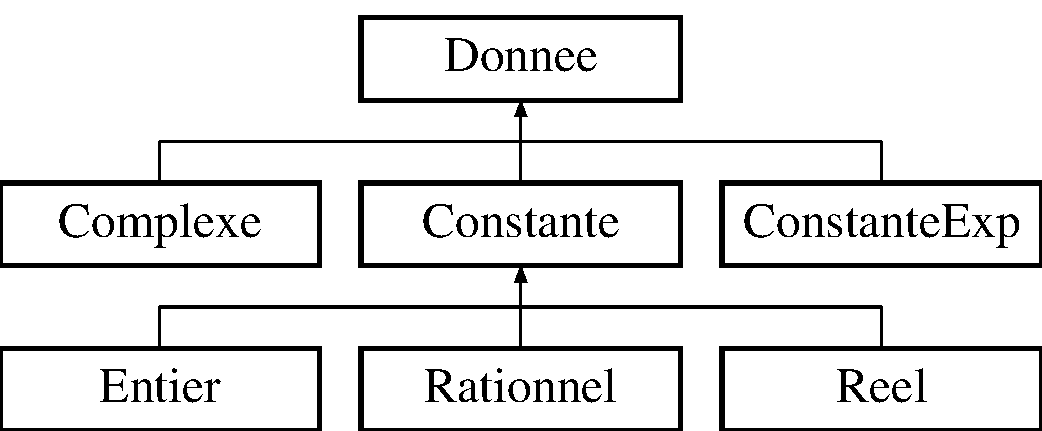
\includegraphics[height=3.000000cm]{class_donnee}
\end{center}
\end{figure}
\subsection*{Public Member Functions}
\begin{DoxyCompactItemize}
\item 
\hypertarget{class_donnee_a6d12ca05456653bb849513dce31ba1a7}{\hyperlink{class_donnee_a6d12ca05456653bb849513dce31ba1a7}{Donnee} ()}\label{class_donnee_a6d12ca05456653bb849513dce31ba1a7}

\begin{DoxyCompactList}\small\item\em Constructeur sans arguments de \hyperlink{class_donnee}{Donnee}. \end{DoxyCompactList}\item 
virtual Q\-String \hyperlink{class_donnee_ad96590e462f8db33aefca28ba8e31e52}{to\-Q\-String} () const =0
\begin{DoxyCompactList}\small\item\em M�thode permettant d'obtenir l'objet sous la forme d'une Q\-String. \end{DoxyCompactList}\item 
virtual \hyperlink{class_donnee}{Donnee} $\ast$ \hyperlink{class_donnee_acda2976724adeef2233e7077953c1a9a}{operator+} (\hyperlink{class_donnee}{Donnee} $\ast$t)=0
\begin{DoxyCompactList}\small\item\em Operateur +. \end{DoxyCompactList}\item 
virtual \hyperlink{class_donnee}{Donnee} $\ast$ \hyperlink{class_donnee_abc63ffa0d62612446435ff1eca34344b}{operator/} (\hyperlink{class_donnee}{Donnee} $\ast$t)=0
\begin{DoxyCompactList}\small\item\em Operateur /. \end{DoxyCompactList}\item 
virtual \hyperlink{class_donnee}{Donnee} $\ast$ \hyperlink{class_donnee_ae655c41f021de91a35d652a8519d4eb2}{operator$\ast$} (\hyperlink{class_donnee}{Donnee} $\ast$t)=0
\begin{DoxyCompactList}\small\item\em Operateur $\ast$. \end{DoxyCompactList}\item 
virtual \hyperlink{class_donnee}{Donnee} $\ast$ \hyperlink{class_donnee_a053ea4f3f00b6e0a73b4ea453adca1be}{operator-\/} (\hyperlink{class_donnee}{Donnee} $\ast$t)=0
\begin{DoxyCompactList}\small\item\em Operateur -\/. \end{DoxyCompactList}\item 
virtual \hyperlink{class_donnee}{Donnee} $\ast$ \hyperlink{class_donnee_af25f76885c91b1a497023c9dd2231990}{puissance} (\hyperlink{class_donnee}{Donnee} $\ast$t)=0
\begin{DoxyCompactList}\small\item\em puissance \end{DoxyCompactList}\item 
virtual \hyperlink{class_donnee}{Donnee} $\ast$ \hyperlink{class_donnee_a52ce1aa17ce2c613e98428f82e3f85b8}{mod} (\hyperlink{class_donnee}{Donnee} $\ast$t)=0
\begin{DoxyCompactList}\small\item\em mod \end{DoxyCompactList}\item 
virtual \hyperlink{class_donnee}{Donnee} $\ast$ \hyperlink{class_donnee_a3a2d30e5c70d0a6d74a4282dc31841a9}{sign} ()=0
\begin{DoxyCompactList}\small\item\em Retourne une \hyperlink{class_donnee}{Donnee} ayant les memes valeurs mais avec le signe invers� \end{DoxyCompactList}\item 
virtual \hyperlink{class_donnee}{Donnee} $\ast$ \hyperlink{class_donnee_a86f71d87c3a69dc6dcede4b411d94043}{my\-Sin} (int type\-Angle)=0
\begin{DoxyCompactList}\small\item\em my\-Sin \end{DoxyCompactList}\item 
virtual \hyperlink{class_donnee}{Donnee} $\ast$ \hyperlink{class_donnee_abd9a62bd6b7d189f50db350823e895c3}{my\-Cos} (int type\-Angle)=0
\begin{DoxyCompactList}\small\item\em my\-Cos \end{DoxyCompactList}\item 
virtual \hyperlink{class_donnee}{Donnee} $\ast$ \hyperlink{class_donnee_ad3b4b9d20c0693915d9c17b528bed4d8}{my\-Tan} (int type\-Angle)=0
\begin{DoxyCompactList}\small\item\em my\-Tan \end{DoxyCompactList}\item 
virtual \hyperlink{class_donnee}{Donnee} $\ast$ \hyperlink{class_donnee_af3c408a3fda8f24ee70f34fd8688fe63}{my\-Sinh} (int type\-Angle)=0
\begin{DoxyCompactList}\small\item\em my\-Sinh \end{DoxyCompactList}\item 
virtual \hyperlink{class_donnee}{Donnee} $\ast$ \hyperlink{class_donnee_afe9b3532677d394b4b596021b74b6d17}{my\-Cosh} (int type\-Angle)=0
\begin{DoxyCompactList}\small\item\em my\-Cosh \end{DoxyCompactList}\item 
virtual \hyperlink{class_donnee}{Donnee} $\ast$ \hyperlink{class_donnee_a20a90ca79d91dc75ea01cc3842b0e6dd}{my\-Tanh} (int type\-Angle)=0
\begin{DoxyCompactList}\small\item\em my\-Tanh \end{DoxyCompactList}\item 
virtual \hyperlink{class_donnee}{Donnee} $\ast$ \hyperlink{class_donnee_ac24ba41baf90eb99bcf91145c541780a}{my\-Ln} ()=0
\begin{DoxyCompactList}\small\item\em my\-Ln \end{DoxyCompactList}\item 
virtual \hyperlink{class_donnee}{Donnee} $\ast$ \hyperlink{class_donnee_a7ac3f554be1fc579b02d9c877185cf50}{my\-Log} ()=0
\begin{DoxyCompactList}\small\item\em my\-Log \end{DoxyCompactList}\item 
virtual \hyperlink{class_donnee}{Donnee} $\ast$ \hyperlink{class_donnee_ad84c463eb43d4b98bed081045160fea1}{my\-Inv} ()=0
\begin{DoxyCompactList}\small\item\em my\-Inv \end{DoxyCompactList}\item 
virtual \hyperlink{class_donnee}{Donnee} $\ast$ \hyperlink{class_donnee_a07484cd79bc071fbfc48ace5bcd94e8f}{my\-Sqrt} ()=0
\begin{DoxyCompactList}\small\item\em my\-Sqrt \end{DoxyCompactList}\item 
virtual \hyperlink{class_donnee}{Donnee} $\ast$ \hyperlink{class_donnee_a708281bf8ddb3f6c33a100b3db925901}{my\-Sqr} ()=0
\begin{DoxyCompactList}\small\item\em my\-Sqr \end{DoxyCompactList}\item 
virtual \hyperlink{class_donnee}{Donnee} $\ast$ \hyperlink{class_donnee_a875c21efdd22695c7999cfeb52ce4b2a}{my\-Cube} ()=0
\begin{DoxyCompactList}\small\item\em my\-Cube \end{DoxyCompactList}\item 
virtual \hyperlink{class_donnee}{Donnee} $\ast$ \hyperlink{class_donnee_a79a2a3f835e09d0ed1888800c595a715}{my\-Fact} ()=0
\begin{DoxyCompactList}\small\item\em my\-Fact \end{DoxyCompactList}\item 
virtual bool \hyperlink{class_donnee_aad251e4148c791719d7d7bff18680611}{is\-Zero} ()=0
\begin{DoxyCompactList}\small\item\em is\-Zero \end{DoxyCompactList}\item 
virtual bool \hyperlink{class_donnee_a0efb324f0c2e0682b971c3692c46e7c3}{is\-Neg} ()=0
\begin{DoxyCompactList}\small\item\em is\-Neg \end{DoxyCompactList}\end{DoxyCompactItemize}
\subsection*{Static Public Member Functions}
\begin{DoxyCompactItemize}
\item 
static bool \hyperlink{class_donnee_ab195ba9c738ca7a68e46619c05efc25d}{is\-Entier} (const Q\-String \&s)
\begin{DoxyCompactList}\small\item\em is\-Entier Methode statique permettant de determiner le type avec Qregexp \end{DoxyCompactList}\item 
static bool \hyperlink{class_donnee_a3bf8894c20219f055032e5811606e248}{is\-Reel} (const Q\-String \&s)
\begin{DoxyCompactList}\small\item\em is\-Reel Methode statique permettant de determiner le type \end{DoxyCompactList}\item 
static bool \hyperlink{class_donnee_af485090a75b51f1784d60e55a1eefd1a}{is\-Rationnel} (const Q\-String \&s)
\begin{DoxyCompactList}\small\item\em is\-Rationnel Methode statique permettant de determiner le type (Utiisation de regexp) \end{DoxyCompactList}\item 
static bool \hyperlink{class_donnee_a44a63601c9d70c1a99d9c784df740fbb}{is\-Expression} (const Q\-String \&s)
\begin{DoxyCompactList}\small\item\em is\-Expression Methode statique permettant de determiner le type \end{DoxyCompactList}\item 
static bool \hyperlink{class_donnee_aef26bb261eb570e0ba2094f24ceb5eee}{is\-Complexe} (const Q\-String \&s)
\begin{DoxyCompactList}\small\item\em is\-Complexe Methode statique permettant de determiner le type \end{DoxyCompactList}\end{DoxyCompactItemize}


\subsection{Member Function Documentation}
\hypertarget{class_donnee_aef26bb261eb570e0ba2094f24ceb5eee}{\index{Donnee@{Donnee}!is\-Complexe@{is\-Complexe}}
\index{is\-Complexe@{is\-Complexe}!Donnee@{Donnee}}
\subsubsection[{is\-Complexe}]{\setlength{\rightskip}{0pt plus 5cm}static bool Donnee\-::is\-Complexe (
\begin{DoxyParamCaption}
\item[{const Q\-String \&}]{s}
\end{DoxyParamCaption}
)\hspace{0.3cm}{\ttfamily [inline]}, {\ttfamily [static]}}}\label{class_donnee_aef26bb261eb570e0ba2094f24ceb5eee}


is\-Complexe Methode statique permettant de determiner le type 


\begin{DoxyParams}{Parameters}
{\em Qstring} & s, chaine de caractere source \\
\hline
\end{DoxyParams}
\begin{DoxyReturn}{Returns}
true si la chaine ressemble a un complexe, false sinon 
\end{DoxyReturn}
\hypertarget{class_donnee_ab195ba9c738ca7a68e46619c05efc25d}{\index{Donnee@{Donnee}!is\-Entier@{is\-Entier}}
\index{is\-Entier@{is\-Entier}!Donnee@{Donnee}}
\subsubsection[{is\-Entier}]{\setlength{\rightskip}{0pt plus 5cm}static bool Donnee\-::is\-Entier (
\begin{DoxyParamCaption}
\item[{const Q\-String \&}]{s}
\end{DoxyParamCaption}
)\hspace{0.3cm}{\ttfamily [inline]}, {\ttfamily [static]}}}\label{class_donnee_ab195ba9c738ca7a68e46619c05efc25d}


is\-Entier Methode statique permettant de determiner le type avec Qregexp 


\begin{DoxyParams}{Parameters}
{\em Qstring} & s, chaine de caractere source \\
\hline
\end{DoxyParams}
\begin{DoxyReturn}{Returns}
true si la chaine est construite comme un entier 
\end{DoxyReturn}
\hypertarget{class_donnee_a44a63601c9d70c1a99d9c784df740fbb}{\index{Donnee@{Donnee}!is\-Expression@{is\-Expression}}
\index{is\-Expression@{is\-Expression}!Donnee@{Donnee}}
\subsubsection[{is\-Expression}]{\setlength{\rightskip}{0pt plus 5cm}static bool Donnee\-::is\-Expression (
\begin{DoxyParamCaption}
\item[{const Q\-String \&}]{s}
\end{DoxyParamCaption}
)\hspace{0.3cm}{\ttfamily [inline]}, {\ttfamily [static]}}}\label{class_donnee_a44a63601c9d70c1a99d9c784df740fbb}


is\-Expression Methode statique permettant de determiner le type 


\begin{DoxyParams}{Parameters}
{\em Qstring} & s, chaine de caractere source \\
\hline
\end{DoxyParams}
\begin{DoxyReturn}{Returns}
true si la chaine ressemble a une expression 
\end{DoxyReturn}
\hypertarget{class_donnee_a0efb324f0c2e0682b971c3692c46e7c3}{\index{Donnee@{Donnee}!is\-Neg@{is\-Neg}}
\index{is\-Neg@{is\-Neg}!Donnee@{Donnee}}
\subsubsection[{is\-Neg}]{\setlength{\rightskip}{0pt plus 5cm}virtual bool Donnee\-::is\-Neg (
\begin{DoxyParamCaption}
{}
\end{DoxyParamCaption}
)\hspace{0.3cm}{\ttfamily [pure virtual]}}}\label{class_donnee_a0efb324f0c2e0682b971c3692c46e7c3}


is\-Neg 

M�thode permettant de savoir si la \hyperlink{class_donnee}{Donnee} est inferieure ou egale � 0 \begin{DoxyReturn}{Returns}
bool true si la \hyperlink{class_donnee}{Donnee} est inferieur ou egale � 0 
\end{DoxyReturn}


Implemented in \hyperlink{class_rationnel_a2180b4f282661ab844fee297be89018a}{Rationnel}, \hyperlink{class_complexe_a8946f7fadb114404aaef719bb1c17f1b}{Complexe}, \hyperlink{class_reel_aac7382cedfb25716bb61f35f41839218}{Reel}, \hyperlink{class_entier_a5fb33d1ee09365cb12703cc2e0737841}{Entier}, and \hyperlink{class_constante_exp_a604a744c7173c9b9dc94cc7036875e88}{Constante\-Exp}.

\hypertarget{class_donnee_af485090a75b51f1784d60e55a1eefd1a}{\index{Donnee@{Donnee}!is\-Rationnel@{is\-Rationnel}}
\index{is\-Rationnel@{is\-Rationnel}!Donnee@{Donnee}}
\subsubsection[{is\-Rationnel}]{\setlength{\rightskip}{0pt plus 5cm}static bool Donnee\-::is\-Rationnel (
\begin{DoxyParamCaption}
\item[{const Q\-String \&}]{s}
\end{DoxyParamCaption}
)\hspace{0.3cm}{\ttfamily [inline]}, {\ttfamily [static]}}}\label{class_donnee_af485090a75b51f1784d60e55a1eefd1a}


is\-Rationnel Methode statique permettant de determiner le type (Utiisation de regexp) 


\begin{DoxyParams}{Parameters}
{\em Qstring} & s, chaine de caractere source \\
\hline
\end{DoxyParams}
\begin{DoxyReturn}{Returns}
true si la chaine ressemble a un rationnel, false sinon 
\end{DoxyReturn}
\hypertarget{class_donnee_a3bf8894c20219f055032e5811606e248}{\index{Donnee@{Donnee}!is\-Reel@{is\-Reel}}
\index{is\-Reel@{is\-Reel}!Donnee@{Donnee}}
\subsubsection[{is\-Reel}]{\setlength{\rightskip}{0pt plus 5cm}static bool Donnee\-::is\-Reel (
\begin{DoxyParamCaption}
\item[{const Q\-String \&}]{s}
\end{DoxyParamCaption}
)\hspace{0.3cm}{\ttfamily [inline]}, {\ttfamily [static]}}}\label{class_donnee_a3bf8894c20219f055032e5811606e248}


is\-Reel Methode statique permettant de determiner le type 


\begin{DoxyParams}{Parameters}
{\em Qstring} & s, chaine de caractere source \\
\hline
\end{DoxyParams}
\begin{DoxyReturn}{Returns}
true si la chaine est construite comme un reel 
\end{DoxyReturn}
\hypertarget{class_donnee_aad251e4148c791719d7d7bff18680611}{\index{Donnee@{Donnee}!is\-Zero@{is\-Zero}}
\index{is\-Zero@{is\-Zero}!Donnee@{Donnee}}
\subsubsection[{is\-Zero}]{\setlength{\rightskip}{0pt plus 5cm}virtual bool Donnee\-::is\-Zero (
\begin{DoxyParamCaption}
{}
\end{DoxyParamCaption}
)\hspace{0.3cm}{\ttfamily [pure virtual]}}}\label{class_donnee_aad251e4148c791719d7d7bff18680611}


is\-Zero 

M�thode permettant de savoir si la \hyperlink{class_donnee}{Donnee} est egale � 0 \begin{DoxyReturn}{Returns}
bool true si la \hyperlink{class_donnee}{Donnee} est egale � 0 
\end{DoxyReturn}


Implemented in \hyperlink{class_rationnel_a61b12cda29f28591138415085bdc1a3d}{Rationnel}, \hyperlink{class_complexe_a37fff7862b069bb790a439e968d820bf}{Complexe}, \hyperlink{class_reel_a55940f0104fc9a8039bd102f1f88ba93}{Reel}, \hyperlink{class_entier_ad152cf4769e7806be51719146043bf9d}{Entier}, and \hyperlink{class_constante_exp_af9a973ea5d3d87365c66c93c9bec631f}{Constante\-Exp}.

\hypertarget{class_donnee_a52ce1aa17ce2c613e98428f82e3f85b8}{\index{Donnee@{Donnee}!mod@{mod}}
\index{mod@{mod}!Donnee@{Donnee}}
\subsubsection[{mod}]{\setlength{\rightskip}{0pt plus 5cm}virtual {\bf Donnee}$\ast$ Donnee\-::mod (
\begin{DoxyParamCaption}
\item[{{\bf Donnee} $\ast$}]{t}
\end{DoxyParamCaption}
)\hspace{0.3cm}{\ttfamily [pure virtual]}}}\label{class_donnee_a52ce1aa17ce2c613e98428f82e3f85b8}


mod 

M�thode virtuelle pure pour l'op�rateur binaire modulo 
\begin{DoxyParams}{Parameters}
{\em Donnee$\ast$,\-:} & Pointeur sur une donnee \\
\hline
\end{DoxyParams}
\begin{DoxyReturn}{Returns}
Pointeur sur donnee, resultat de l'operation 
\end{DoxyReturn}


Implemented in \hyperlink{class_rationnel_a5e60a48c0ec51f7c9ceef85c4feb1799}{Rationnel}, \hyperlink{class_complexe_a51e608468a6d5772ccf83b2c1c3dae00}{Complexe}, \hyperlink{class_reel_a04e3cd432ff3e82f9dab85951a018e9f}{Reel}, \hyperlink{class_entier_a4da8411b9f00afe85cab5874eb44c02a}{Entier}, and \hyperlink{class_constante_exp_ab2ae3fdd6bd3a5a0a2dd306c7dcf7a9b}{Constante\-Exp}.

\hypertarget{class_donnee_abd9a62bd6b7d189f50db350823e895c3}{\index{Donnee@{Donnee}!my\-Cos@{my\-Cos}}
\index{my\-Cos@{my\-Cos}!Donnee@{Donnee}}
\subsubsection[{my\-Cos}]{\setlength{\rightskip}{0pt plus 5cm}virtual {\bf Donnee}$\ast$ Donnee\-::my\-Cos (
\begin{DoxyParamCaption}
\item[{int}]{type\-Angle}
\end{DoxyParamCaption}
)\hspace{0.3cm}{\ttfamily [pure virtual]}}}\label{class_donnee_abd9a62bd6b7d189f50db350823e895c3}


my\-Cos 

M�thode virtuelle pure pour l'op�rateur unaire cosinus 
\begin{DoxyParams}{Parameters}
{\em type\-Angle} & \-: entier, 0 si utilisation des degres, 1 si utilisation des radians \\
\hline
\end{DoxyParams}
\begin{DoxyReturn}{Returns}
Pointeur sur donnee, resultat de l'operation 
\end{DoxyReturn}


Implemented in \hyperlink{class_rationnel_a995e0aa451d09c98fae7a5aa75fa2047}{Rationnel}, \hyperlink{class_complexe_a8d3b7489a1d26778436bd618fd068e9d}{Complexe}, \hyperlink{class_reel_ace93d2421059d437af6f2ac319d91558}{Reel}, \hyperlink{class_entier_a54c679369d395d8e912ea5f19734e54a}{Entier}, and \hyperlink{class_constante_exp_a98fa8756c0e0e3db978882e4702c32db}{Constante\-Exp}.

\hypertarget{class_donnee_afe9b3532677d394b4b596021b74b6d17}{\index{Donnee@{Donnee}!my\-Cosh@{my\-Cosh}}
\index{my\-Cosh@{my\-Cosh}!Donnee@{Donnee}}
\subsubsection[{my\-Cosh}]{\setlength{\rightskip}{0pt plus 5cm}virtual {\bf Donnee}$\ast$ Donnee\-::my\-Cosh (
\begin{DoxyParamCaption}
\item[{int}]{type\-Angle}
\end{DoxyParamCaption}
)\hspace{0.3cm}{\ttfamily [pure virtual]}}}\label{class_donnee_afe9b3532677d394b4b596021b74b6d17}


my\-Cosh 

M�thode virtuelle pure pour l'op�rateur unaire cosinush 
\begin{DoxyParams}{Parameters}
{\em type\-Angle} & \-: entier, 0 si utilisation des degres, 1 si utilisation des radians \\
\hline
\end{DoxyParams}
\begin{DoxyReturn}{Returns}
Pointeur sur donnee, resultat de l'operation 
\end{DoxyReturn}


Implemented in \hyperlink{class_rationnel_a20893c5f74c24222a5f80579b2aa2b2f}{Rationnel}, \hyperlink{class_complexe_ac45496aad709a8b088661fee205d7ec7}{Complexe}, \hyperlink{class_reel_abc4f6a7bbeeeb2d4646b014b10175222}{Reel}, \hyperlink{class_entier_a278a767d66e7db0e4020bcdffb7f4b49}{Entier}, and \hyperlink{class_constante_exp_ad5d45910fe58cfd3d4487d5491e51174}{Constante\-Exp}.

\hypertarget{class_donnee_a875c21efdd22695c7999cfeb52ce4b2a}{\index{Donnee@{Donnee}!my\-Cube@{my\-Cube}}
\index{my\-Cube@{my\-Cube}!Donnee@{Donnee}}
\subsubsection[{my\-Cube}]{\setlength{\rightskip}{0pt plus 5cm}virtual {\bf Donnee}$\ast$ Donnee\-::my\-Cube (
\begin{DoxyParamCaption}
{}
\end{DoxyParamCaption}
)\hspace{0.3cm}{\ttfamily [pure virtual]}}}\label{class_donnee_a875c21efdd22695c7999cfeb52ce4b2a}


my\-Cube 

M�thode virtuelle pure pour l'op�rateur unaire Cube \begin{DoxyReturn}{Returns}
Pointeur sur donnee, resultat de l'operation 
\end{DoxyReturn}


Implemented in \hyperlink{class_rationnel_a1bd3ee26d57c50c6eea7b62e671f3697}{Rationnel}, \hyperlink{class_complexe_a8d8487e7073e297e0abba4913baaa1c8}{Complexe}, \hyperlink{class_reel_aa716c8d1746da3630db9b6b1b18f3958}{Reel}, \hyperlink{class_entier_a2024dd6554fd0c38ab8c8d0ba6cf9e54}{Entier}, and \hyperlink{class_constante_exp_a0a4393e85f7024e52bc673475d636264}{Constante\-Exp}.

\hypertarget{class_donnee_a79a2a3f835e09d0ed1888800c595a715}{\index{Donnee@{Donnee}!my\-Fact@{my\-Fact}}
\index{my\-Fact@{my\-Fact}!Donnee@{Donnee}}
\subsubsection[{my\-Fact}]{\setlength{\rightskip}{0pt plus 5cm}virtual {\bf Donnee}$\ast$ Donnee\-::my\-Fact (
\begin{DoxyParamCaption}
{}
\end{DoxyParamCaption}
)\hspace{0.3cm}{\ttfamily [pure virtual]}}}\label{class_donnee_a79a2a3f835e09d0ed1888800c595a715}


my\-Fact 

M�thode virtuelle pure pour l'op�rateur unaire fact \begin{DoxyReturn}{Returns}
Pointeur sur donnee, resultat de l'operation 
\end{DoxyReturn}


Implemented in \hyperlink{class_rationnel_aff2c6401047b78474705e1d392195bae}{Rationnel}, \hyperlink{class_complexe_a8ad7815a2c7d75f51bc3aa19d99062eb}{Complexe}, \hyperlink{class_reel_a2556b47a496658f8e046790450fd6881}{Reel}, \hyperlink{class_entier_a0c512c175d294c572d19169293d503d3}{Entier}, and \hyperlink{class_constante_exp_a6f30fd2562442a46c9a1a816fd6d5d7a}{Constante\-Exp}.

\hypertarget{class_donnee_ad84c463eb43d4b98bed081045160fea1}{\index{Donnee@{Donnee}!my\-Inv@{my\-Inv}}
\index{my\-Inv@{my\-Inv}!Donnee@{Donnee}}
\subsubsection[{my\-Inv}]{\setlength{\rightskip}{0pt plus 5cm}virtual {\bf Donnee}$\ast$ Donnee\-::my\-Inv (
\begin{DoxyParamCaption}
{}
\end{DoxyParamCaption}
)\hspace{0.3cm}{\ttfamily [pure virtual]}}}\label{class_donnee_ad84c463eb43d4b98bed081045160fea1}


my\-Inv 

M�thode virtuelle pure pour l'op�rateur unaire inv \begin{DoxyReturn}{Returns}
Pointeur sur donnee, resultat de l'operation 
\end{DoxyReturn}


Implemented in \hyperlink{class_rationnel_ae860fd09ed94a2d60a197030822ada92}{Rationnel}, \hyperlink{class_complexe_a020741c51dc93a684739dcbadd18b0f6}{Complexe}, \hyperlink{class_reel_af3e0e55294f6501a7a8d92d9174ed5f2}{Reel}, \hyperlink{class_entier_aa195655fde681a4ab18acecd54fb6e2f}{Entier}, and \hyperlink{class_constante_exp_a65b2631d4944be636fa2ebe0088ae581}{Constante\-Exp}.

\hypertarget{class_donnee_ac24ba41baf90eb99bcf91145c541780a}{\index{Donnee@{Donnee}!my\-Ln@{my\-Ln}}
\index{my\-Ln@{my\-Ln}!Donnee@{Donnee}}
\subsubsection[{my\-Ln}]{\setlength{\rightskip}{0pt plus 5cm}virtual {\bf Donnee}$\ast$ Donnee\-::my\-Ln (
\begin{DoxyParamCaption}
{}
\end{DoxyParamCaption}
)\hspace{0.3cm}{\ttfamily [pure virtual]}}}\label{class_donnee_ac24ba41baf90eb99bcf91145c541780a}


my\-Ln 

M�thode virtuelle pure pour l'op�rateur unaire ln \begin{DoxyReturn}{Returns}
Pointeur sur donnee, resultat de l'operation 
\end{DoxyReturn}


Implemented in \hyperlink{class_rationnel_aa290c50b2917771b26a761e07c62a574}{Rationnel}, \hyperlink{class_complexe_aeb9ab54d908c6fbe602d29ac21c52b16}{Complexe}, \hyperlink{class_reel_a1b412487797f16aba98165997ce2851d}{Reel}, \hyperlink{class_entier_a90a4a540f85f4295123eee2315439d6b}{Entier}, and \hyperlink{class_constante_exp_a1e2b8852cc7bcbdc4ec2f66579946f51}{Constante\-Exp}.

\hypertarget{class_donnee_a7ac3f554be1fc579b02d9c877185cf50}{\index{Donnee@{Donnee}!my\-Log@{my\-Log}}
\index{my\-Log@{my\-Log}!Donnee@{Donnee}}
\subsubsection[{my\-Log}]{\setlength{\rightskip}{0pt plus 5cm}virtual {\bf Donnee}$\ast$ Donnee\-::my\-Log (
\begin{DoxyParamCaption}
{}
\end{DoxyParamCaption}
)\hspace{0.3cm}{\ttfamily [pure virtual]}}}\label{class_donnee_a7ac3f554be1fc579b02d9c877185cf50}


my\-Log 

M�thode virtuelle pure pour l'op�rateur unaire log \begin{DoxyReturn}{Returns}
Pointeur sur donnee, resultat de l'operation 
\end{DoxyReturn}


Implemented in \hyperlink{class_rationnel_aa3d968de9d5467e20681f802fdb20cc3}{Rationnel}, \hyperlink{class_complexe_a3582455cbfc8c3c5a066711f75b0cc63}{Complexe}, \hyperlink{class_reel_af9aad19f270974562a5a622bf9b3f554}{Reel}, \hyperlink{class_entier_a4f95567ebc7c915427a4a840c4feb0c9}{Entier}, and \hyperlink{class_constante_exp_a7e503fd204290f196093dbf1ffc23af3}{Constante\-Exp}.

\hypertarget{class_donnee_a86f71d87c3a69dc6dcede4b411d94043}{\index{Donnee@{Donnee}!my\-Sin@{my\-Sin}}
\index{my\-Sin@{my\-Sin}!Donnee@{Donnee}}
\subsubsection[{my\-Sin}]{\setlength{\rightskip}{0pt plus 5cm}virtual {\bf Donnee}$\ast$ Donnee\-::my\-Sin (
\begin{DoxyParamCaption}
\item[{int}]{type\-Angle}
\end{DoxyParamCaption}
)\hspace{0.3cm}{\ttfamily [pure virtual]}}}\label{class_donnee_a86f71d87c3a69dc6dcede4b411d94043}


my\-Sin 

M�thode virtuelle pure pour l'op�rateur unaire sinus 
\begin{DoxyParams}{Parameters}
{\em type\-Angle} & \-: entier, 0 si utilisation des degres, 1 si utilisation des radians \\
\hline
\end{DoxyParams}
\begin{DoxyReturn}{Returns}
Pointeur sur donnee, resultat de l'operation 
\end{DoxyReturn}


Implemented in \hyperlink{class_rationnel_a5684344a9fb59a529c26e2003dddca2a}{Rationnel}, \hyperlink{class_complexe_a28ef9488dd8b7cfdf3693933f05c7602}{Complexe}, \hyperlink{class_reel_ae484e067cb6405161a98152505ee9e06}{Reel}, \hyperlink{class_entier_ac95bc2f1d50e5b4a851625ed5678e8a8}{Entier}, and \hyperlink{class_constante_exp_ac19d0914c490b805c430b1132b858e6f}{Constante\-Exp}.

\hypertarget{class_donnee_af3c408a3fda8f24ee70f34fd8688fe63}{\index{Donnee@{Donnee}!my\-Sinh@{my\-Sinh}}
\index{my\-Sinh@{my\-Sinh}!Donnee@{Donnee}}
\subsubsection[{my\-Sinh}]{\setlength{\rightskip}{0pt plus 5cm}virtual {\bf Donnee}$\ast$ Donnee\-::my\-Sinh (
\begin{DoxyParamCaption}
\item[{int}]{type\-Angle}
\end{DoxyParamCaption}
)\hspace{0.3cm}{\ttfamily [pure virtual]}}}\label{class_donnee_af3c408a3fda8f24ee70f34fd8688fe63}


my\-Sinh 

M�thode virtuelle pure pour de l'op�rateur unaire sinush 
\begin{DoxyParams}{Parameters}
{\em type\-Angle} & \-: entier, 0 si utilisation des degres, 1 si utilisation des radians \\
\hline
\end{DoxyParams}
\begin{DoxyReturn}{Returns}
Pointeur sur donnee, resultat de l'operation 
\end{DoxyReturn}


Implemented in \hyperlink{class_rationnel_ae89d62d68819b71ea51d01f8be3983c3}{Rationnel}, \hyperlink{class_complexe_acaa8fd8e9e1875586de3a5f6cf878e26}{Complexe}, \hyperlink{class_reel_a4f10a03b1ef5569df7a084bc2e9eb500}{Reel}, \hyperlink{class_entier_a28fdbd55d1208bb97c971052a43e16a5}{Entier}, and \hyperlink{class_constante_exp_a10b6be5217a36def4768a86acf6b06fd}{Constante\-Exp}.

\hypertarget{class_donnee_a708281bf8ddb3f6c33a100b3db925901}{\index{Donnee@{Donnee}!my\-Sqr@{my\-Sqr}}
\index{my\-Sqr@{my\-Sqr}!Donnee@{Donnee}}
\subsubsection[{my\-Sqr}]{\setlength{\rightskip}{0pt plus 5cm}virtual {\bf Donnee}$\ast$ Donnee\-::my\-Sqr (
\begin{DoxyParamCaption}
{}
\end{DoxyParamCaption}
)\hspace{0.3cm}{\ttfamily [pure virtual]}}}\label{class_donnee_a708281bf8ddb3f6c33a100b3db925901}


my\-Sqr 

M�thode virtuelle pure pour l'op�rateur unaire sqr \begin{DoxyReturn}{Returns}
Pointeur sur donnee, resultat de l'operation 
\end{DoxyReturn}


Implemented in \hyperlink{class_rationnel_add9f83270c7989dd0e984a3617337f8d}{Rationnel}, \hyperlink{class_complexe_aba5e89ace5cb5f41923926a69dd6e240}{Complexe}, \hyperlink{class_reel_a3ac200c65a8f74746c48d9245de890e1}{Reel}, \hyperlink{class_entier_a5379013e91b1d33c3a733594f6ae1db9}{Entier}, and \hyperlink{class_constante_exp_acfb9df9f23ee33b8a406b68004cc2238}{Constante\-Exp}.

\hypertarget{class_donnee_a07484cd79bc071fbfc48ace5bcd94e8f}{\index{Donnee@{Donnee}!my\-Sqrt@{my\-Sqrt}}
\index{my\-Sqrt@{my\-Sqrt}!Donnee@{Donnee}}
\subsubsection[{my\-Sqrt}]{\setlength{\rightskip}{0pt plus 5cm}virtual {\bf Donnee}$\ast$ Donnee\-::my\-Sqrt (
\begin{DoxyParamCaption}
{}
\end{DoxyParamCaption}
)\hspace{0.3cm}{\ttfamily [pure virtual]}}}\label{class_donnee_a07484cd79bc071fbfc48ace5bcd94e8f}


my\-Sqrt 

M�thode virtuelle pure pour l'op�rateur unaire sqrt \begin{DoxyReturn}{Returns}
Pointeur sur donnee, resultat de l'operation 
\end{DoxyReturn}


Implemented in \hyperlink{class_rationnel_a0305394c891df6b266852e22ab8dcca4}{Rationnel}, \hyperlink{class_complexe_a2c36d7a1ce2b853d371f4f3ea6248a95}{Complexe}, \hyperlink{class_reel_a3371cccfc481eec9f7b4aedbc5ca3789}{Reel}, \hyperlink{class_entier_a8ccc00629d9d7588998e9443916c2cff}{Entier}, and \hyperlink{class_constante_exp_a8a6e86e874617f9f03553a90ace23cfe}{Constante\-Exp}.

\hypertarget{class_donnee_ad3b4b9d20c0693915d9c17b528bed4d8}{\index{Donnee@{Donnee}!my\-Tan@{my\-Tan}}
\index{my\-Tan@{my\-Tan}!Donnee@{Donnee}}
\subsubsection[{my\-Tan}]{\setlength{\rightskip}{0pt plus 5cm}virtual {\bf Donnee}$\ast$ Donnee\-::my\-Tan (
\begin{DoxyParamCaption}
\item[{int}]{type\-Angle}
\end{DoxyParamCaption}
)\hspace{0.3cm}{\ttfamily [pure virtual]}}}\label{class_donnee_ad3b4b9d20c0693915d9c17b528bed4d8}


my\-Tan 

M�thode virtuelle pure pour l'op�rateur unaire tangente 
\begin{DoxyParams}{Parameters}
{\em type\-Angle} & \-: entier, 0 si utilisation des degres, 1 si utilisation des radians \\
\hline
\end{DoxyParams}
\begin{DoxyReturn}{Returns}
Pointeur sur donnee, resultat de l'operation 
\end{DoxyReturn}


Implemented in \hyperlink{class_rationnel_a973973c46875e00d8126ae06f637f7e9}{Rationnel}, \hyperlink{class_complexe_aa983852c4813b6dfc7d63f3f7e24376e}{Complexe}, \hyperlink{class_reel_a614dd1dd31c044eaf50551bc5089fa57}{Reel}, \hyperlink{class_entier_a0b9531ba9f783a3f5d800b5caaa11370}{Entier}, and \hyperlink{class_constante_exp_abdf2718e784d0cee7bb6a0fd1dae7d93}{Constante\-Exp}.

\hypertarget{class_donnee_a20a90ca79d91dc75ea01cc3842b0e6dd}{\index{Donnee@{Donnee}!my\-Tanh@{my\-Tanh}}
\index{my\-Tanh@{my\-Tanh}!Donnee@{Donnee}}
\subsubsection[{my\-Tanh}]{\setlength{\rightskip}{0pt plus 5cm}virtual {\bf Donnee}$\ast$ Donnee\-::my\-Tanh (
\begin{DoxyParamCaption}
\item[{int}]{type\-Angle}
\end{DoxyParamCaption}
)\hspace{0.3cm}{\ttfamily [pure virtual]}}}\label{class_donnee_a20a90ca79d91dc75ea01cc3842b0e6dd}


my\-Tanh 

M�thode virtuelle pure pour l'op�rateur unaire tangenteh 
\begin{DoxyParams}{Parameters}
{\em type\-Angle} & \-: entier, 0 si utilisation des degres, 1 si utilisation des radians \\
\hline
\end{DoxyParams}
\begin{DoxyReturn}{Returns}
Pointeur sur donnee, resultat de l'operation 
\end{DoxyReturn}


Implemented in \hyperlink{class_rationnel_a5aedb2c197cda490f2dfe59eea937eb0}{Rationnel}, \hyperlink{class_complexe_a524e5444c902beeb324a2769e6b92fff}{Complexe}, \hyperlink{class_reel_a8c9980059124e0feed84a90302c9351f}{Reel}, \hyperlink{class_entier_a6157a86c4c407d35f5fec5d226e4dc6e}{Entier}, and \hyperlink{class_constante_exp_a8195df51db69a76875b1e93e7d8e9225}{Constante\-Exp}.

\hypertarget{class_donnee_ae655c41f021de91a35d652a8519d4eb2}{\index{Donnee@{Donnee}!operator$\ast$@{operator$\ast$}}
\index{operator$\ast$@{operator$\ast$}!Donnee@{Donnee}}
\subsubsection[{operator$\ast$}]{\setlength{\rightskip}{0pt plus 5cm}virtual {\bf Donnee}$\ast$ Donnee\-::operator$\ast$ (
\begin{DoxyParamCaption}
\item[{{\bf Donnee} $\ast$}]{t}
\end{DoxyParamCaption}
)\hspace{0.3cm}{\ttfamily [pure virtual]}}}\label{class_donnee_ae655c41f021de91a35d652a8519d4eb2}


Operateur $\ast$. 

M�thode virtuelle pure pour l'op�rateur binaire $\ast$ 
\begin{DoxyParams}{Parameters}
{\em t} & \-: Pointeur sur un type \\
\hline
\end{DoxyParams}
\begin{DoxyReturn}{Returns}
Pointeur sur type, resultat de l'operation 
\end{DoxyReturn}


Implemented in \hyperlink{class_rationnel_a74b9d6827f9871aef113cc6eb665e1c8}{Rationnel}, \hyperlink{class_complexe_a620f8ada80203699ee56323c6e30477b}{Complexe}, \hyperlink{class_reel_abe7e33c75910914c8297c08e94a64f7a}{Reel}, \hyperlink{class_entier_a3cd7bc09aaa5a9aa94fb868ef90c3cfa}{Entier}, and \hyperlink{class_constante_exp_a0623fbbea5a736d474905b34a8814104}{Constante\-Exp}.

\hypertarget{class_donnee_acda2976724adeef2233e7077953c1a9a}{\index{Donnee@{Donnee}!operator+@{operator+}}
\index{operator+@{operator+}!Donnee@{Donnee}}
\subsubsection[{operator+}]{\setlength{\rightskip}{0pt plus 5cm}virtual {\bf Donnee}$\ast$ Donnee\-::operator+ (
\begin{DoxyParamCaption}
\item[{{\bf Donnee} $\ast$}]{t}
\end{DoxyParamCaption}
)\hspace{0.3cm}{\ttfamily [pure virtual]}}}\label{class_donnee_acda2976724adeef2233e7077953c1a9a}


Operateur +. 

M�thode virtuelle pure pour l'op�rateur binaire + 
\begin{DoxyParams}{Parameters}
{\em t} & \-: Pointeur sur un type \\
\hline
\end{DoxyParams}
\begin{DoxyReturn}{Returns}
Pointeur sur type, resultat de l'operation 
\end{DoxyReturn}


Implemented in \hyperlink{class_rationnel_a59aa5ca6395412169b6eeea5ebed7d34}{Rationnel}, \hyperlink{class_complexe_ad4472b5e5eb0cc7ecd7ae26e20672f4a}{Complexe}, \hyperlink{class_reel_a3168acb7cf186497b81e3fca3478df14}{Reel}, \hyperlink{class_entier_a1bcc1af417fd36f62bab9808f8fe6632}{Entier}, and \hyperlink{class_constante_exp_a6cc02a6db2905d35750eaca89e99c542}{Constante\-Exp}.

\hypertarget{class_donnee_a053ea4f3f00b6e0a73b4ea453adca1be}{\index{Donnee@{Donnee}!operator-\/@{operator-\/}}
\index{operator-\/@{operator-\/}!Donnee@{Donnee}}
\subsubsection[{operator-\/}]{\setlength{\rightskip}{0pt plus 5cm}virtual {\bf Donnee}$\ast$ Donnee\-::operator-\/ (
\begin{DoxyParamCaption}
\item[{{\bf Donnee} $\ast$}]{t}
\end{DoxyParamCaption}
)\hspace{0.3cm}{\ttfamily [pure virtual]}}}\label{class_donnee_a053ea4f3f00b6e0a73b4ea453adca1be}


Operateur -\/. 

M�thode virtuelle pure pour l'op�rateur binaire -\/ 
\begin{DoxyParams}{Parameters}
{\em t} & \-: Pointeur sur un type \\
\hline
\end{DoxyParams}
\begin{DoxyReturn}{Returns}
Pointeur sur type, resultat de l'operation 
\end{DoxyReturn}


Implemented in \hyperlink{class_rationnel_a939fb751ab75cc266ae5db7318ede036}{Rationnel}, \hyperlink{class_complexe_acee489797c36716c369ec81f368adf11}{Complexe}, \hyperlink{class_reel_ad0db0d6d4e512e538565fa308d6073fd}{Reel}, \hyperlink{class_entier_a42b4d223e6deb8e59abf5554488ede16}{Entier}, and \hyperlink{class_constante_exp_a1b51ec317c0c1ce1ca7cfc7f7103e9ff}{Constante\-Exp}.

\hypertarget{class_donnee_abc63ffa0d62612446435ff1eca34344b}{\index{Donnee@{Donnee}!operator/@{operator/}}
\index{operator/@{operator/}!Donnee@{Donnee}}
\subsubsection[{operator/}]{\setlength{\rightskip}{0pt plus 5cm}virtual {\bf Donnee}$\ast$ Donnee\-::operator/ (
\begin{DoxyParamCaption}
\item[{{\bf Donnee} $\ast$}]{t}
\end{DoxyParamCaption}
)\hspace{0.3cm}{\ttfamily [pure virtual]}}}\label{class_donnee_abc63ffa0d62612446435ff1eca34344b}


Operateur /. 

M�thode virtuelle pure pour l'op�rateur binaire / 
\begin{DoxyParams}{Parameters}
{\em t} & \-: Pointeur sur un type \\
\hline
\end{DoxyParams}
\begin{DoxyReturn}{Returns}
Pointeur sur type, resultat de l'operation 
\end{DoxyReturn}


Implemented in \hyperlink{class_rationnel_a361a11f3a3f1a6a18a047e90f36da098}{Rationnel}, \hyperlink{class_complexe_a67686b9d236ff43809a4fd82197abadd}{Complexe}, \hyperlink{class_reel_aa3da104c9f5f9e26fc33dcd642599623}{Reel}, \hyperlink{class_entier_a7253903447c5e1922c80e90af4e50e7f}{Entier}, and \hyperlink{class_constante_exp_a5f2a2efc405df5feda85a61275f52fd2}{Constante\-Exp}.

\hypertarget{class_donnee_af25f76885c91b1a497023c9dd2231990}{\index{Donnee@{Donnee}!puissance@{puissance}}
\index{puissance@{puissance}!Donnee@{Donnee}}
\subsubsection[{puissance}]{\setlength{\rightskip}{0pt plus 5cm}virtual {\bf Donnee}$\ast$ Donnee\-::puissance (
\begin{DoxyParamCaption}
\item[{{\bf Donnee} $\ast$}]{t}
\end{DoxyParamCaption}
)\hspace{0.3cm}{\ttfamily [pure virtual]}}}\label{class_donnee_af25f76885c91b1a497023c9dd2231990}


puissance 

M�thode virtuelle pure pour l'op�rateur binaire puissance 
\begin{DoxyParams}{Parameters}
{\em Donnee$\ast$,\-:} & Pointeur sur une donnee \\
\hline
\end{DoxyParams}
\begin{DoxyReturn}{Returns}
Pointeur sur donnee, resultat de l'operation 
\end{DoxyReturn}


Implemented in \hyperlink{class_rationnel_a4d56f2f93a4243db020e43d3be842da0}{Rationnel}, \hyperlink{class_complexe_a0ffebc558e7de92e447c12e0878d2216}{Complexe}, \hyperlink{class_reel_ad98206e433666510680a90ef49d68f84}{Reel}, \hyperlink{class_entier_ad2ff142a939a6e22b69d3d3915ef0371}{Entier}, and \hyperlink{class_constante_exp_ab3185f222777f91ae1e8aa0cceb630c0}{Constante\-Exp}.

\hypertarget{class_donnee_a3a2d30e5c70d0a6d74a4282dc31841a9}{\index{Donnee@{Donnee}!sign@{sign}}
\index{sign@{sign}!Donnee@{Donnee}}
\subsubsection[{sign}]{\setlength{\rightskip}{0pt plus 5cm}virtual {\bf Donnee}$\ast$ Donnee\-::sign (
\begin{DoxyParamCaption}
{}
\end{DoxyParamCaption}
)\hspace{0.3cm}{\ttfamily [pure virtual]}}}\label{class_donnee_a3a2d30e5c70d0a6d74a4282dc31841a9}


Retourne une \hyperlink{class_donnee}{Donnee} ayant les memes valeurs mais avec le signe invers� 

\begin{DoxyReturn}{Returns}
Elle retourne le rationnel construit (=-\/this). 
\end{DoxyReturn}


Implemented in \hyperlink{class_complexe_afa604ee69a629d0244fd1f60640e76f1}{Complexe}, \hyperlink{class_reel_ae80b92f821de4ad1dc327ff7bdd5fc0e}{Reel}, \hyperlink{class_constante_exp_a12fcc4001e574313ba2e94f3d7ce7847}{Constante\-Exp}, \hyperlink{class_rationnel_a32478893e33c8a1b7ada199592130eb6}{Rationnel}, \hyperlink{class_entier_a3a796ec0bc75a4bcae44fb6eea67cc10}{Entier}, and \hyperlink{class_constante_a3d218a44f46136c5d69f04821f100953}{Constante}.

\hypertarget{class_donnee_ad96590e462f8db33aefca28ba8e31e52}{\index{Donnee@{Donnee}!to\-Q\-String@{to\-Q\-String}}
\index{to\-Q\-String@{to\-Q\-String}!Donnee@{Donnee}}
\subsubsection[{to\-Q\-String}]{\setlength{\rightskip}{0pt plus 5cm}virtual Q\-String Donnee\-::to\-Q\-String (
\begin{DoxyParamCaption}
{}
\end{DoxyParamCaption}
) const\hspace{0.3cm}{\ttfamily [pure virtual]}}}\label{class_donnee_ad96590e462f8db33aefca28ba8e31e52}


M�thode permettant d'obtenir l'objet sous la forme d'une Q\-String. 

\begin{DoxyReturn}{Returns}
Elle retourne un Qstring tel qu'un entier puisse etre construit � partir de �a, ou affich�. 
\end{DoxyReturn}


Implemented in \hyperlink{class_complexe_ab58e8f5243f79c4a9053a100e8b418f5}{Complexe}, \hyperlink{class_rationnel_a9a07315a6ccda0ff220ddebf6e650c2e}{Rationnel}, \hyperlink{class_reel_a1da2b61268f280611649c19ca60b81a1}{Reel}, \hyperlink{class_entier_ad3603b763e1d76b38fb2bceb883c8c89}{Entier}, and \hyperlink{class_constante_exp_acc5010b4a9d9f464a5052700face520d}{Constante\-Exp}.



The documentation for this class was generated from the following file\-:\begin{DoxyCompactItemize}
\item 
\hyperlink{donnee_8h}{donnee.\-h}\end{DoxyCompactItemize}

\hypertarget{class_entier}{\section{Référence de la classe Entier}
\label{class_entier}\index{Entier@{Entier}}
}


Classe des rationnels h�ritant de \hyperlink{class_constante}{Constante}.  




{\ttfamily \#include $<$entier.\-h$>$}

Graphe d'héritage de Entier\-:\begin{figure}[H]
\begin{center}
\leavevmode
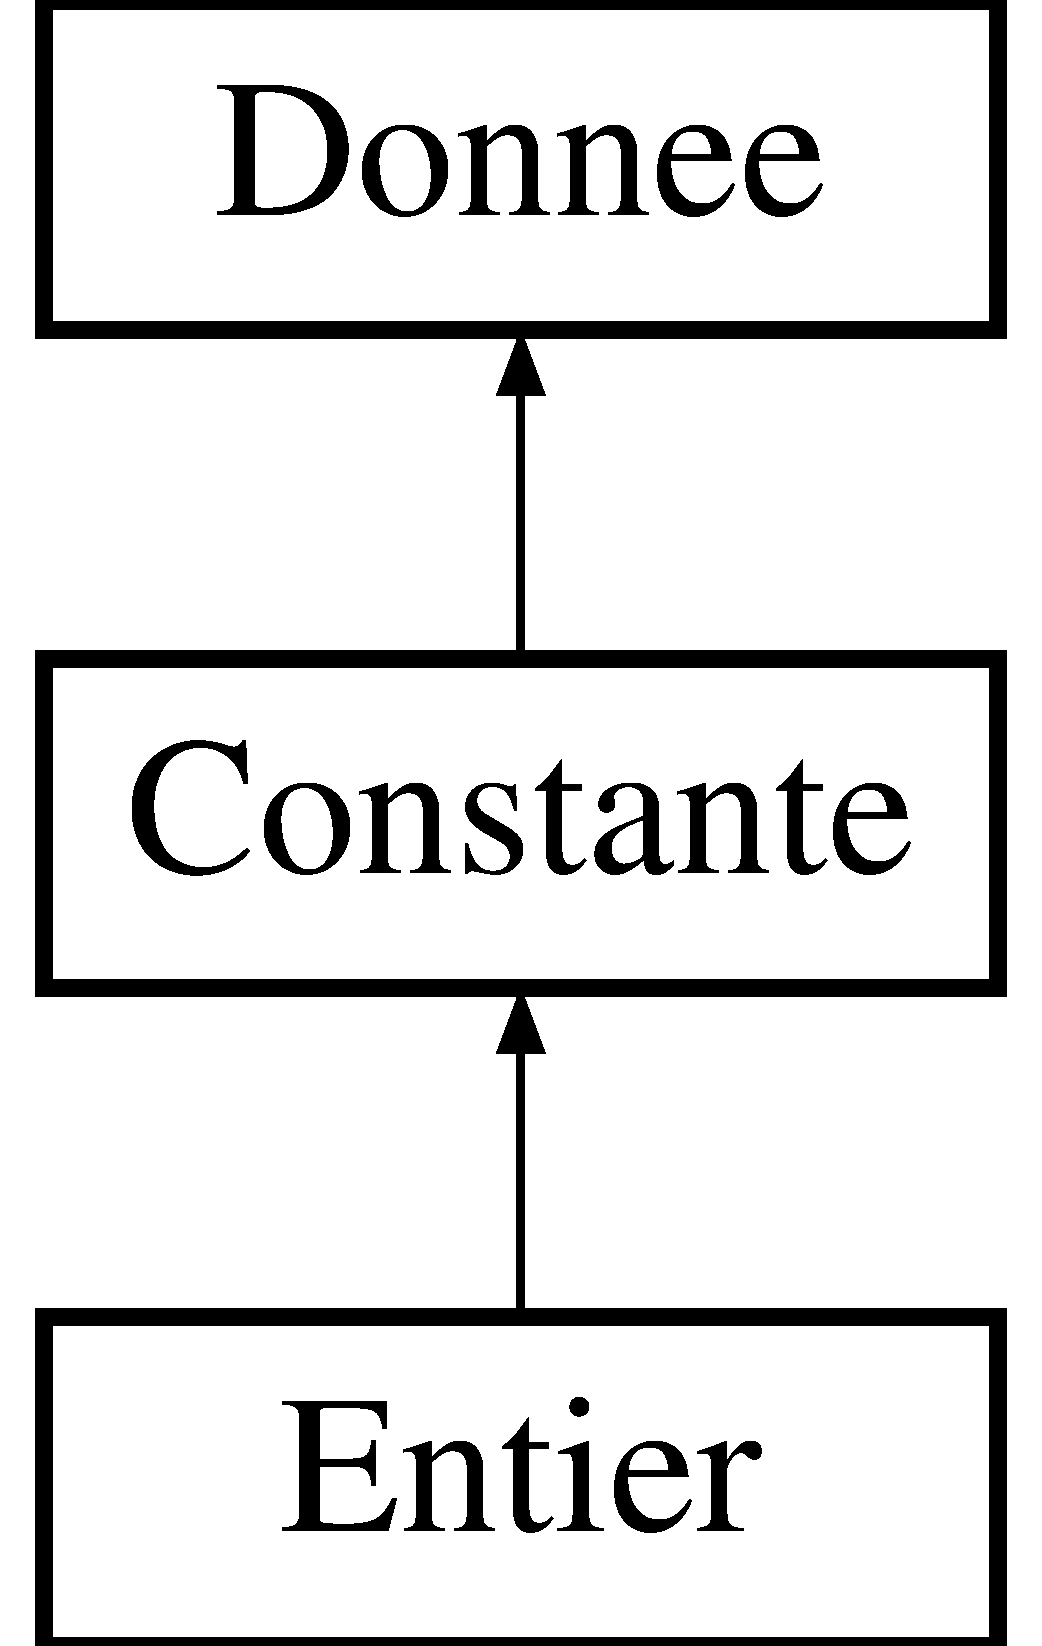
\includegraphics[height=3.000000cm]{class_entier}
\end{center}
\end{figure}
\subsection*{Fonctions membres publiques}
\begin{DoxyCompactItemize}
\item 
\hyperlink{class_entier_ab7343e7337fe0f74b26a370bd60e83fd}{Entier} (int val=0)
\begin{DoxyCompactList}\small\item\em Constructeur d'entier � partir d'un int. \end{DoxyCompactList}\item 
\hypertarget{class_entier_a2b243303497639116f0934b4adb065ae}{\hyperlink{class_entier_a2b243303497639116f0934b4adb065ae}{Entier} (const Q\-String \&a\-Q\-String=\char`\"{}0\char`\"{})}\label{class_entier_a2b243303497639116f0934b4adb065ae}

\begin{DoxyCompactList}\small\item\em Constructeur d'entier � partir d'une Q\-String. \end{DoxyCompactList}\item 
\hyperlink{class_entier_aaac9349e0d80cdab4e21701356d6268e}{Entier} (const \hyperlink{class_entier}{Entier} $\ast$a\-Entier)
\begin{DoxyCompactList}\small\item\em Constructeur de recopie. \end{DoxyCompactList}\item 
\hyperlink{class_entier_a158e9e75f76ddc9ecac74a26c192be65}{Entier} (const \hyperlink{class_reel}{Reel} $\ast$a\-Reel)
\begin{DoxyCompactList}\small\item\em Constructeur d'entier � partir de reel. \end{DoxyCompactList}\item 
\hyperlink{class_entier_aedf6d32377e1b4d190eb84590ea49c17}{Entier} (const \hyperlink{class_rationnel}{Rationnel} $\ast$a\-Rationnel)
\begin{DoxyCompactList}\small\item\em Constructeur d'entier � partir de rationnel. \end{DoxyCompactList}\item 
\hyperlink{class_entier_a891d9ad01b50f5fa0e310c58e18b16b3}{Entier} (const \hyperlink{class_complexe}{Complexe} $\ast$a\-Complexe)
\begin{DoxyCompactList}\small\item\em Constructeur d'entier � partir de complexe. \end{DoxyCompactList}\item 
virtual Q\-String \hyperlink{class_entier_ad3603b763e1d76b38fb2bceb883c8c89}{to\-Q\-String} () const 
\begin{DoxyCompactList}\small\item\em M�thode permettant d'obtenir l'objet sous la forme d'une Qstring. \end{DoxyCompactList}\item 
\hyperlink{class_entier}{Entier} $\ast$ \hyperlink{class_entier_a3a796ec0bc75a4bcae44fb6eea67cc10}{sign} ()
\begin{DoxyCompactList}\small\item\em Retourne un \hyperlink{class_entier}{Entier} ayant les memes valeurs mais avec le signe invers� \end{DoxyCompactList}\item 
int \hyperlink{class_entier_afe38ee7f81afc3c88a2c774ff0af2bcd}{get\-Valeur} () const 
\begin{DoxyCompactList}\small\item\em Acccesseur � la valeur. \end{DoxyCompactList}\item 
void \hyperlink{class_entier_a0f32791080ea409e112ce2893e9242cd}{set\-Valeur} (int a\-Valeur)
\begin{DoxyCompactList}\small\item\em Modificateur de valeur. \end{DoxyCompactList}\item 
\hyperlink{class_donnee}{Donnee} $\ast$ \hyperlink{class_entier_a1bcc1af417fd36f62bab9808f8fe6632}{operator+} (\hyperlink{class_donnee}{Donnee} $\ast$t)
\begin{DoxyCompactList}\small\item\em Operateur +. \end{DoxyCompactList}\item 
\hyperlink{class_donnee}{Donnee} $\ast$ \hyperlink{class_entier_a7253903447c5e1922c80e90af4e50e7f}{operator/} (\hyperlink{class_donnee}{Donnee} $\ast$t)
\begin{DoxyCompactList}\small\item\em Operateur /. \end{DoxyCompactList}\item 
\hyperlink{class_donnee}{Donnee} $\ast$ \hyperlink{class_entier_a3cd7bc09aaa5a9aa94fb868ef90c3cfa}{operator$\ast$} (\hyperlink{class_donnee}{Donnee} $\ast$t)
\begin{DoxyCompactList}\small\item\em Operateur $\ast$. \end{DoxyCompactList}\item 
\hyperlink{class_donnee}{Donnee} $\ast$ \hyperlink{class_entier_a42b4d223e6deb8e59abf5554488ede16}{operator-\/} (\hyperlink{class_donnee}{Donnee} $\ast$t)
\begin{DoxyCompactList}\small\item\em Operateur -\/. \end{DoxyCompactList}\item 
\hypertarget{class_entier_a70e589bc0a3f0f6fdf08a6a7fc5470bd}{int {\bfseries facto} (int n)}\label{class_entier_a70e589bc0a3f0f6fdf08a6a7fc5470bd}

\item 
virtual \hyperlink{class_donnee}{Donnee} $\ast$ \hyperlink{class_entier_ad2ff142a939a6e22b69d3d3915ef0371}{puissance} (\hyperlink{class_donnee}{Donnee} $\ast$t)
\begin{DoxyCompactList}\small\item\em puissance \end{DoxyCompactList}\item 
virtual \hyperlink{class_donnee}{Donnee} $\ast$ \hyperlink{class_entier_a4da8411b9f00afe85cab5874eb44c02a}{mod} (\hyperlink{class_donnee}{Donnee} $\ast$t)
\begin{DoxyCompactList}\small\item\em mod \end{DoxyCompactList}\item 
virtual \hyperlink{class_donnee}{Donnee} $\ast$ \hyperlink{class_entier_ac95bc2f1d50e5b4a851625ed5678e8a8}{my\-Sin} (int type\-Angle)
\begin{DoxyCompactList}\small\item\em my\-Sin \end{DoxyCompactList}\item 
virtual \hyperlink{class_donnee}{Donnee} $\ast$ \hyperlink{class_entier_a54c679369d395d8e912ea5f19734e54a}{my\-Cos} (int type\-Angle)
\begin{DoxyCompactList}\small\item\em my\-Cos \end{DoxyCompactList}\item 
virtual \hyperlink{class_donnee}{Donnee} $\ast$ \hyperlink{class_entier_a0b9531ba9f783a3f5d800b5caaa11370}{my\-Tan} (int type\-Angle)
\begin{DoxyCompactList}\small\item\em my\-Tan \end{DoxyCompactList}\item 
virtual \hyperlink{class_donnee}{Donnee} $\ast$ \hyperlink{class_entier_a28fdbd55d1208bb97c971052a43e16a5}{my\-Sinh} (int type\-Angle)
\begin{DoxyCompactList}\small\item\em my\-Sinh \end{DoxyCompactList}\item 
virtual \hyperlink{class_donnee}{Donnee} $\ast$ \hyperlink{class_entier_a278a767d66e7db0e4020bcdffb7f4b49}{my\-Cosh} (int type\-Angle)
\begin{DoxyCompactList}\small\item\em my\-Cosh \end{DoxyCompactList}\item 
virtual \hyperlink{class_donnee}{Donnee} $\ast$ \hyperlink{class_entier_a6157a86c4c407d35f5fec5d226e4dc6e}{my\-Tanh} (int type\-Angle)
\begin{DoxyCompactList}\small\item\em my\-Tanh \end{DoxyCompactList}\item 
virtual \hyperlink{class_donnee}{Donnee} $\ast$ \hyperlink{class_entier_a90a4a540f85f4295123eee2315439d6b}{my\-Ln} ()
\begin{DoxyCompactList}\small\item\em my\-Ln \end{DoxyCompactList}\item 
virtual \hyperlink{class_donnee}{Donnee} $\ast$ \hyperlink{class_entier_a4f95567ebc7c915427a4a840c4feb0c9}{my\-Log} ()
\begin{DoxyCompactList}\small\item\em my\-Log \end{DoxyCompactList}\item 
virtual \hyperlink{class_donnee}{Donnee} $\ast$ \hyperlink{class_entier_aa195655fde681a4ab18acecd54fb6e2f}{my\-Inv} ()
\begin{DoxyCompactList}\small\item\em my\-Inv \end{DoxyCompactList}\item 
virtual \hyperlink{class_donnee}{Donnee} $\ast$ \hyperlink{class_entier_a8ccc00629d9d7588998e9443916c2cff}{my\-Sqrt} ()
\begin{DoxyCompactList}\small\item\em my\-Sqrt \end{DoxyCompactList}\item 
virtual \hyperlink{class_donnee}{Donnee} $\ast$ \hyperlink{class_entier_a5379013e91b1d33c3a733594f6ae1db9}{my\-Sqr} ()
\begin{DoxyCompactList}\small\item\em my\-Sqr \end{DoxyCompactList}\item 
virtual \hyperlink{class_donnee}{Donnee} $\ast$ \hyperlink{class_entier_a2024dd6554fd0c38ab8c8d0ba6cf9e54}{my\-Cube} ()
\begin{DoxyCompactList}\small\item\em my\-Cube \end{DoxyCompactList}\item 
virtual \hyperlink{class_donnee}{Donnee} $\ast$ \hyperlink{class_entier_a0c512c175d294c572d19169293d503d3}{my\-Fact} ()
\begin{DoxyCompactList}\small\item\em my\-Fact \end{DoxyCompactList}\item 
bool \hyperlink{class_entier_ad152cf4769e7806be51719146043bf9d}{is\-Zero} ()
\begin{DoxyCompactList}\small\item\em is\-Zero \end{DoxyCompactList}\item 
bool \hyperlink{class_entier_a5fb33d1ee09365cb12703cc2e0737841}{is\-Neg} ()
\begin{DoxyCompactList}\small\item\em is\-Neg \end{DoxyCompactList}\end{DoxyCompactItemize}


\subsection{Description détaillée}
Classe des rationnels h�ritant de \hyperlink{class_constante}{Constante}. 

Pour fonctionner cette classe encapsule un entier. Tout les op�rateurs sont �galements red�finit. 

\subsection{Documentation des constructeurs et destructeur}
\hypertarget{class_entier_ab7343e7337fe0f74b26a370bd60e83fd}{\index{Entier@{Entier}!Entier@{Entier}}
\index{Entier@{Entier}!Entier@{Entier}}
\subsubsection[{Entier}]{\setlength{\rightskip}{0pt plus 5cm}Entier\-::\-Entier (
\begin{DoxyParamCaption}
\item[{int}]{val = {\ttfamily 0}}
\end{DoxyParamCaption}
)\hspace{0.3cm}{\ttfamily [inline]}}}\label{class_entier_ab7343e7337fe0f74b26a370bd60e83fd}


Constructeur d'entier � partir d'un int. 

Constructeur par valeur \begin{DoxyVerb}   \param   val        pour initialiser la valeur\end{DoxyVerb}
 \hypertarget{class_entier_aaac9349e0d80cdab4e21701356d6268e}{\index{Entier@{Entier}!Entier@{Entier}}
\index{Entier@{Entier}!Entier@{Entier}}
\subsubsection[{Entier}]{\setlength{\rightskip}{0pt plus 5cm}Entier\-::\-Entier (
\begin{DoxyParamCaption}
\item[{const {\bf Entier} $\ast$}]{a\-Entier}
\end{DoxyParamCaption}
)\hspace{0.3cm}{\ttfamily [inline]}}}\label{class_entier_aaac9349e0d80cdab4e21701356d6268e}


Constructeur de recopie. 


\begin{DoxyParams}{Paramètres}
{\em a\-Entier} & Un pointeur vers un autre entier \\
\hline
\end{DoxyParams}
\hypertarget{class_entier_a158e9e75f76ddc9ecac74a26c192be65}{\index{Entier@{Entier}!Entier@{Entier}}
\index{Entier@{Entier}!Entier@{Entier}}
\subsubsection[{Entier}]{\setlength{\rightskip}{0pt plus 5cm}Entier\-::\-Entier (
\begin{DoxyParamCaption}
\item[{const {\bf Reel} $\ast$}]{a\-Reel}
\end{DoxyParamCaption}
)}}\label{class_entier_a158e9e75f76ddc9ecac74a26c192be65}


Constructeur d'entier � partir de reel. 

On effectue un cast en ajoutant + 0,5 pour avoir un arrondi et non une troncature \begin{DoxyVerb}   \param   aReel pointeur sur le reel qui sert de modele � la construction\end{DoxyVerb}
 \hypertarget{class_entier_aedf6d32377e1b4d190eb84590ea49c17}{\index{Entier@{Entier}!Entier@{Entier}}
\index{Entier@{Entier}!Entier@{Entier}}
\subsubsection[{Entier}]{\setlength{\rightskip}{0pt plus 5cm}Entier\-::\-Entier (
\begin{DoxyParamCaption}
\item[{const {\bf Rationnel} $\ast$}]{a\-Rationnel}
\end{DoxyParamCaption}
)}}\label{class_entier_aedf6d32377e1b4d190eb84590ea49c17}


Constructeur d'entier � partir de rationnel. 


\begin{DoxyParams}{Paramètres}
{\em a\-Reel} & pointeur sur le rationnel qui sert de modele � la construction \\
\hline
\end{DoxyParams}
\hypertarget{class_entier_a891d9ad01b50f5fa0e310c58e18b16b3}{\index{Entier@{Entier}!Entier@{Entier}}
\index{Entier@{Entier}!Entier@{Entier}}
\subsubsection[{Entier}]{\setlength{\rightskip}{0pt plus 5cm}Entier\-::\-Entier (
\begin{DoxyParamCaption}
\item[{const {\bf Complexe} $\ast$}]{a\-Complexe}
\end{DoxyParamCaption}
)}}\label{class_entier_a891d9ad01b50f5fa0e310c58e18b16b3}


Constructeur d'entier � partir de complexe. 


\begin{DoxyParams}{Paramètres}
{\em a\-Reel} & pointeur sur le complexe qui sert de modele � la construction \\
\hline
\end{DoxyParams}


\subsection{Documentation des fonctions membres}
\hypertarget{class_entier_afe38ee7f81afc3c88a2c774ff0af2bcd}{\index{Entier@{Entier}!get\-Valeur@{get\-Valeur}}
\index{get\-Valeur@{get\-Valeur}!Entier@{Entier}}
\subsubsection[{get\-Valeur}]{\setlength{\rightskip}{0pt plus 5cm}int Entier\-::get\-Valeur (
\begin{DoxyParamCaption}
{}
\end{DoxyParamCaption}
) const\hspace{0.3cm}{\ttfamily [inline]}}}\label{class_entier_afe38ee7f81afc3c88a2c774ff0af2bcd}


Acccesseur � la valeur. 

\begin{DoxyReturn}{Renvoie}
Elle retourne la valeur de l'\hyperlink{class_entier}{Entier} 
\end{DoxyReturn}
\hypertarget{class_entier_a5fb33d1ee09365cb12703cc2e0737841}{\index{Entier@{Entier}!is\-Neg@{is\-Neg}}
\index{is\-Neg@{is\-Neg}!Entier@{Entier}}
\subsubsection[{is\-Neg}]{\setlength{\rightskip}{0pt plus 5cm}bool Entier\-::is\-Neg (
\begin{DoxyParamCaption}
{}
\end{DoxyParamCaption}
)\hspace{0.3cm}{\ttfamily [inline]}, {\ttfamily [virtual]}}}\label{class_entier_a5fb33d1ee09365cb12703cc2e0737841}


is\-Neg 

Mathode permettant de savoir si la \hyperlink{class_donnee}{Donnee} est inferieure ou egale � 0 \begin{DoxyReturn}{Renvoie}
bool true si la \hyperlink{class_donnee}{Donnee} est inferieur ou egale � 0 
\end{DoxyReturn}


Implémente \hyperlink{class_donnee_a0efb324f0c2e0682b971c3692c46e7c3}{Donnee}.

\hypertarget{class_entier_ad152cf4769e7806be51719146043bf9d}{\index{Entier@{Entier}!is\-Zero@{is\-Zero}}
\index{is\-Zero@{is\-Zero}!Entier@{Entier}}
\subsubsection[{is\-Zero}]{\setlength{\rightskip}{0pt plus 5cm}bool Entier\-::is\-Zero (
\begin{DoxyParamCaption}
{}
\end{DoxyParamCaption}
)\hspace{0.3cm}{\ttfamily [inline]}, {\ttfamily [virtual]}}}\label{class_entier_ad152cf4769e7806be51719146043bf9d}


is\-Zero 

Mathode permettant de savoir si la \hyperlink{class_donnee}{Donnee} est egale � 0 \begin{DoxyReturn}{Renvoie}
bool true si la \hyperlink{class_donnee}{Donnee} est egale � 0 
\end{DoxyReturn}


Implémente \hyperlink{class_donnee_aad251e4148c791719d7d7bff18680611}{Donnee}.

\hypertarget{class_entier_a4da8411b9f00afe85cab5874eb44c02a}{\index{Entier@{Entier}!mod@{mod}}
\index{mod@{mod}!Entier@{Entier}}
\subsubsection[{mod}]{\setlength{\rightskip}{0pt plus 5cm}{\bf Donnee} $\ast$ Entier\-::mod (
\begin{DoxyParamCaption}
\item[{{\bf Donnee} $\ast$}]{t}
\end{DoxyParamCaption}
)\hspace{0.3cm}{\ttfamily [virtual]}}}\label{class_entier_a4da8411b9f00afe85cab5874eb44c02a}


mod 

Implementation de l'op�rateur binaire modulo (methode virtuelle dans la classe mere) 
\begin{DoxyParams}{Paramètres}
{\em Donnee$\ast$,\-:} & Pointeur sur une donnee \\
\hline
\end{DoxyParams}
\begin{DoxyReturn}{Renvoie}
Pointeur sur donnee, resultat de l'operation 
\end{DoxyReturn}


Implémente \hyperlink{class_donnee_a52ce1aa17ce2c613e98428f82e3f85b8}{Donnee}.

\hypertarget{class_entier_a54c679369d395d8e912ea5f19734e54a}{\index{Entier@{Entier}!my\-Cos@{my\-Cos}}
\index{my\-Cos@{my\-Cos}!Entier@{Entier}}
\subsubsection[{my\-Cos}]{\setlength{\rightskip}{0pt plus 5cm}{\bf Donnee} $\ast$ Entier\-::my\-Cos (
\begin{DoxyParamCaption}
\item[{int}]{type\-Angle}
\end{DoxyParamCaption}
)\hspace{0.3cm}{\ttfamily [virtual]}}}\label{class_entier_a54c679369d395d8e912ea5f19734e54a}


my\-Cos 

Implementation de l'op�rateur unaire cosinus (methode virtuelle dans la classe mere) 
\begin{DoxyParams}{Paramètres}
{\em type\-Angle} & \-: entier, 0 si utilisation des degres, 1 si utilisation des radians \\
\hline
\end{DoxyParams}
\begin{DoxyReturn}{Renvoie}
Pointeur sur donnee, resultat de l'operation 
\end{DoxyReturn}


Implémente \hyperlink{class_donnee_abd9a62bd6b7d189f50db350823e895c3}{Donnee}.

\hypertarget{class_entier_a278a767d66e7db0e4020bcdffb7f4b49}{\index{Entier@{Entier}!my\-Cosh@{my\-Cosh}}
\index{my\-Cosh@{my\-Cosh}!Entier@{Entier}}
\subsubsection[{my\-Cosh}]{\setlength{\rightskip}{0pt plus 5cm}{\bf Donnee} $\ast$ Entier\-::my\-Cosh (
\begin{DoxyParamCaption}
\item[{int}]{type\-Angle}
\end{DoxyParamCaption}
)\hspace{0.3cm}{\ttfamily [virtual]}}}\label{class_entier_a278a767d66e7db0e4020bcdffb7f4b49}


my\-Cosh 

Implementation de l'op�rateur unaire cosinush (methode virtuelle dans la classe mere) 
\begin{DoxyParams}{Paramètres}
{\em type\-Angle} & \-: entier, 0 si utilisation des degres, 1 si utilisation des radians \\
\hline
\end{DoxyParams}
\begin{DoxyReturn}{Renvoie}
Pointeur sur donnee, resultat de l'operation 
\end{DoxyReturn}


Implémente \hyperlink{class_donnee_afe9b3532677d394b4b596021b74b6d17}{Donnee}.

\hypertarget{class_entier_a2024dd6554fd0c38ab8c8d0ba6cf9e54}{\index{Entier@{Entier}!my\-Cube@{my\-Cube}}
\index{my\-Cube@{my\-Cube}!Entier@{Entier}}
\subsubsection[{my\-Cube}]{\setlength{\rightskip}{0pt plus 5cm}{\bf Donnee} $\ast$ Entier\-::my\-Cube (
\begin{DoxyParamCaption}
{}
\end{DoxyParamCaption}
)\hspace{0.3cm}{\ttfamily [virtual]}}}\label{class_entier_a2024dd6554fd0c38ab8c8d0ba6cf9e54}


my\-Cube 

Implementation de l'op�rateur unaire Cube (methode virtuelle dans la classe mere) \begin{DoxyReturn}{Renvoie}
Pointeur sur donnee, resultat de l'operation 
\end{DoxyReturn}


Implémente \hyperlink{class_donnee_a875c21efdd22695c7999cfeb52ce4b2a}{Donnee}.

\hypertarget{class_entier_a0c512c175d294c572d19169293d503d3}{\index{Entier@{Entier}!my\-Fact@{my\-Fact}}
\index{my\-Fact@{my\-Fact}!Entier@{Entier}}
\subsubsection[{my\-Fact}]{\setlength{\rightskip}{0pt plus 5cm}{\bf Donnee} $\ast$ Entier\-::my\-Fact (
\begin{DoxyParamCaption}
{}
\end{DoxyParamCaption}
)\hspace{0.3cm}{\ttfamily [virtual]}}}\label{class_entier_a0c512c175d294c572d19169293d503d3}


my\-Fact 

Implementation de l'op�rateur unaire fact (methode virtuelle dans la classe mere) \begin{DoxyReturn}{Renvoie}
Pointeur sur donnee, resultat de l'operation 
\end{DoxyReturn}


Implémente \hyperlink{class_donnee_a79a2a3f835e09d0ed1888800c595a715}{Donnee}.

\hypertarget{class_entier_aa195655fde681a4ab18acecd54fb6e2f}{\index{Entier@{Entier}!my\-Inv@{my\-Inv}}
\index{my\-Inv@{my\-Inv}!Entier@{Entier}}
\subsubsection[{my\-Inv}]{\setlength{\rightskip}{0pt plus 5cm}{\bf Donnee} $\ast$ Entier\-::my\-Inv (
\begin{DoxyParamCaption}
{}
\end{DoxyParamCaption}
)\hspace{0.3cm}{\ttfamily [virtual]}}}\label{class_entier_aa195655fde681a4ab18acecd54fb6e2f}


my\-Inv 

Implementation de l'op�rateur unaire inv (methode virtuelle dans la classe mere) \begin{DoxyReturn}{Renvoie}
Pointeur sur donnee, resultat de l'operation 
\end{DoxyReturn}


Implémente \hyperlink{class_donnee_ad84c463eb43d4b98bed081045160fea1}{Donnee}.

\hypertarget{class_entier_a90a4a540f85f4295123eee2315439d6b}{\index{Entier@{Entier}!my\-Ln@{my\-Ln}}
\index{my\-Ln@{my\-Ln}!Entier@{Entier}}
\subsubsection[{my\-Ln}]{\setlength{\rightskip}{0pt plus 5cm}{\bf Donnee} $\ast$ Entier\-::my\-Ln (
\begin{DoxyParamCaption}
{}
\end{DoxyParamCaption}
)\hspace{0.3cm}{\ttfamily [virtual]}}}\label{class_entier_a90a4a540f85f4295123eee2315439d6b}


my\-Ln 

Implementation de l'op�rateur unaire ln (methode virtuelle dans la classe mere) \begin{DoxyReturn}{Renvoie}
Pointeur sur donnee, resultat de l'operation 
\end{DoxyReturn}


Implémente \hyperlink{class_donnee_ac24ba41baf90eb99bcf91145c541780a}{Donnee}.

\hypertarget{class_entier_a4f95567ebc7c915427a4a840c4feb0c9}{\index{Entier@{Entier}!my\-Log@{my\-Log}}
\index{my\-Log@{my\-Log}!Entier@{Entier}}
\subsubsection[{my\-Log}]{\setlength{\rightskip}{0pt plus 5cm}{\bf Donnee} $\ast$ Entier\-::my\-Log (
\begin{DoxyParamCaption}
{}
\end{DoxyParamCaption}
)\hspace{0.3cm}{\ttfamily [virtual]}}}\label{class_entier_a4f95567ebc7c915427a4a840c4feb0c9}


my\-Log 

Implementation de l'op�rateur unaire log (methode virtuelle dans la classe mere) \begin{DoxyReturn}{Renvoie}
Pointeur sur donnee, resultat de l'operation 
\end{DoxyReturn}


Implémente \hyperlink{class_donnee_a7ac3f554be1fc579b02d9c877185cf50}{Donnee}.

\hypertarget{class_entier_ac95bc2f1d50e5b4a851625ed5678e8a8}{\index{Entier@{Entier}!my\-Sin@{my\-Sin}}
\index{my\-Sin@{my\-Sin}!Entier@{Entier}}
\subsubsection[{my\-Sin}]{\setlength{\rightskip}{0pt plus 5cm}{\bf Donnee} $\ast$ Entier\-::my\-Sin (
\begin{DoxyParamCaption}
\item[{int}]{type\-Angle}
\end{DoxyParamCaption}
)\hspace{0.3cm}{\ttfamily [virtual]}}}\label{class_entier_ac95bc2f1d50e5b4a851625ed5678e8a8}


my\-Sin 

Implementation de l'op�rateur unaire sinus (methode virtuelle dans la classe mere) 
\begin{DoxyParams}{Paramètres}
{\em type\-Angle} & \-: entier, 0 si utilisation des degres, 1 si utilisation des radians \\
\hline
\end{DoxyParams}
\begin{DoxyReturn}{Renvoie}
Pointeur sur donnee, resultat de l'operation 
\end{DoxyReturn}


Implémente \hyperlink{class_donnee_a86f71d87c3a69dc6dcede4b411d94043}{Donnee}.

\hypertarget{class_entier_a28fdbd55d1208bb97c971052a43e16a5}{\index{Entier@{Entier}!my\-Sinh@{my\-Sinh}}
\index{my\-Sinh@{my\-Sinh}!Entier@{Entier}}
\subsubsection[{my\-Sinh}]{\setlength{\rightskip}{0pt plus 5cm}{\bf Donnee} $\ast$ Entier\-::my\-Sinh (
\begin{DoxyParamCaption}
\item[{int}]{type\-Angle}
\end{DoxyParamCaption}
)\hspace{0.3cm}{\ttfamily [virtual]}}}\label{class_entier_a28fdbd55d1208bb97c971052a43e16a5}


my\-Sinh 

Implementation de l'op�rateur unaire sinush (methode virtuelle dans la classe mere) 
\begin{DoxyParams}{Paramètres}
{\em type\-Angle} & \-: entier, 0 si utilisation des degres, 1 si utilisation des radians \\
\hline
\end{DoxyParams}
\begin{DoxyReturn}{Renvoie}
Pointeur sur donnee, resultat de l'operation 
\end{DoxyReturn}


Implémente \hyperlink{class_donnee_af3c408a3fda8f24ee70f34fd8688fe63}{Donnee}.

\hypertarget{class_entier_a5379013e91b1d33c3a733594f6ae1db9}{\index{Entier@{Entier}!my\-Sqr@{my\-Sqr}}
\index{my\-Sqr@{my\-Sqr}!Entier@{Entier}}
\subsubsection[{my\-Sqr}]{\setlength{\rightskip}{0pt plus 5cm}{\bf Donnee} $\ast$ Entier\-::my\-Sqr (
\begin{DoxyParamCaption}
{}
\end{DoxyParamCaption}
)\hspace{0.3cm}{\ttfamily [virtual]}}}\label{class_entier_a5379013e91b1d33c3a733594f6ae1db9}


my\-Sqr 

Implementation de l'op�rateur unaire sqr (methode virtuelle dans la classe mere) \begin{DoxyReturn}{Renvoie}
Pointeur sur donnee, resultat de l'operation 
\end{DoxyReturn}


Implémente \hyperlink{class_donnee_a708281bf8ddb3f6c33a100b3db925901}{Donnee}.

\hypertarget{class_entier_a8ccc00629d9d7588998e9443916c2cff}{\index{Entier@{Entier}!my\-Sqrt@{my\-Sqrt}}
\index{my\-Sqrt@{my\-Sqrt}!Entier@{Entier}}
\subsubsection[{my\-Sqrt}]{\setlength{\rightskip}{0pt plus 5cm}{\bf Donnee} $\ast$ Entier\-::my\-Sqrt (
\begin{DoxyParamCaption}
{}
\end{DoxyParamCaption}
)\hspace{0.3cm}{\ttfamily [virtual]}}}\label{class_entier_a8ccc00629d9d7588998e9443916c2cff}


my\-Sqrt 

Implementation de l'op�rateur unaire sqrt (methode virtuelle dans la classe mere) \begin{DoxyReturn}{Renvoie}
Pointeur sur donnee, resultat de l'operation 
\end{DoxyReturn}


Implémente \hyperlink{class_donnee_a07484cd79bc071fbfc48ace5bcd94e8f}{Donnee}.

\hypertarget{class_entier_a0b9531ba9f783a3f5d800b5caaa11370}{\index{Entier@{Entier}!my\-Tan@{my\-Tan}}
\index{my\-Tan@{my\-Tan}!Entier@{Entier}}
\subsubsection[{my\-Tan}]{\setlength{\rightskip}{0pt plus 5cm}{\bf Donnee} $\ast$ Entier\-::my\-Tan (
\begin{DoxyParamCaption}
\item[{int}]{type\-Angle}
\end{DoxyParamCaption}
)\hspace{0.3cm}{\ttfamily [virtual]}}}\label{class_entier_a0b9531ba9f783a3f5d800b5caaa11370}


my\-Tan 

Implementation de l'op�rateur unaire tangente (methode virtuelle dans la classe mere) 
\begin{DoxyParams}{Paramètres}
{\em type\-Angle} & \-: entier, 0 si utilisation des degres, 1 si utilisation des radians \\
\hline
\end{DoxyParams}
\begin{DoxyReturn}{Renvoie}
Pointeur sur donnee, resultat de l'operation 
\end{DoxyReturn}


Implémente \hyperlink{class_donnee_ad3b4b9d20c0693915d9c17b528bed4d8}{Donnee}.

\hypertarget{class_entier_a6157a86c4c407d35f5fec5d226e4dc6e}{\index{Entier@{Entier}!my\-Tanh@{my\-Tanh}}
\index{my\-Tanh@{my\-Tanh}!Entier@{Entier}}
\subsubsection[{my\-Tanh}]{\setlength{\rightskip}{0pt plus 5cm}{\bf Donnee} $\ast$ Entier\-::my\-Tanh (
\begin{DoxyParamCaption}
\item[{int}]{type\-Angle}
\end{DoxyParamCaption}
)\hspace{0.3cm}{\ttfamily [virtual]}}}\label{class_entier_a6157a86c4c407d35f5fec5d226e4dc6e}


my\-Tanh 

Implementation de l'op�rateur unaire tangenteh (methode virtuelle dans la classe mere) 
\begin{DoxyParams}{Paramètres}
{\em type\-Angle} & \-: entier, 0 si utilisation des degres, 1 si utilisation des radians \\
\hline
\end{DoxyParams}
\begin{DoxyReturn}{Renvoie}
Pointeur sur donnee, resultat de l'operation 
\end{DoxyReturn}


Implémente \hyperlink{class_donnee_a20a90ca79d91dc75ea01cc3842b0e6dd}{Donnee}.

\hypertarget{class_entier_a3cd7bc09aaa5a9aa94fb868ef90c3cfa}{\index{Entier@{Entier}!operator$\ast$@{operator$\ast$}}
\index{operator$\ast$@{operator$\ast$}!Entier@{Entier}}
\subsubsection[{operator$\ast$}]{\setlength{\rightskip}{0pt plus 5cm}{\bf Donnee} $\ast$ Entier\-::operator$\ast$ (
\begin{DoxyParamCaption}
\item[{{\bf Donnee} $\ast$}]{t}
\end{DoxyParamCaption}
)\hspace{0.3cm}{\ttfamily [virtual]}}}\label{class_entier_a3cd7bc09aaa5a9aa94fb868ef90c3cfa}


Operateur $\ast$. 

Implementation de l'op�rateur binaire $\ast$ (methode virtuelle dans la classe mere) 
\begin{DoxyParams}{Paramètres}
{\em t} & \-: Pointeur sur un type \\
\hline
\end{DoxyParams}
\begin{DoxyReturn}{Renvoie}
Pointeur sur type, resultat de l'operation 
\end{DoxyReturn}


Implémente \hyperlink{class_donnee_ae655c41f021de91a35d652a8519d4eb2}{Donnee}.

\hypertarget{class_entier_a1bcc1af417fd36f62bab9808f8fe6632}{\index{Entier@{Entier}!operator+@{operator+}}
\index{operator+@{operator+}!Entier@{Entier}}
\subsubsection[{operator+}]{\setlength{\rightskip}{0pt plus 5cm}{\bf Donnee} $\ast$ Entier\-::operator+ (
\begin{DoxyParamCaption}
\item[{{\bf Donnee} $\ast$}]{t}
\end{DoxyParamCaption}
)\hspace{0.3cm}{\ttfamily [virtual]}}}\label{class_entier_a1bcc1af417fd36f62bab9808f8fe6632}


Operateur +. 

Implementation de l'op�rateur binaire + (methode virtuelle dans la classe mere) 
\begin{DoxyParams}{Paramètres}
{\em t} & \-: Pointeur sur un type \\
\hline
\end{DoxyParams}
\begin{DoxyReturn}{Renvoie}
Pointeur sur type, resultat de l'operation 
\end{DoxyReturn}


Implémente \hyperlink{class_donnee_acda2976724adeef2233e7077953c1a9a}{Donnee}.

\hypertarget{class_entier_a42b4d223e6deb8e59abf5554488ede16}{\index{Entier@{Entier}!operator-\/@{operator-\/}}
\index{operator-\/@{operator-\/}!Entier@{Entier}}
\subsubsection[{operator-\/}]{\setlength{\rightskip}{0pt plus 5cm}{\bf Donnee} $\ast$ Entier\-::operator-\/ (
\begin{DoxyParamCaption}
\item[{{\bf Donnee} $\ast$}]{t}
\end{DoxyParamCaption}
)\hspace{0.3cm}{\ttfamily [virtual]}}}\label{class_entier_a42b4d223e6deb8e59abf5554488ede16}


Operateur -\/. 

Implementation de l'op�rateur binaire -\/ (methode virtuelle dans la classe mere) 
\begin{DoxyParams}{Paramètres}
{\em t} & \-: Pointeur sur un type \\
\hline
\end{DoxyParams}
\begin{DoxyReturn}{Renvoie}
Pointeur sur type, resultat de l'operation 
\end{DoxyReturn}


Implémente \hyperlink{class_donnee_a053ea4f3f00b6e0a73b4ea453adca1be}{Donnee}.

\hypertarget{class_entier_a7253903447c5e1922c80e90af4e50e7f}{\index{Entier@{Entier}!operator/@{operator/}}
\index{operator/@{operator/}!Entier@{Entier}}
\subsubsection[{operator/}]{\setlength{\rightskip}{0pt plus 5cm}{\bf Donnee} $\ast$ Entier\-::operator/ (
\begin{DoxyParamCaption}
\item[{{\bf Donnee} $\ast$}]{t}
\end{DoxyParamCaption}
)\hspace{0.3cm}{\ttfamily [virtual]}}}\label{class_entier_a7253903447c5e1922c80e90af4e50e7f}


Operateur /. 

Implementation de l'op�rateur binaire / (methode virtuelle dans la classe mere) 
\begin{DoxyParams}{Paramètres}
{\em t} & \-: Pointeur sur un type \\
\hline
\end{DoxyParams}
\begin{DoxyReturn}{Renvoie}
Pointeur sur type, resultat de l'operation 
\end{DoxyReturn}


Implémente \hyperlink{class_donnee_abc63ffa0d62612446435ff1eca34344b}{Donnee}.

\hypertarget{class_entier_ad2ff142a939a6e22b69d3d3915ef0371}{\index{Entier@{Entier}!puissance@{puissance}}
\index{puissance@{puissance}!Entier@{Entier}}
\subsubsection[{puissance}]{\setlength{\rightskip}{0pt plus 5cm}{\bf Donnee} $\ast$ Entier\-::puissance (
\begin{DoxyParamCaption}
\item[{{\bf Donnee} $\ast$}]{t}
\end{DoxyParamCaption}
)\hspace{0.3cm}{\ttfamily [virtual]}}}\label{class_entier_ad2ff142a939a6e22b69d3d3915ef0371}


puissance 

Implementation de l'op�rateur binaire puissance (methode virtuelle dans la classe mere) 
\begin{DoxyParams}{Paramètres}
{\em Donnee$\ast$,\-:} & Pointeur sur une donnee \\
\hline
\end{DoxyParams}
\begin{DoxyReturn}{Renvoie}
Pointeur sur donnee, resultat de l'operation 
\end{DoxyReturn}


Implémente \hyperlink{class_donnee_af25f76885c91b1a497023c9dd2231990}{Donnee}.

\hypertarget{class_entier_a0f32791080ea409e112ce2893e9242cd}{\index{Entier@{Entier}!set\-Valeur@{set\-Valeur}}
\index{set\-Valeur@{set\-Valeur}!Entier@{Entier}}
\subsubsection[{set\-Valeur}]{\setlength{\rightskip}{0pt plus 5cm}void Entier\-::set\-Valeur (
\begin{DoxyParamCaption}
\item[{int}]{a\-Valeur}
\end{DoxyParamCaption}
)\hspace{0.3cm}{\ttfamily [inline]}}}\label{class_entier_a0f32791080ea409e112ce2893e9242cd}


Modificateur de valeur. 


\begin{DoxyParams}{Paramètres}
{\em a\-Valeur} & La nouvelle valeur de l'entier \\
\hline
\end{DoxyParams}
\hypertarget{class_entier_a3a796ec0bc75a4bcae44fb6eea67cc10}{\index{Entier@{Entier}!sign@{sign}}
\index{sign@{sign}!Entier@{Entier}}
\subsubsection[{sign}]{\setlength{\rightskip}{0pt plus 5cm}{\bf Entier}$\ast$ Entier\-::sign (
\begin{DoxyParamCaption}
{}
\end{DoxyParamCaption}
)\hspace{0.3cm}{\ttfamily [inline]}, {\ttfamily [virtual]}}}\label{class_entier_a3a796ec0bc75a4bcae44fb6eea67cc10}


Retourne un \hyperlink{class_entier}{Entier} ayant les memes valeurs mais avec le signe invers� 

Pour fonctionner, elle utilise le constructeur \hyperlink{class_entier}{Entier} par valeur \begin{DoxyVerb}   \return   Elle retourne le rationnel construit (=-this).\end{DoxyVerb}
 

Implémente \hyperlink{class_constante_a3d218a44f46136c5d69f04821f100953}{Constante}.

\hypertarget{class_entier_ad3603b763e1d76b38fb2bceb883c8c89}{\index{Entier@{Entier}!to\-Q\-String@{to\-Q\-String}}
\index{to\-Q\-String@{to\-Q\-String}!Entier@{Entier}}
\subsubsection[{to\-Q\-String}]{\setlength{\rightskip}{0pt plus 5cm}Q\-String Entier\-::to\-Q\-String (
\begin{DoxyParamCaption}
{}
\end{DoxyParamCaption}
) const\hspace{0.3cm}{\ttfamily [virtual]}}}\label{class_entier_ad3603b763e1d76b38fb2bceb883c8c89}


M�thode permettant d'obtenir l'objet sous la forme d'une Qstring. 

\begin{DoxyReturn}{Renvoie}
Elle retourne un Qstring tel qu'un entier puisse etre construit � partir de �a, ou affich�. 
\end{DoxyReturn}


Implémente \hyperlink{class_donnee_ad96590e462f8db33aefca28ba8e31e52}{Donnee}.



La documentation de cette classe a été générée à partir des fichiers suivants \-:\begin{DoxyCompactItemize}
\item 
\hyperlink{entier_8h}{entier.\-h}\item 
entier.\-cpp\end{DoxyCompactItemize}

\hypertarget{class_exception_coo_coo}{\section{Référence de la classe Exception\-Coo\-Coo}
\label{class_exception_coo_coo}\index{Exception\-Coo\-Coo@{Exception\-Coo\-Coo}}
}


Classe d'exception.  




{\ttfamily \#include $<$exception\-Coo\-Coo.\-h$>$}

\subsection*{Fonctions membres publiques}
\begin{DoxyCompactItemize}
\item 
\hyperlink{class_exception_coo_coo_abc4fda1d887ebf8167aa292b22006cbf}{Exception\-Coo\-Coo} (const char $\ast$s=\char`\"{}\char`\"{})
\begin{DoxyCompactList}\small\item\em Constructeur. \end{DoxyCompactList}\item 
const char $\ast$ \hyperlink{class_exception_coo_coo_a146a13e09e5071f4d9461b11701ba5aa}{Get\-Infos} () const   throw ()
\begin{DoxyCompactList}\small\item\em Get\-Infos. \end{DoxyCompactList}\item 
\hypertarget{class_exception_coo_coo_a4da74063dcd709e6bf23b4d77275a362}{\hyperlink{class_exception_coo_coo_a4da74063dcd709e6bf23b4d77275a362}{$\sim$\-Exception\-Coo\-Coo} ()  throw ()}\label{class_exception_coo_coo_a4da74063dcd709e6bf23b4d77275a362}

\begin{DoxyCompactList}\small\item\em Destructeur. \end{DoxyCompactList}\end{DoxyCompactItemize}


\subsection{Description détaillée}
Classe d'exception. 

Derive de std\-::exception 

\subsection{Documentation des constructeurs et destructeur}
\hypertarget{class_exception_coo_coo_abc4fda1d887ebf8167aa292b22006cbf}{\index{Exception\-Coo\-Coo@{Exception\-Coo\-Coo}!Exception\-Coo\-Coo@{Exception\-Coo\-Coo}}
\index{Exception\-Coo\-Coo@{Exception\-Coo\-Coo}!ExceptionCooCoo@{Exception\-Coo\-Coo}}
\subsubsection[{Exception\-Coo\-Coo}]{\setlength{\rightskip}{0pt plus 5cm}Exception\-Coo\-Coo\-::\-Exception\-Coo\-Coo (
\begin{DoxyParamCaption}
\item[{const char $\ast$}]{s = {\ttfamily \char`\"{}\char`\"{}}}
\end{DoxyParamCaption}
)\hspace{0.3cm}{\ttfamily [inline]}}}\label{class_exception_coo_coo_abc4fda1d887ebf8167aa292b22006cbf}


Constructeur. 

Construit une exception a partir d'une chaine de caracteres 

\subsection{Documentation des fonctions membres}
\hypertarget{class_exception_coo_coo_a146a13e09e5071f4d9461b11701ba5aa}{\index{Exception\-Coo\-Coo@{Exception\-Coo\-Coo}!Get\-Infos@{Get\-Infos}}
\index{Get\-Infos@{Get\-Infos}!ExceptionCooCoo@{Exception\-Coo\-Coo}}
\subsubsection[{Get\-Infos}]{\setlength{\rightskip}{0pt plus 5cm}const char$\ast$ Exception\-Coo\-Coo\-::\-Get\-Infos (
\begin{DoxyParamCaption}
{}
\end{DoxyParamCaption}
) const  throw ()\hspace{0.3cm}{\ttfamily [inline]}}}\label{class_exception_coo_coo_a146a13e09e5071f4d9461b11701ba5aa}


Get\-Infos. 

Permet d'en savoir plus sur la cause de l'erreur 

La documentation de cette classe a été générée à partir du fichier suivant \-:\begin{DoxyCompactItemize}
\item 
\hyperlink{exception_coo_coo_8h}{exception\-Coo\-Coo.\-h}\end{DoxyCompactItemize}

\hypertarget{class_fabrique_donnee}{\section{Fabrique\-Donnee Class Reference}
\label{class_fabrique_donnee}\index{Fabrique\-Donnee@{Fabrique\-Donnee}}
}


Classe fabrique de donnee.  




{\ttfamily \#include $<$fabriquedonnee.\-h$>$}

\subsection*{Public Member Functions}
\begin{DoxyCompactItemize}
\item 
\hyperlink{class_donnee}{Donnee} $\ast$ \hyperlink{class_fabrique_donnee_a134aaa24758a0d8fc8a013c86b43aba2}{creer\-Donnee} (const Q\-String \&terme)
\begin{DoxyCompactList}\small\item\em creer\-Donnee Methode permettant de creer une nouvelle \hyperlink{class_donnee}{Donnee}, teste le type represente par la chaine et cree la \hyperlink{class_donnee}{Donnee} correspondante en appellant le constructeur de son type \end{DoxyCompactList}\item 
\hyperlink{class_donnee}{Donnee} $\ast$ \hyperlink{class_fabrique_donnee_a6598e4d4d69047836b5f079dc8684636}{creer\-Donnee} (const \hyperlink{class_donnee}{Donnee} $\ast$donnee\-Depart, int type\-Souhaite, int complexe)
\begin{DoxyCompactList}\small\item\em creer\-Donnee Methode surcharg�e permettant de convertir des objets d'une classe fille de \hyperlink{class_donnee}{Donnee} en une autre \end{DoxyCompactList}\end{DoxyCompactItemize}
\subsection*{Static Public Member Functions}
\begin{DoxyCompactItemize}
\item 
static \hyperlink{class_fabrique_donnee}{Fabrique\-Donnee} $\ast$ \hyperlink{class_fabrique_donnee_a9b14e807a2702c4a4c0a607d6b337db7}{get\-Instance} ()
\begin{DoxyCompactList}\small\item\em get\-Instance Methode retournant l'instance unique de la classe Fabrique\-Donne \end{DoxyCompactList}\item 
\hypertarget{class_fabrique_donnee_a4ca786abc0119d5e69d054632398bfa3}{static void \hyperlink{class_fabrique_donnee_a4ca786abc0119d5e69d054632398bfa3}{libere\-Instance} ()}\label{class_fabrique_donnee_a4ca786abc0119d5e69d054632398bfa3}

\begin{DoxyCompactList}\small\item\em libere\-Instance Methode liberant l'instance unique de la classe \end{DoxyCompactList}\end{DoxyCompactItemize}


\subsection{Detailed Description}
Classe fabrique de donnee. 

La classe est un singleton, implementation du design pattern Factory 

\subsection{Member Function Documentation}
\hypertarget{class_fabrique_donnee_a134aaa24758a0d8fc8a013c86b43aba2}{\index{Fabrique\-Donnee@{Fabrique\-Donnee}!creer\-Donnee@{creer\-Donnee}}
\index{creer\-Donnee@{creer\-Donnee}!FabriqueDonnee@{Fabrique\-Donnee}}
\subsubsection[{creer\-Donnee}]{\setlength{\rightskip}{0pt plus 5cm}{\bf Donnee} $\ast$ Fabrique\-Donnee\-::creer\-Donnee (
\begin{DoxyParamCaption}
\item[{const Q\-String \&}]{terme}
\end{DoxyParamCaption}
)}}\label{class_fabrique_donnee_a134aaa24758a0d8fc8a013c86b43aba2}


creer\-Donnee Methode permettant de creer une nouvelle \hyperlink{class_donnee}{Donnee}, teste le type represente par la chaine et cree la \hyperlink{class_donnee}{Donnee} correspondante en appellant le constructeur de son type 


\begin{DoxyParams}{Parameters}
{\em terme,chaine} & de caractere source \\
\hline
\end{DoxyParams}
\begin{DoxyReturn}{Returns}
Pointeur sur \hyperlink{class_donnee}{Donnee}, nouvelle \hyperlink{class_donnee}{Donnee} cree 
\end{DoxyReturn}
\hypertarget{class_fabrique_donnee_a6598e4d4d69047836b5f079dc8684636}{\index{Fabrique\-Donnee@{Fabrique\-Donnee}!creer\-Donnee@{creer\-Donnee}}
\index{creer\-Donnee@{creer\-Donnee}!FabriqueDonnee@{Fabrique\-Donnee}}
\subsubsection[{creer\-Donnee}]{\setlength{\rightskip}{0pt plus 5cm}{\bf Donnee} $\ast$ Fabrique\-Donnee\-::creer\-Donnee (
\begin{DoxyParamCaption}
\item[{const {\bf Donnee} $\ast$}]{donnee\-Depart, }
\item[{int}]{type\-Souhaite, }
\item[{int}]{complexe}
\end{DoxyParamCaption}
)}}\label{class_fabrique_donnee_a6598e4d4d69047836b5f079dc8684636}


creer\-Donnee Methode surcharg�e permettant de convertir des objets d'une classe fille de \hyperlink{class_donnee}{Donnee} en une autre 


\begin{DoxyParams}{Parameters}
{\em donnee\-Depart} & pointeur const de \hyperlink{class_donnee}{Donnee}, la donn�e que l'on veut convertir \\
\hline
{\em type\-Souhaite} & entier indiquant le type de retour souhait� (0=reel, 1=rationnel, 2=reel) \\
\hline
{\em complexe} & entier indiquant si le retour doit �tre complexe ou non \\
\hline
\end{DoxyParams}
\begin{DoxyReturn}{Returns}
Pointeur sur \hyperlink{class_donnee}{Donnee}, nouvelle \hyperlink{class_donnee}{Donnee} cree 
\end{DoxyReturn}
\hypertarget{class_fabrique_donnee_a9b14e807a2702c4a4c0a607d6b337db7}{\index{Fabrique\-Donnee@{Fabrique\-Donnee}!get\-Instance@{get\-Instance}}
\index{get\-Instance@{get\-Instance}!FabriqueDonnee@{Fabrique\-Donnee}}
\subsubsection[{get\-Instance}]{\setlength{\rightskip}{0pt plus 5cm}{\bf Fabrique\-Donnee} $\ast$ Fabrique\-Donnee\-::get\-Instance (
\begin{DoxyParamCaption}
{}
\end{DoxyParamCaption}
)\hspace{0.3cm}{\ttfamily [static]}}}\label{class_fabrique_donnee_a9b14e807a2702c4a4c0a607d6b337db7}


get\-Instance Methode retournant l'instance unique de la classe Fabrique\-Donne 

\begin{DoxyReturn}{Returns}
Instance unique de la classe 
\end{DoxyReturn}


The documentation for this class was generated from the following files\-:\begin{DoxyCompactItemize}
\item 
fabriquedonnee.\-h\item 
fabriquedonnee.\-cpp\end{DoxyCompactItemize}

\hypertarget{class_gardien}{\section{Gardien Class Reference}
\label{class_gardien}\index{Gardien@{Gardien}}
}


Classe de \hyperlink{class_gardien}{Gardien} La classe permet de sauvegarder les etats d'une pile, dans le but de pouvoir les restaurer Partie du design pattern \char`\"{}\-Memento\char`\"{}.  




{\ttfamily \#include $<$memento.\-h$>$}

\subsection*{Public Member Functions}
\begin{DoxyCompactItemize}
\item 
\hyperlink{class_gardien_aab8526f0f25e03d4cb1babbc1aa6d09e}{Gardien} ()
\begin{DoxyCompactList}\small\item\em Constructeur. \end{DoxyCompactList}\item 
\hypertarget{class_gardien_afef6202d924fef9d882bb40dfc4ac9fb}{\hyperlink{class_gardien_afef6202d924fef9d882bb40dfc4ac9fb}{$\sim$\-Gardien} ()}\label{class_gardien_afef6202d924fef9d882bb40dfc4ac9fb}

\begin{DoxyCompactList}\small\item\em Destructeur. \end{DoxyCompactList}\item 
void \hyperlink{class_gardien_ab152ac41cab1dc3f3a1dc0f143a54aa3}{add\-Memento} (\hyperlink{class_pile}{Pile} $\ast$a\-Pile)
\begin{DoxyCompactList}\small\item\em add\-Memento Permet d'ajouter un etat dans le vecteur de pile \end{DoxyCompactList}\item 
\hyperlink{class_pile}{Pile} $\ast$ \hyperlink{class_gardien_ac0145da9f36f0dbf7a6894723249dd1f}{undo} ()
\begin{DoxyCompactList}\small\item\em Undo Permet de restaurer l'etat precedent. \end{DoxyCompactList}\item 
\hyperlink{class_pile}{Pile} $\ast$ \hyperlink{class_gardien_a9fa7f0b6196b9b551b9ff9506d9ef8bf}{redo} ()
\begin{DoxyCompactList}\small\item\em Redo Permet de restaurer l'etat suivant. \end{DoxyCompactList}\end{DoxyCompactItemize}


\subsection{Detailed Description}
Classe de \hyperlink{class_gardien}{Gardien} La classe permet de sauvegarder les etats d'une pile, dans le but de pouvoir les restaurer Partie du design pattern \char`\"{}\-Memento\char`\"{}. 

\subsection{Constructor \& Destructor Documentation}
\hypertarget{class_gardien_aab8526f0f25e03d4cb1babbc1aa6d09e}{\index{Gardien@{Gardien}!Gardien@{Gardien}}
\index{Gardien@{Gardien}!Gardien@{Gardien}}
\subsubsection[{Gardien}]{\setlength{\rightskip}{0pt plus 5cm}Gardien\-::\-Gardien (
\begin{DoxyParamCaption}
{}
\end{DoxyParamCaption}
)\hspace{0.3cm}{\ttfamily [inline]}}}\label{class_gardien_aab8526f0f25e03d4cb1babbc1aa6d09e}


Constructeur. 

Construit un gardien 

\subsection{Member Function Documentation}
\hypertarget{class_gardien_ab152ac41cab1dc3f3a1dc0f143a54aa3}{\index{Gardien@{Gardien}!add\-Memento@{add\-Memento}}
\index{add\-Memento@{add\-Memento}!Gardien@{Gardien}}
\subsubsection[{add\-Memento}]{\setlength{\rightskip}{0pt plus 5cm}void Gardien\-::add\-Memento (
\begin{DoxyParamCaption}
\item[{{\bf Pile} $\ast$}]{a\-Pile}
\end{DoxyParamCaption}
)}}\label{class_gardien_ab152ac41cab1dc3f3a1dc0f143a54aa3}


add\-Memento Permet d'ajouter un etat dans le vecteur de pile 


\begin{DoxyParams}{Parameters}
{\em pile,\-:} & pile a ajouter \\
\hline
\end{DoxyParams}
\hypertarget{class_gardien_a9fa7f0b6196b9b551b9ff9506d9ef8bf}{\index{Gardien@{Gardien}!redo@{redo}}
\index{redo@{redo}!Gardien@{Gardien}}
\subsubsection[{redo}]{\setlength{\rightskip}{0pt plus 5cm}{\bf Pile} $\ast$ Gardien\-::redo (
\begin{DoxyParamCaption}
{}
\end{DoxyParamCaption}
)}}\label{class_gardien_a9fa7f0b6196b9b551b9ff9506d9ef8bf}


Redo Permet de restaurer l'etat suivant. 

\begin{DoxyReturn}{Returns}
\hyperlink{class_pile}{Pile} a restaurer 
\end{DoxyReturn}
\hypertarget{class_gardien_ac0145da9f36f0dbf7a6894723249dd1f}{\index{Gardien@{Gardien}!undo@{undo}}
\index{undo@{undo}!Gardien@{Gardien}}
\subsubsection[{undo}]{\setlength{\rightskip}{0pt plus 5cm}{\bf Pile} $\ast$ Gardien\-::undo (
\begin{DoxyParamCaption}
{}
\end{DoxyParamCaption}
)}}\label{class_gardien_ac0145da9f36f0dbf7a6894723249dd1f}


Undo Permet de restaurer l'etat precedent. 

\begin{DoxyReturn}{Returns}
\hyperlink{class_pile}{Pile} a restaurer 
\end{DoxyReturn}


The documentation for this class was generated from the following files\-:\begin{DoxyCompactItemize}
\item 
\hyperlink{memento_8h}{memento.\-h}\item 
memento.\-cpp\end{DoxyCompactItemize}

\hypertarget{class_log_message}{\section{Log\-Message Class Reference}
\label{class_log_message}\index{Log\-Message@{Log\-Message}}
}


Classe de message log pour garder une trace de l'execution.  




{\ttfamily \#include $<$logsystem.\-h$>$}

\subsection*{Public Member Functions}
\begin{DoxyCompactItemize}
\item 
\hyperlink{class_log_message_a4f09753304180179419558a4ba145f8e}{Log\-Message} (const std\-::string \&, unsigned int)
\begin{DoxyCompactList}\small\item\em Constructeur. \end{DoxyCompactList}\item 
Q\-String \hyperlink{class_log_message_a0197adf0d9ba3c1af36e538467bfb9b1}{get\-Log} () const 
\begin{DoxyCompactList}\small\item\em get\-Log Methode retournant le message format� avec la chaine de caract�re et le degr� d'importance \end{DoxyCompactList}\end{DoxyCompactItemize}


\subsection{Detailed Description}
Classe de message log pour garder une trace de l'execution. 

\subsection{Constructor \& Destructor Documentation}
\hypertarget{class_log_message_a4f09753304180179419558a4ba145f8e}{\index{Log\-Message@{Log\-Message}!Log\-Message@{Log\-Message}}
\index{Log\-Message@{Log\-Message}!LogMessage@{Log\-Message}}
\subsubsection[{Log\-Message}]{\setlength{\rightskip}{0pt plus 5cm}Log\-Message\-::\-Log\-Message (
\begin{DoxyParamCaption}
\item[{const std\-::string \&}]{str, }
\item[{unsigned int}]{d}
\end{DoxyParamCaption}
)}}\label{class_log_message_a4f09753304180179419558a4ba145f8e}


Constructeur. 

Constructeur de la classe \hyperlink{class_log_message}{Log\-Message} 
\begin{DoxyParams}{Parameters}
{\em const} & std\-::string\&, chaine de caractere servant � l'initialisation de l'attribut log \\
\hline
{\em unsigned} & int, entier servant � l'initialisation du degree du message imp \\
\hline
\end{DoxyParams}


\subsection{Member Function Documentation}
\hypertarget{class_log_message_a0197adf0d9ba3c1af36e538467bfb9b1}{\index{Log\-Message@{Log\-Message}!get\-Log@{get\-Log}}
\index{get\-Log@{get\-Log}!LogMessage@{Log\-Message}}
\subsubsection[{get\-Log}]{\setlength{\rightskip}{0pt plus 5cm}Q\-String Log\-Message\-::get\-Log (
\begin{DoxyParamCaption}
{}
\end{DoxyParamCaption}
) const\hspace{0.3cm}{\ttfamily [inline]}}}\label{class_log_message_a0197adf0d9ba3c1af36e538467bfb9b1}


get\-Log Methode retournant le message format� avec la chaine de caract�re et le degr� d'importance 

\begin{DoxyReturn}{Returns}
la chaine de caract�re concatenant les deux informations\-: importance et signalisation de l'action effectuee 
\end{DoxyReturn}


The documentation for this class was generated from the following files\-:\begin{DoxyCompactItemize}
\item 
\hyperlink{logsystem_8h}{logsystem.\-h}\item 
logsystem.\-cpp\end{DoxyCompactItemize}

\hypertarget{class_log_system}{\section{Référence de la classe Log\-System}
\label{class_log_system}\index{Log\-System@{Log\-System}}
}


Classe permettant la recuperation du message et son affichage dans la console ou son impression dans un fichier.  




{\ttfamily \#include $<$logsystem.\-h$>$}

\subsection*{Fonctions membres publiques statiques}
\begin{DoxyCompactItemize}
\item 
static void \hyperlink{class_log_system_a0eaf3138006de592f8120eb1f3da9f20}{imprim} (const \hyperlink{class_log_message}{Log\-Message} \&mes)
\begin{DoxyCompactList}\small\item\em imprim Methode static imprimant le message \end{DoxyCompactList}\end{DoxyCompactItemize}


\subsection{Description détaillée}
Classe permettant la recuperation du message et son affichage dans la console ou son impression dans un fichier. 

\subsection{Documentation des fonctions membres}
\hypertarget{class_log_system_a0eaf3138006de592f8120eb1f3da9f20}{\index{Log\-System@{Log\-System}!imprim@{imprim}}
\index{imprim@{imprim}!LogSystem@{Log\-System}}
\subsubsection[{imprim}]{\setlength{\rightskip}{0pt plus 5cm}void Log\-System\-::imprim (
\begin{DoxyParamCaption}
\item[{const {\bf Log\-Message} \&}]{mes}
\end{DoxyParamCaption}
)\hspace{0.3cm}{\ttfamily [static]}}}\label{class_log_system_a0eaf3138006de592f8120eb1f3da9f20}


imprim Methode static imprimant le message 


\begin{DoxyParams}{Paramètres}
{\em mes} & Message � imprimer \\
\hline
\end{DoxyParams}


La documentation de cette classe a été générée à partir des fichiers suivants \-:\begin{DoxyCompactItemize}
\item 
\hyperlink{logsystem_8h}{logsystem.\-h}\item 
logsystem.\-cpp\end{DoxyCompactItemize}

\hypertarget{class_main_window}{\section{Main\-Window Class Reference}
\label{class_main_window}\index{Main\-Window@{Main\-Window}}
}


Classe s'occupant de l'affichage et de l'interface avec l'utilisateur Elle herite de la classe Q\-Main\-Window.  




{\ttfamily \#include $<$mainwindow.\-h$>$}

\subsection*{Public Member Functions}
\begin{DoxyCompactItemize}
\item 
\hyperlink{class_main_window_a8b244be8b7b7db1b08de2a2acb9409db}{Main\-Window} (Q\-Widget $\ast$parent=0)
\begin{DoxyCompactList}\small\item\em Constructeur. \end{DoxyCompactList}\item 
\hyperlink{class_main_window_ae98d00a93bc118200eeef9f9bba1dba7}{$\sim$\-Main\-Window} ()
\begin{DoxyCompactList}\small\item\em Destructeur. \end{DoxyCompactList}\item 
\hypertarget{class_main_window_a19564c9faee3e04539c431230b0beb03}{void \hyperlink{class_main_window_a19564c9faee3e04539c431230b0beb03}{Init\-Param} ()}\label{class_main_window_a19564c9faee3e04539c431230b0beb03}

\begin{DoxyCompactList}\small\item\em Init\-Param Initialisation des listes de selections, checkbox et afficheur de pile � l'ouverture de l'application. \end{DoxyCompactList}\item 
\hypertarget{class_main_window_af644382f0604f07829f789f2c807e06f}{void \hyperlink{class_main_window_af644382f0604f07829f789f2c807e06f}{M\-A\-J\-Param} ()}\label{class_main_window_af644382f0604f07829f789f2c807e06f}

\begin{DoxyCompactList}\small\item\em M\-A\-J\-Param Mise � jour des param�tres dans le fichier de sauvegarde. \end{DoxyCompactList}\item 
\hypertarget{class_main_window_aa6c7b8d135b7779f1f5f71039e2f3313}{void \hyperlink{class_main_window_aa6c7b8d135b7779f1f5f71039e2f3313}{parser} ()}\label{class_main_window_aa6c7b8d135b7779f1f5f71039e2f3313}

\begin{DoxyCompactList}\small\item\em parser Parser de l'afficheur pour empiler des donnees ou effectuer des operations \end{DoxyCompactList}\item 
\hypertarget{class_main_window_ab27297114529e4c16d6d8d7a54927a0e}{void \hyperlink{class_main_window_ab27297114529e4c16d6d8d7a54927a0e}{refresh} ()}\label{class_main_window_ab27297114529e4c16d6d8d7a54927a0e}

\begin{DoxyCompactList}\small\item\em refresh Mise � jour de l'affichage de la pile \end{DoxyCompactList}\item 
void \hyperlink{class_main_window_a6b8e934fca603cf7678eabb9a6dfc709}{key\-Press\-Event} (Q\-Key\-Event $\ast$)
\begin{DoxyCompactList}\small\item\em key\-Press\-Event Redefinition de la methode key\-Press\-Event pour capter des evenements bien definis \end{DoxyCompactList}\item 
void \hyperlink{class_main_window_a7f43b4f52c9df752845252890fbe88e8}{set\-Angle} (Type\-Angle a)
\begin{DoxyCompactList}\small\item\em set\-Angle Modificateur permettant de changer le mode d'angle en cours (Degre, Radian). \end{DoxyCompactList}\item 
Type\-Angle \hyperlink{class_main_window_a57a3073dad0c61d53e90efda6323dec7}{get\-Angle} ()
\begin{DoxyCompactList}\small\item\em get\-Angle Accesseur permettant d'obtenir le mode d'angle en cours (Degre, Radian). \end{DoxyCompactList}\item 
void \hyperlink{class_main_window_a67ce8be6046875b4056e23414fb23c2c}{set\-Constante} (Type\-Constante c)
\begin{DoxyCompactList}\small\item\em set\-Constante Modificateur permettant de changer le mode de constante en cours (\hyperlink{class_entier}{Entier}, \hyperlink{class_rationnel}{Rationnel}, \hyperlink{class_reel}{Reel}). \end{DoxyCompactList}\item 
Type\-Constante \hyperlink{class_main_window_ac8a8a5091f3fa8bafa55029852be0f63}{get\-Constante} ()
\begin{DoxyCompactList}\small\item\em get\-Constante Accesseur permettant d'obtenir le mode de constante en cours (\hyperlink{class_entier}{Entier}, \hyperlink{class_rationnel}{Rationnel}, \hyperlink{class_reel}{Reel}). \end{DoxyCompactList}\item 
bool \hyperlink{class_main_window_a12742fbba72b271df59dc094fc128414}{get\-Complexe} ()
\begin{DoxyCompactList}\small\item\em get\-Complexe Accesseur permettant le mode de complexe (Oui ou non). \end{DoxyCompactList}\item 
void \hyperlink{class_main_window_a761385697e19bcf245ecc08ad96b91d3}{set\-Complexe} (bool c)
\begin{DoxyCompactList}\small\item\em set\-Complexe Modificateur permettant de choisir ou non le mode complexe. \end{DoxyCompactList}\item 
bool \hyperlink{class_main_window_ac7d321ddef5fb8b7eed493e0b3cb7bf8}{get\-Clavier} ()
\begin{DoxyCompactList}\small\item\em get\-Clavier Accesseur permettant de recuperer le mode d'affichage du clavier (oui ou non) \end{DoxyCompactList}\item 
void \hyperlink{class_main_window_a3f560703775f70cac584fc4deb4852a3}{set\-Clavier} (bool c)
\begin{DoxyCompactList}\small\item\em set\-Clavier Modificateur permettant de choisir ou non l'affichage du clavier numerique \end{DoxyCompactList}\item 
int \hyperlink{class_main_window_a5f873f34743f6d6f72737890598dd06c}{get\-Nb\-Pile} ()
\begin{DoxyCompactList}\small\item\em get\-Nb\-Pile Accesseur permettant de recuperer le nombre actuel de \hyperlink{class_donnee}{Donnee} de la pile a afficher \end{DoxyCompactList}\item 
void \hyperlink{class_main_window_ab8b6238ff0141e502f5b73fba8a9ab1e}{set\-Nb\-Pile} (int n)
\begin{DoxyCompactList}\small\item\em set\-Nb\-Pile Modificateur permettant de choisir le nombre de \hyperlink{class_donnee}{Donnee} a afficher dans la pile \end{DoxyCompactList}\end{DoxyCompactItemize}


\subsection{Detailed Description}
Classe s'occupant de l'affichage et de l'interface avec l'utilisateur Elle herite de la classe Q\-Main\-Window. 

\subsection{Constructor \& Destructor Documentation}
\hypertarget{class_main_window_a8b244be8b7b7db1b08de2a2acb9409db}{\index{Main\-Window@{Main\-Window}!Main\-Window@{Main\-Window}}
\index{Main\-Window@{Main\-Window}!MainWindow@{Main\-Window}}
\subsubsection[{Main\-Window}]{\setlength{\rightskip}{0pt plus 5cm}Main\-Window\-::\-Main\-Window (
\begin{DoxyParamCaption}
\item[{Q\-Widget $\ast$}]{parent = {\ttfamily 0}}
\end{DoxyParamCaption}
)\hspace{0.3cm}{\ttfamily [explicit]}}}\label{class_main_window_a8b244be8b7b7db1b08de2a2acb9409db}


Constructeur. 

Constructeur de la classe \hyperlink{class_main_window}{Main\-Window} \hypertarget{class_main_window_ae98d00a93bc118200eeef9f9bba1dba7}{\index{Main\-Window@{Main\-Window}!$\sim$\-Main\-Window@{$\sim$\-Main\-Window}}
\index{$\sim$\-Main\-Window@{$\sim$\-Main\-Window}!MainWindow@{Main\-Window}}
\subsubsection[{$\sim$\-Main\-Window}]{\setlength{\rightskip}{0pt plus 5cm}Main\-Window\-::$\sim$\-Main\-Window (
\begin{DoxyParamCaption}
{}
\end{DoxyParamCaption}
)}}\label{class_main_window_ae98d00a93bc118200eeef9f9bba1dba7}


Destructeur. 

Destructeur de la classe \hyperlink{class_main_window}{Main\-Window} 

\subsection{Member Function Documentation}
\hypertarget{class_main_window_a57a3073dad0c61d53e90efda6323dec7}{\index{Main\-Window@{Main\-Window}!get\-Angle@{get\-Angle}}
\index{get\-Angle@{get\-Angle}!MainWindow@{Main\-Window}}
\subsubsection[{get\-Angle}]{\setlength{\rightskip}{0pt plus 5cm}Type\-Angle Main\-Window\-::get\-Angle (
\begin{DoxyParamCaption}
{}
\end{DoxyParamCaption}
)\hspace{0.3cm}{\ttfamily [inline]}}}\label{class_main_window_a57a3073dad0c61d53e90efda6323dec7}


get\-Angle Accesseur permettant d'obtenir le mode d'angle en cours (Degre, Radian). 

\begin{DoxyReturn}{Returns}
Le mode actuel de la calculatrice. 
\end{DoxyReturn}
\hypertarget{class_main_window_ac7d321ddef5fb8b7eed493e0b3cb7bf8}{\index{Main\-Window@{Main\-Window}!get\-Clavier@{get\-Clavier}}
\index{get\-Clavier@{get\-Clavier}!MainWindow@{Main\-Window}}
\subsubsection[{get\-Clavier}]{\setlength{\rightskip}{0pt plus 5cm}bool Main\-Window\-::get\-Clavier (
\begin{DoxyParamCaption}
{}
\end{DoxyParamCaption}
)\hspace{0.3cm}{\ttfamily [inline]}}}\label{class_main_window_ac7d321ddef5fb8b7eed493e0b3cb7bf8}


get\-Clavier Accesseur permettant de recuperer le mode d'affichage du clavier (oui ou non) 

\begin{DoxyReturn}{Returns}
Le mode actuel de la calculatrice. 
\end{DoxyReturn}
\hypertarget{class_main_window_a12742fbba72b271df59dc094fc128414}{\index{Main\-Window@{Main\-Window}!get\-Complexe@{get\-Complexe}}
\index{get\-Complexe@{get\-Complexe}!MainWindow@{Main\-Window}}
\subsubsection[{get\-Complexe}]{\setlength{\rightskip}{0pt plus 5cm}bool Main\-Window\-::get\-Complexe (
\begin{DoxyParamCaption}
{}
\end{DoxyParamCaption}
)\hspace{0.3cm}{\ttfamily [inline]}}}\label{class_main_window_a12742fbba72b271df59dc094fc128414}


get\-Complexe Accesseur permettant le mode de complexe (Oui ou non). 

\begin{DoxyReturn}{Returns}
Le mode actuel de la calculatrice. 
\end{DoxyReturn}
\hypertarget{class_main_window_ac8a8a5091f3fa8bafa55029852be0f63}{\index{Main\-Window@{Main\-Window}!get\-Constante@{get\-Constante}}
\index{get\-Constante@{get\-Constante}!MainWindow@{Main\-Window}}
\subsubsection[{get\-Constante}]{\setlength{\rightskip}{0pt plus 5cm}Type\-Constante Main\-Window\-::get\-Constante (
\begin{DoxyParamCaption}
{}
\end{DoxyParamCaption}
)\hspace{0.3cm}{\ttfamily [inline]}}}\label{class_main_window_ac8a8a5091f3fa8bafa55029852be0f63}


get\-Constante Accesseur permettant d'obtenir le mode de constante en cours (\hyperlink{class_entier}{Entier}, \hyperlink{class_rationnel}{Rationnel}, \hyperlink{class_reel}{Reel}). 

\begin{DoxyReturn}{Returns}
Le mode actuel de la calculatrice. 
\end{DoxyReturn}
\hypertarget{class_main_window_a5f873f34743f6d6f72737890598dd06c}{\index{Main\-Window@{Main\-Window}!get\-Nb\-Pile@{get\-Nb\-Pile}}
\index{get\-Nb\-Pile@{get\-Nb\-Pile}!MainWindow@{Main\-Window}}
\subsubsection[{get\-Nb\-Pile}]{\setlength{\rightskip}{0pt plus 5cm}int Main\-Window\-::get\-Nb\-Pile (
\begin{DoxyParamCaption}
{}
\end{DoxyParamCaption}
)\hspace{0.3cm}{\ttfamily [inline]}}}\label{class_main_window_a5f873f34743f6d6f72737890598dd06c}


get\-Nb\-Pile Accesseur permettant de recuperer le nombre actuel de \hyperlink{class_donnee}{Donnee} de la pile a afficher 

\begin{DoxyReturn}{Returns}
Le mode actuel de la calculatrice. 
\end{DoxyReturn}
\hypertarget{class_main_window_a6b8e934fca603cf7678eabb9a6dfc709}{\index{Main\-Window@{Main\-Window}!key\-Press\-Event@{key\-Press\-Event}}
\index{key\-Press\-Event@{key\-Press\-Event}!MainWindow@{Main\-Window}}
\subsubsection[{key\-Press\-Event}]{\setlength{\rightskip}{0pt plus 5cm}void Main\-Window\-::key\-Press\-Event (
\begin{DoxyParamCaption}
\item[{Q\-Key\-Event $\ast$}]{event}
\end{DoxyParamCaption}
)}}\label{class_main_window_a6b8e934fca603cf7678eabb9a6dfc709}


key\-Press\-Event Redefinition de la methode key\-Press\-Event pour capter des evenements bien definis 


\begin{DoxyParams}{Parameters}
{\em Q\-Key\-Event} & $\ast$, evenements � capter \\
\hline
\end{DoxyParams}
\hypertarget{class_main_window_a7f43b4f52c9df752845252890fbe88e8}{\index{Main\-Window@{Main\-Window}!set\-Angle@{set\-Angle}}
\index{set\-Angle@{set\-Angle}!MainWindow@{Main\-Window}}
\subsubsection[{set\-Angle}]{\setlength{\rightskip}{0pt plus 5cm}void Main\-Window\-::set\-Angle (
\begin{DoxyParamCaption}
\item[{Type\-Angle}]{a}
\end{DoxyParamCaption}
)\hspace{0.3cm}{\ttfamily [inline]}}}\label{class_main_window_a7f43b4f52c9df752845252890fbe88e8}


set\-Angle Modificateur permettant de changer le mode d'angle en cours (Degre, Radian). 


\begin{DoxyParams}{Parameters}
{\em a} & instance de l'enum Type\-Angle \\
\hline
\end{DoxyParams}
\hypertarget{class_main_window_a3f560703775f70cac584fc4deb4852a3}{\index{Main\-Window@{Main\-Window}!set\-Clavier@{set\-Clavier}}
\index{set\-Clavier@{set\-Clavier}!MainWindow@{Main\-Window}}
\subsubsection[{set\-Clavier}]{\setlength{\rightskip}{0pt plus 5cm}void Main\-Window\-::set\-Clavier (
\begin{DoxyParamCaption}
\item[{bool}]{c}
\end{DoxyParamCaption}
)\hspace{0.3cm}{\ttfamily [inline]}}}\label{class_main_window_a3f560703775f70cac584fc4deb4852a3}


set\-Clavier Modificateur permettant de choisir ou non l'affichage du clavier numerique 


\begin{DoxyParams}{Parameters}
{\em c} & choix de l'affichage \\
\hline
\end{DoxyParams}
\hypertarget{class_main_window_a761385697e19bcf245ecc08ad96b91d3}{\index{Main\-Window@{Main\-Window}!set\-Complexe@{set\-Complexe}}
\index{set\-Complexe@{set\-Complexe}!MainWindow@{Main\-Window}}
\subsubsection[{set\-Complexe}]{\setlength{\rightskip}{0pt plus 5cm}void Main\-Window\-::set\-Complexe (
\begin{DoxyParamCaption}
\item[{bool}]{c}
\end{DoxyParamCaption}
)\hspace{0.3cm}{\ttfamily [inline]}}}\label{class_main_window_a761385697e19bcf245ecc08ad96b91d3}


set\-Complexe Modificateur permettant de choisir ou non le mode complexe. 


\begin{DoxyParams}{Parameters}
{\em c} & choix du mode complexe \\
\hline
\end{DoxyParams}
\hypertarget{class_main_window_a67ce8be6046875b4056e23414fb23c2c}{\index{Main\-Window@{Main\-Window}!set\-Constante@{set\-Constante}}
\index{set\-Constante@{set\-Constante}!MainWindow@{Main\-Window}}
\subsubsection[{set\-Constante}]{\setlength{\rightskip}{0pt plus 5cm}void Main\-Window\-::set\-Constante (
\begin{DoxyParamCaption}
\item[{Type\-Constante}]{c}
\end{DoxyParamCaption}
)\hspace{0.3cm}{\ttfamily [inline]}}}\label{class_main_window_a67ce8be6046875b4056e23414fb23c2c}


set\-Constante Modificateur permettant de changer le mode de constante en cours (\hyperlink{class_entier}{Entier}, \hyperlink{class_rationnel}{Rationnel}, \hyperlink{class_reel}{Reel}). 


\begin{DoxyParams}{Parameters}
{\em c} & instance de l'enum Type\-Constante \\
\hline
\end{DoxyParams}
\hypertarget{class_main_window_ab8b6238ff0141e502f5b73fba8a9ab1e}{\index{Main\-Window@{Main\-Window}!set\-Nb\-Pile@{set\-Nb\-Pile}}
\index{set\-Nb\-Pile@{set\-Nb\-Pile}!MainWindow@{Main\-Window}}
\subsubsection[{set\-Nb\-Pile}]{\setlength{\rightskip}{0pt plus 5cm}void Main\-Window\-::set\-Nb\-Pile (
\begin{DoxyParamCaption}
\item[{int}]{n}
\end{DoxyParamCaption}
)\hspace{0.3cm}{\ttfamily [inline]}}}\label{class_main_window_ab8b6238ff0141e502f5b73fba8a9ab1e}


set\-Nb\-Pile Modificateur permettant de choisir le nombre de \hyperlink{class_donnee}{Donnee} a afficher dans la pile 


\begin{DoxyParams}{Parameters}
{\em n} & nombre a afficher \\
\hline
\end{DoxyParams}


The documentation for this class was generated from the following files\-:\begin{DoxyCompactItemize}
\item 
\hyperlink{mainwindow_8h}{mainwindow.\-h}\item 
mainwindow.\-cpp\end{DoxyCompactItemize}

\hypertarget{class_pile}{\section{Pile Class Reference}
\label{class_pile}\index{Pile@{Pile}}
}


C'est une simple impl�mentation de std\-::stack$<$\-Donnee $\ast$$>$  




{\ttfamily \#include $<$pile.\-h$>$}

\subsection*{Public Member Functions}
\begin{DoxyCompactItemize}
\item 
\hyperlink{class_pile_acc3e10e3f78074f62afee57592bdaf5a}{Pile} (unsigned int n=100)
\begin{DoxyCompactList}\small\item\em Constructeur de pile � partir d'un unsigned int. \end{DoxyCompactList}\item 
\hyperlink{class_pile_a3077815b003b8a847c5c86e95d3062fc}{Pile} (const \hyperlink{class_pile}{Pile} \&p)
\begin{DoxyCompactList}\small\item\em Constructeur de recopie de piler. \end{DoxyCompactList}\item 
\hypertarget{class_pile_ab2d1398d675586ff34994e2b109df152}{\hyperlink{class_pile_ab2d1398d675586ff34994e2b109df152}{$\sim$\-Pile} ()}\label{class_pile_ab2d1398d675586ff34994e2b109df152}

\begin{DoxyCompactList}\small\item\em Desctruteur de pile qui desalloue toute la m�moire. \end{DoxyCompactList}\item 
int \hyperlink{class_pile_a32730bf75cbc79b0ddf9d80965e58984}{size} ()
\begin{DoxyCompactList}\small\item\em Accesseur nombre d'objet dans pile. \end{DoxyCompactList}\item 
\hyperlink{class_donnee}{Donnee} $\ast$$\ast$ \hyperlink{class_pile_a787faaec98af6134a23fc10f92eb9030}{get\-Tab} () const 
\begin{DoxyCompactList}\small\item\em Accesseur sur le tableau de donn�e \end{DoxyCompactList}\item 
int \hyperlink{class_pile_a07523337ff16cd3845527c00523609b7}{get\-Sommet} () const 
\begin{DoxyCompactList}\small\item\em Accesseur sur sommet de la pile. \end{DoxyCompactList}\item 
void \hyperlink{class_pile_aab3c51f45eab0d9d5f774ffdb43cbc9f}{set\-Gardien} (\hyperlink{class_gardien}{Gardien} $\ast$a\-Gardien)
\begin{DoxyCompactList}\small\item\em Modificateur du gardien de la pile. \end{DoxyCompactList}\item 
\hyperlink{class_gardien}{Gardien} $\ast$ \hyperlink{class_pile_a9593d3960d6430aa215e4d125161e612}{get\-Gardien} () const 
\begin{DoxyCompactList}\small\item\em Accesseur sur le gardien de la pile. \end{DoxyCompactList}\item 
void \hyperlink{class_pile_acacf656c1db600eb5ad3a7739dec3b5b}{empiler} (\hyperlink{class_donnee}{Donnee} $\ast$a\-Donnee)
\begin{DoxyCompactList}\small\item\em Fonction \-: Empiler un objet sur la pile. \end{DoxyCompactList}\item 
\hyperlink{class_donnee}{Donnee} $\ast$ \hyperlink{class_pile_a0637fa6ecff49aad88b14aa656d28380}{depiler} ()
\begin{DoxyCompactList}\small\item\em Fonction \-: D�piler la pile et renvoyer l'objet d�pil� \end{DoxyCompactList}\item 
bool \hyperlink{class_pile_a68afe07669558489c40723b55c8cafe8}{pile\-Vide} () const 
\begin{DoxyCompactList}\small\item\em Fonction \-: Tester si la pile est vide. \end{DoxyCompactList}\item 
bool \hyperlink{class_pile_abf242a2beba67e993da164e1efca70eb}{pile\-Pleine} () const 
\begin{DoxyCompactList}\small\item\em Fonction \-: Tester si la pile est pleine. \end{DoxyCompactList}\item 
\hypertarget{class_pile_aa3991438f190580607d7bbbd50ecc0c3}{void \hyperlink{class_pile_aa3991438f190580607d7bbbd50ecc0c3}{clear} ()}\label{class_pile_aa3991438f190580607d7bbbd50ecc0c3}

\begin{DoxyCompactList}\small\item\em Fonction \-: Vider la pile. \end{DoxyCompactList}\item 
\hyperlink{class_pile}{Pile} $\ast$ \hyperlink{class_pile_ab13c9693b69e35e3399077e40e55aedb}{cloner} () const 
\begin{DoxyCompactList}\small\item\em M�hode permettant de cloner la pile. \end{DoxyCompactList}\item 
void \hyperlink{class_pile_ab263ec5bfe6c8efd55dd59a48787715f}{swap} (int, int)
\begin{DoxyCompactList}\small\item\em Echange de deux �l�ments de la pile. \end{DoxyCompactList}\item 
void \hyperlink{class_pile_a8517bfe5482fff9fd31cbed99421f951}{sum} (unsigned int)
\begin{DoxyCompactList}\small\item\em effectue la somme des donnee de la pile sur n �tage et empile le r�sultat. \end{DoxyCompactList}\item 
void \hyperlink{class_pile_a1fce110ffb51013f02ce56dc2fbeff59}{mean} (unsigned int)
\begin{DoxyCompactList}\small\item\em effectue la moyenne des donnee de la pile sur n �tage et empile le r�sultat. \end{DoxyCompactList}\item 
\hypertarget{class_pile_a081f7843d01cae1f0f7be7d92e46d5d2}{void \hyperlink{class_pile_a081f7843d01cae1f0f7be7d92e46d5d2}{dup} ()}\label{class_pile_a081f7843d01cae1f0f7be7d92e46d5d2}

\begin{DoxyCompactList}\small\item\em Duplique le sommet de la pile. \end{DoxyCompactList}\item 
\hypertarget{class_pile_a7488ed257c6ceb16ed57a9fffb0726d5}{void \hyperlink{class_pile_a7488ed257c6ceb16ed57a9fffb0726d5}{drop} ()}\label{class_pile_a7488ed257c6ceb16ed57a9fffb0726d5}

\begin{DoxyCompactList}\small\item\em Supprime le sommet de la pile. \end{DoxyCompactList}\end{DoxyCompactItemize}


\subsection{Detailed Description}
C'est une simple impl�mentation de std\-::stack$<$\-Donnee $\ast$$>$ 

\begin{DoxyAuthor}{Author}
Letellier Perrine
\end{DoxyAuthor}
La fonction stack n'a pas �t� utilis�e car des fonctions vitales n'auraient pu etre impl�ment�es. 

\subsection{Constructor \& Destructor Documentation}
\hypertarget{class_pile_acc3e10e3f78074f62afee57592bdaf5a}{\index{Pile@{Pile}!Pile@{Pile}}
\index{Pile@{Pile}!Pile@{Pile}}
\subsubsection[{Pile}]{\setlength{\rightskip}{0pt plus 5cm}Pile\-::\-Pile (
\begin{DoxyParamCaption}
\item[{unsigned int}]{n = {\ttfamily 100}}
\end{DoxyParamCaption}
)}}\label{class_pile_acc3e10e3f78074f62afee57592bdaf5a}


Constructeur de pile � partir d'un unsigned int. 


\begin{DoxyParams}{Parameters}
{\em n} & Il s'agit de la taille maximale voulue pour la pile \\
\hline
\end{DoxyParams}
\begin{DoxyReturn}{Returns}
Elle retourne la pile construite. 
\end{DoxyReturn}
\hypertarget{class_pile_a3077815b003b8a847c5c86e95d3062fc}{\index{Pile@{Pile}!Pile@{Pile}}
\index{Pile@{Pile}!Pile@{Pile}}
\subsubsection[{Pile}]{\setlength{\rightskip}{0pt plus 5cm}Pile\-::\-Pile (
\begin{DoxyParamCaption}
\item[{const {\bf Pile} \&}]{p}
\end{DoxyParamCaption}
)}}\label{class_pile_a3077815b003b8a847c5c86e95d3062fc}


Constructeur de recopie de piler. 


\begin{DoxyParams}{Parameters}
{\em p} & Une r�f de pile depuis laquelle recopiait la nouvelle pile. \\
\hline
\end{DoxyParams}
\begin{DoxyReturn}{Returns}
Elle retourne la pile construite. 
\end{DoxyReturn}


\subsection{Member Function Documentation}
\hypertarget{class_pile_ab13c9693b69e35e3399077e40e55aedb}{\index{Pile@{Pile}!cloner@{cloner}}
\index{cloner@{cloner}!Pile@{Pile}}
\subsubsection[{cloner}]{\setlength{\rightskip}{0pt plus 5cm}{\bf Pile} $\ast$ Pile\-::cloner (
\begin{DoxyParamCaption}
{}
\end{DoxyParamCaption}
) const}}\label{class_pile_ab13c9693b69e35e3399077e40e55aedb}


M�hode permettant de cloner la pile. 

\begin{DoxyReturn}{Returns}
Retourne le clone de this. 
\end{DoxyReturn}
\hypertarget{class_pile_a0637fa6ecff49aad88b14aa656d28380}{\index{Pile@{Pile}!depiler@{depiler}}
\index{depiler@{depiler}!Pile@{Pile}}
\subsubsection[{depiler}]{\setlength{\rightskip}{0pt plus 5cm}{\bf Donnee} $\ast$ Pile\-::depiler (
\begin{DoxyParamCaption}
{}
\end{DoxyParamCaption}
)}}\label{class_pile_a0637fa6ecff49aad88b14aa656d28380}


Fonction \-: D�piler la pile et renvoyer l'objet d�pil� 

\begin{DoxyReturn}{Returns}
pointeur vers l'objet d�pil� 
\end{DoxyReturn}
\hypertarget{class_pile_acacf656c1db600eb5ad3a7739dec3b5b}{\index{Pile@{Pile}!empiler@{empiler}}
\index{empiler@{empiler}!Pile@{Pile}}
\subsubsection[{empiler}]{\setlength{\rightskip}{0pt plus 5cm}void Pile\-::empiler (
\begin{DoxyParamCaption}
\item[{{\bf Donnee} $\ast$}]{a\-Donnee}
\end{DoxyParamCaption}
)}}\label{class_pile_acacf656c1db600eb5ad3a7739dec3b5b}


Fonction \-: Empiler un objet sur la pile. 


\begin{DoxyParams}{Parameters}
{\em pointeur} & vers l'objet � empiler \\
\hline
\end{DoxyParams}
\hypertarget{class_pile_a9593d3960d6430aa215e4d125161e612}{\index{Pile@{Pile}!get\-Gardien@{get\-Gardien}}
\index{get\-Gardien@{get\-Gardien}!Pile@{Pile}}
\subsubsection[{get\-Gardien}]{\setlength{\rightskip}{0pt plus 5cm}{\bf Gardien}$\ast$ Pile\-::get\-Gardien (
\begin{DoxyParamCaption}
{}
\end{DoxyParamCaption}
) const\hspace{0.3cm}{\ttfamily [inline]}}}\label{class_pile_a9593d3960d6430aa215e4d125161e612}


Accesseur sur le gardien de la pile. 

\begin{DoxyReturn}{Returns}
Retourne le gardien de la pile 
\end{DoxyReturn}
\hypertarget{class_pile_a07523337ff16cd3845527c00523609b7}{\index{Pile@{Pile}!get\-Sommet@{get\-Sommet}}
\index{get\-Sommet@{get\-Sommet}!Pile@{Pile}}
\subsubsection[{get\-Sommet}]{\setlength{\rightskip}{0pt plus 5cm}int Pile\-::get\-Sommet (
\begin{DoxyParamCaption}
{}
\end{DoxyParamCaption}
) const\hspace{0.3cm}{\ttfamily [inline]}}}\label{class_pile_a07523337ff16cd3845527c00523609b7}


Accesseur sur sommet de la pile. 

\begin{DoxyReturn}{Returns}
Retourne l'indice du sommet de pile 
\end{DoxyReturn}
\hypertarget{class_pile_a787faaec98af6134a23fc10f92eb9030}{\index{Pile@{Pile}!get\-Tab@{get\-Tab}}
\index{get\-Tab@{get\-Tab}!Pile@{Pile}}
\subsubsection[{get\-Tab}]{\setlength{\rightskip}{0pt plus 5cm}{\bf Donnee}$\ast$$\ast$ Pile\-::get\-Tab (
\begin{DoxyParamCaption}
{}
\end{DoxyParamCaption}
) const\hspace{0.3cm}{\ttfamily [inline]}}}\label{class_pile_a787faaec98af6134a23fc10f92eb9030}


Accesseur sur le tableau de donn�e 

\begin{DoxyReturn}{Returns}
Retourne le tableau de donn�e de la pile 
\end{DoxyReturn}
\hypertarget{class_pile_a1fce110ffb51013f02ce56dc2fbeff59}{\index{Pile@{Pile}!mean@{mean}}
\index{mean@{mean}!Pile@{Pile}}
\subsubsection[{mean}]{\setlength{\rightskip}{0pt plus 5cm}void Pile\-::mean (
\begin{DoxyParamCaption}
\item[{unsigned int}]{x}
\end{DoxyParamCaption}
)}}\label{class_pile_a1fce110ffb51013f02ce56dc2fbeff59}


effectue la moyenne des donnee de la pile sur n �tage et empile le r�sultat. 


\begin{DoxyParams}{Parameters}
{\em 1} & Le nombre d'�tage qu'il faudra moyenner. \\
\hline
\end{DoxyParams}
\hypertarget{class_pile_abf242a2beba67e993da164e1efca70eb}{\index{Pile@{Pile}!pile\-Pleine@{pile\-Pleine}}
\index{pile\-Pleine@{pile\-Pleine}!Pile@{Pile}}
\subsubsection[{pile\-Pleine}]{\setlength{\rightskip}{0pt plus 5cm}bool Pile\-::pile\-Pleine (
\begin{DoxyParamCaption}
{}
\end{DoxyParamCaption}
) const}}\label{class_pile_abf242a2beba67e993da164e1efca70eb}


Fonction \-: Tester si la pile est pleine. 

\begin{DoxyReturn}{Returns}
true si la pile est pleine et false si la pile est non-\/pleine 
\end{DoxyReturn}
\hypertarget{class_pile_a68afe07669558489c40723b55c8cafe8}{\index{Pile@{Pile}!pile\-Vide@{pile\-Vide}}
\index{pile\-Vide@{pile\-Vide}!Pile@{Pile}}
\subsubsection[{pile\-Vide}]{\setlength{\rightskip}{0pt plus 5cm}bool Pile\-::pile\-Vide (
\begin{DoxyParamCaption}
{}
\end{DoxyParamCaption}
) const}}\label{class_pile_a68afe07669558489c40723b55c8cafe8}


Fonction \-: Tester si la pile est vide. 

\begin{DoxyReturn}{Returns}
true si la pile est vide et false si la pile est non-\/vide 
\end{DoxyReturn}
\hypertarget{class_pile_aab3c51f45eab0d9d5f774ffdb43cbc9f}{\index{Pile@{Pile}!set\-Gardien@{set\-Gardien}}
\index{set\-Gardien@{set\-Gardien}!Pile@{Pile}}
\subsubsection[{set\-Gardien}]{\setlength{\rightskip}{0pt plus 5cm}void Pile\-::set\-Gardien (
\begin{DoxyParamCaption}
\item[{{\bf Gardien} $\ast$}]{a\-Gardien}
\end{DoxyParamCaption}
)\hspace{0.3cm}{\ttfamily [inline]}}}\label{class_pile_aab3c51f45eab0d9d5f774ffdb43cbc9f}


Modificateur du gardien de la pile. 


\begin{DoxyParams}{Parameters}
{\em Le} & gardien que l'on veux assigner � la pile \\
\hline
\end{DoxyParams}
\hypertarget{class_pile_a32730bf75cbc79b0ddf9d80965e58984}{\index{Pile@{Pile}!size@{size}}
\index{size@{size}!Pile@{Pile}}
\subsubsection[{size}]{\setlength{\rightskip}{0pt plus 5cm}int Pile\-::size (
\begin{DoxyParamCaption}
{}
\end{DoxyParamCaption}
)\hspace{0.3cm}{\ttfamily [inline]}}}\label{class_pile_a32730bf75cbc79b0ddf9d80965e58984}


Accesseur nombre d'objet dans pile. 

\begin{DoxyReturn}{Returns}
Retourne le nombre d'objet dans la pile 
\end{DoxyReturn}
\hypertarget{class_pile_a8517bfe5482fff9fd31cbed99421f951}{\index{Pile@{Pile}!sum@{sum}}
\index{sum@{sum}!Pile@{Pile}}
\subsubsection[{sum}]{\setlength{\rightskip}{0pt plus 5cm}void Pile\-::sum (
\begin{DoxyParamCaption}
\item[{unsigned int}]{x}
\end{DoxyParamCaption}
)}}\label{class_pile_a8517bfe5482fff9fd31cbed99421f951}


effectue la somme des donnee de la pile sur n �tage et empile le r�sultat. 


\begin{DoxyParams}{Parameters}
{\em 1} & Le nombre d'�tage qu'il faudra sommer. \\
\hline
\end{DoxyParams}
\hypertarget{class_pile_ab263ec5bfe6c8efd55dd59a48787715f}{\index{Pile@{Pile}!swap@{swap}}
\index{swap@{swap}!Pile@{Pile}}
\subsubsection[{swap}]{\setlength{\rightskip}{0pt plus 5cm}void Pile\-::swap (
\begin{DoxyParamCaption}
\item[{int}]{x, }
\item[{int}]{y}
\end{DoxyParamCaption}
)}}\label{class_pile_ab263ec5bfe6c8efd55dd59a48787715f}


Echange de deux �l�ments de la pile. 


\begin{DoxyParams}{Parameters}
{\em 1} & Place dans tab du premier �l�ment \\
\hline
{\em 2} & Place dans tab du deuxi�me �l�ment \\
\hline
\end{DoxyParams}


The documentation for this class was generated from the following files\-:\begin{DoxyCompactItemize}
\item 
\hyperlink{pile_8h}{pile.\-h}\item 
pile.\-cpp\end{DoxyCompactItemize}

\hypertarget{class_rationnel}{\section{Rationnel Class Reference}
\label{class_rationnel}\index{Rationnel@{Rationnel}}
}


Classe des rationnels h�ritant de \hyperlink{class_constante}{Constante}.  




{\ttfamily \#include $<$rationnel.\-h$>$}

Inheritance diagram for Rationnel\-:\begin{figure}[H]
\begin{center}
\leavevmode
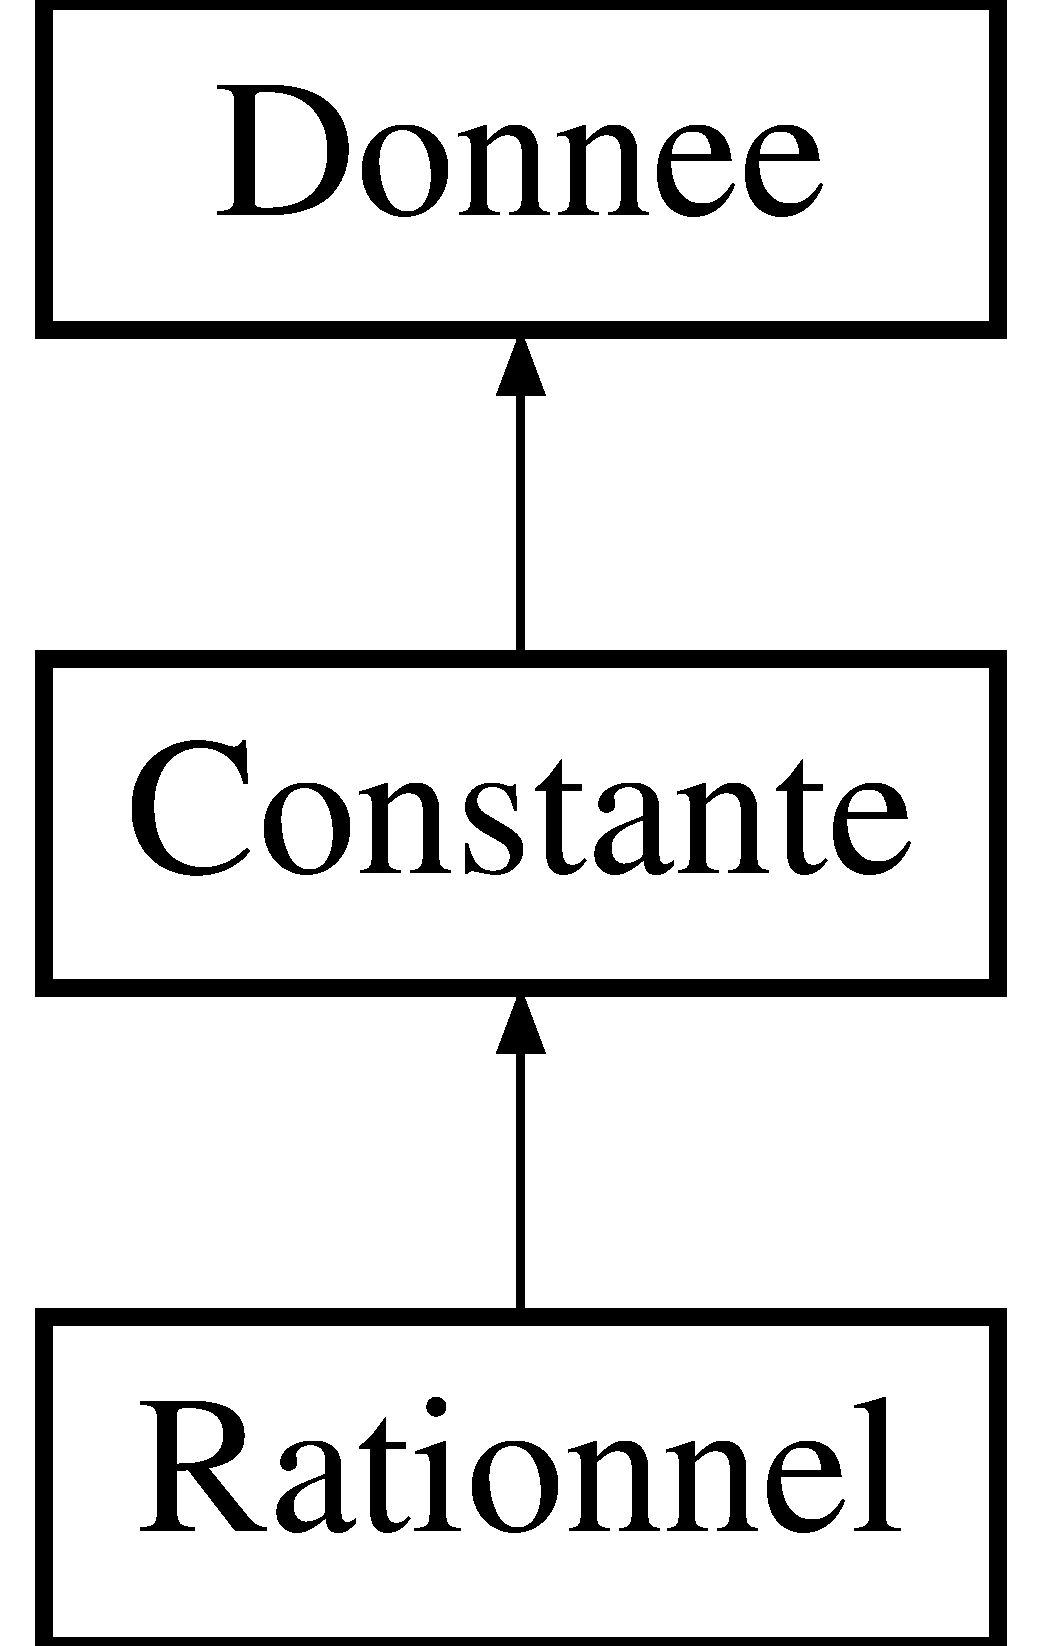
\includegraphics[height=3.000000cm]{class_rationnel}
\end{center}
\end{figure}
\subsection*{Public Member Functions}
\begin{DoxyCompactItemize}
\item 
\hyperlink{class_rationnel_ab7c6a6474b910a9b70e177299ef82baa}{Rationnel} (int a\-Int1=0, int a\-Int2=1)
\begin{DoxyCompactList}\small\item\em Constructeur de rationnel � partir de 2 constantes. \end{DoxyCompactList}\item 
\hyperlink{class_rationnel_a26a99758636a64b724fd6cf483695937}{Rationnel} (const Q\-String \&s)
\begin{DoxyCompactList}\small\item\em Constructeur de rationnel � partir d'une Q\-String. \end{DoxyCompactList}\item 
\hyperlink{class_rationnel_ad82fad96095d0a1303c42bf8fb7dc78f}{Rationnel} (const \hyperlink{class_rationnel}{Rationnel} $\ast$a\-Rationnel)
\begin{DoxyCompactList}\small\item\em Constructeur de recopie. \end{DoxyCompactList}\item 
\hyperlink{class_rationnel_aa5c9000f9f895d56c61677819075f0df}{Rationnel} (const \hyperlink{class_entier}{Entier} $\ast$a\-Entier)
\begin{DoxyCompactList}\small\item\em Constructeur de rationnel � partir d'entier. \end{DoxyCompactList}\item 
\hyperlink{class_rationnel_a394538bfd8a92370e327aa29ff614c5f}{Rationnel} (const \hyperlink{class_reel}{Reel} $\ast$a\-Reel)
\begin{DoxyCompactList}\small\item\em Constructeur de rationnel � partir d'entier. \end{DoxyCompactList}\item 
\hyperlink{class_rationnel_ab6abfabdca69244452c910a60cf4d1ff}{Rationnel} (const \hyperlink{class_complexe}{Complexe} $\ast$a\-Complexe)
\begin{DoxyCompactList}\small\item\em Constructeur de rationnel � partir d'entier. \end{DoxyCompactList}\item 
Q\-String \hyperlink{class_rationnel_a9a07315a6ccda0ff220ddebf6e650c2e}{to\-Q\-String} () const 
\begin{DoxyCompactList}\small\item\em M�thode permettant d'obtenir l'objet sous la forme d'une Qstring. \end{DoxyCompactList}\item 
\hyperlink{class_rationnel}{Rationnel} $\ast$ \hyperlink{class_rationnel_a32478893e33c8a1b7ada199592130eb6}{sign} ()
\begin{DoxyCompactList}\small\item\em Retourne un \hyperlink{class_rationnel}{Rationnel} ayant les meme valeur mais avec le sign invers� \end{DoxyCompactList}\item 
int \hyperlink{class_rationnel_ac9596f5d24cef6120c0cabcd7923aa29}{get\-Num} () const 
\begin{DoxyCompactList}\small\item\em Acccesseur au num�rateur. \end{DoxyCompactList}\item 
int \hyperlink{class_rationnel_a3809b3a6ac86e4b0a87bbf49f03dac6c}{get\-Denom} () const 
\begin{DoxyCompactList}\small\item\em Acccesseur au d�nominateur. \end{DoxyCompactList}\item 
void \hyperlink{class_rationnel_a84693706f85612a94811984b26f43b5e}{set\-Num} (int a\-Num)
\begin{DoxyCompactList}\small\item\em Modificateur du num�rateur. \end{DoxyCompactList}\item 
void \hyperlink{class_rationnel_ada2605f9e377cb574ba9ce83dbccf3c0}{set\-Denom} (int adenom)
\begin{DoxyCompactList}\small\item\em Modificateur du d�nominateur. \end{DoxyCompactList}\item 
int \hyperlink{class_rationnel_aced52c94493f4ec44492e3c8dcc07632}{pgcd} (int a, int b) const 
\begin{DoxyCompactList}\small\item\em Calcul du pgcd entre 2 nombre. \end{DoxyCompactList}\item 
void \hyperlink{class_rationnel_a12ee060e5fca5f4291b222983d727268}{simplifier} ()
\begin{DoxyCompactList}\small\item\em simplifie this pour que num et denum soit premier entre eux. \end{DoxyCompactList}\item 
\hyperlink{class_donnee}{Donnee} $\ast$ \hyperlink{class_rationnel_a59aa5ca6395412169b6eeea5ebed7d34}{operator+} (\hyperlink{class_donnee}{Donnee} $\ast$t)
\begin{DoxyCompactList}\small\item\em Operateur +. \end{DoxyCompactList}\item 
\hyperlink{class_donnee}{Donnee} $\ast$ \hyperlink{class_rationnel_a361a11f3a3f1a6a18a047e90f36da098}{operator/} (\hyperlink{class_donnee}{Donnee} $\ast$t)
\begin{DoxyCompactList}\small\item\em Operateur /. \end{DoxyCompactList}\item 
\hyperlink{class_donnee}{Donnee} $\ast$ \hyperlink{class_rationnel_a74b9d6827f9871aef113cc6eb665e1c8}{operator$\ast$} (\hyperlink{class_donnee}{Donnee} $\ast$t)
\begin{DoxyCompactList}\small\item\em Operateur $\ast$. \end{DoxyCompactList}\item 
\hyperlink{class_donnee}{Donnee} $\ast$ \hyperlink{class_rationnel_a939fb751ab75cc266ae5db7318ede036}{operator-\/} (\hyperlink{class_donnee}{Donnee} $\ast$t)
\begin{DoxyCompactList}\small\item\em Operateur -\/. \end{DoxyCompactList}\item 
\hyperlink{class_donnee}{Donnee} $\ast$ \hyperlink{class_rationnel_a4d56f2f93a4243db020e43d3be842da0}{puissance} (\hyperlink{class_donnee}{Donnee} $\ast$t)
\begin{DoxyCompactList}\small\item\em puissance \end{DoxyCompactList}\item 
\hyperlink{class_donnee}{Donnee} $\ast$ \hyperlink{class_rationnel_a5e60a48c0ec51f7c9ceef85c4feb1799}{mod} (\hyperlink{class_donnee}{Donnee} $\ast$t)
\begin{DoxyCompactList}\small\item\em mod \end{DoxyCompactList}\item 
\hyperlink{class_donnee}{Donnee} $\ast$ \hyperlink{class_rationnel_a5684344a9fb59a529c26e2003dddca2a}{my\-Sin} (int type\-Angle)
\begin{DoxyCompactList}\small\item\em my\-Sin \end{DoxyCompactList}\item 
\hyperlink{class_donnee}{Donnee} $\ast$ \hyperlink{class_rationnel_a995e0aa451d09c98fae7a5aa75fa2047}{my\-Cos} (int type\-Angle)
\begin{DoxyCompactList}\small\item\em my\-Cos \end{DoxyCompactList}\item 
\hyperlink{class_donnee}{Donnee} $\ast$ \hyperlink{class_rationnel_a973973c46875e00d8126ae06f637f7e9}{my\-Tan} (int type\-Angle)
\begin{DoxyCompactList}\small\item\em my\-Tan \end{DoxyCompactList}\item 
\hyperlink{class_donnee}{Donnee} $\ast$ \hyperlink{class_rationnel_ae89d62d68819b71ea51d01f8be3983c3}{my\-Sinh} (int type\-Angle)
\begin{DoxyCompactList}\small\item\em my\-Sinh \end{DoxyCompactList}\item 
\hyperlink{class_donnee}{Donnee} $\ast$ \hyperlink{class_rationnel_a20893c5f74c24222a5f80579b2aa2b2f}{my\-Cosh} (int type\-Angle)
\begin{DoxyCompactList}\small\item\em my\-Cosh \end{DoxyCompactList}\item 
\hyperlink{class_donnee}{Donnee} $\ast$ \hyperlink{class_rationnel_a5aedb2c197cda490f2dfe59eea937eb0}{my\-Tanh} (int type\-Angle)
\begin{DoxyCompactList}\small\item\em my\-Tanh \end{DoxyCompactList}\item 
\hyperlink{class_donnee}{Donnee} $\ast$ \hyperlink{class_rationnel_aa290c50b2917771b26a761e07c62a574}{my\-Ln} ()
\begin{DoxyCompactList}\small\item\em my\-Ln \end{DoxyCompactList}\item 
\hyperlink{class_donnee}{Donnee} $\ast$ \hyperlink{class_rationnel_aa3d968de9d5467e20681f802fdb20cc3}{my\-Log} ()
\begin{DoxyCompactList}\small\item\em my\-Log \end{DoxyCompactList}\item 
\hyperlink{class_donnee}{Donnee} $\ast$ \hyperlink{class_rationnel_ae860fd09ed94a2d60a197030822ada92}{my\-Inv} ()
\begin{DoxyCompactList}\small\item\em my\-Inv \end{DoxyCompactList}\item 
\hyperlink{class_donnee}{Donnee} $\ast$ \hyperlink{class_rationnel_a0305394c891df6b266852e22ab8dcca4}{my\-Sqrt} ()
\begin{DoxyCompactList}\small\item\em my\-Sqrt \end{DoxyCompactList}\item 
\hyperlink{class_donnee}{Donnee} $\ast$ \hyperlink{class_rationnel_add9f83270c7989dd0e984a3617337f8d}{my\-Sqr} ()
\begin{DoxyCompactList}\small\item\em my\-Sqr \end{DoxyCompactList}\item 
\hyperlink{class_donnee}{Donnee} $\ast$ \hyperlink{class_rationnel_a1bd3ee26d57c50c6eea7b62e671f3697}{my\-Cube} ()
\begin{DoxyCompactList}\small\item\em my\-Cube \end{DoxyCompactList}\item 
\hyperlink{class_donnee}{Donnee} $\ast$ \hyperlink{class_rationnel_aff2c6401047b78474705e1d392195bae}{my\-Fact} ()
\begin{DoxyCompactList}\small\item\em my\-Fact \end{DoxyCompactList}\item 
bool \hyperlink{class_rationnel_a61b12cda29f28591138415085bdc1a3d}{is\-Zero} ()
\begin{DoxyCompactList}\small\item\em is\-Zero \end{DoxyCompactList}\item 
bool \hyperlink{class_rationnel_a2180b4f282661ab844fee297be89018a}{is\-Neg} ()
\begin{DoxyCompactList}\small\item\em is\-Neg \end{DoxyCompactList}\end{DoxyCompactItemize}


\subsection{Detailed Description}
Classe des rationnels h�ritant de \hyperlink{class_constante}{Constante}. 

Pour fonctionner cette classe encapsule deux entiers (num�rateur et d�nominateur). Tout les op�rateurs sont �galements red�finis. 

\subsection{Constructor \& Destructor Documentation}
\hypertarget{class_rationnel_ab7c6a6474b910a9b70e177299ef82baa}{\index{Rationnel@{Rationnel}!Rationnel@{Rationnel}}
\index{Rationnel@{Rationnel}!Rationnel@{Rationnel}}
\subsubsection[{Rationnel}]{\setlength{\rightskip}{0pt plus 5cm}Rationnel\-::\-Rationnel (
\begin{DoxyParamCaption}
\item[{int}]{a\-Int1 = {\ttfamily 0}, }
\item[{int}]{a\-Int2 = {\ttfamily 1}}
\end{DoxyParamCaption}
)\hspace{0.3cm}{\ttfamily [inline]}}}\label{class_rationnel_ab7c6a6474b910a9b70e177299ef82baa}


Constructeur de rationnel � partir de 2 constantes. 

Les deux param�tres sont �valu�s pour pouvoir obtenir un entier.


\begin{DoxyParams}{Parameters}
{\em a\-Int1} & Premier param�tre = num�rateur \\
\hline
{\em a\-Int2} & deuxi�me param�tre = d�nominateur. \\
\hline
\end{DoxyParams}
\begin{DoxyReturn}{Returns}
Elle retourne le rationnel construit. 
\end{DoxyReturn}
\hypertarget{class_rationnel_a26a99758636a64b724fd6cf483695937}{\index{Rationnel@{Rationnel}!Rationnel@{Rationnel}}
\index{Rationnel@{Rationnel}!Rationnel@{Rationnel}}
\subsubsection[{Rationnel}]{\setlength{\rightskip}{0pt plus 5cm}Rationnel\-::\-Rationnel (
\begin{DoxyParamCaption}
\item[{const Q\-String \&}]{s}
\end{DoxyParamCaption}
)}}\label{class_rationnel_a26a99758636a64b724fd6cf483695937}


Constructeur de rationnel � partir d'une Q\-String. 

Le Q\-String est split� au niveau du / puis les valeurs s�par� donne le num�rateur et le d�nominateur.


\begin{DoxyParams}{Parameters}
{\em s} & Une Qstring de la forme '\textbackslash{}d+/\textbackslash{}d+' \\
\hline
\end{DoxyParams}
\begin{DoxyReturn}{Returns}
Elle retourne le rationnel construit. 
\end{DoxyReturn}
\hypertarget{class_rationnel_ad82fad96095d0a1303c42bf8fb7dc78f}{\index{Rationnel@{Rationnel}!Rationnel@{Rationnel}}
\index{Rationnel@{Rationnel}!Rationnel@{Rationnel}}
\subsubsection[{Rationnel}]{\setlength{\rightskip}{0pt plus 5cm}Rationnel\-::\-Rationnel (
\begin{DoxyParamCaption}
\item[{const {\bf Rationnel} $\ast$}]{a\-Rationnel}
\end{DoxyParamCaption}
)\hspace{0.3cm}{\ttfamily [inline]}}}\label{class_rationnel_ad82fad96095d0a1303c42bf8fb7dc78f}


Constructeur de recopie. 


\begin{DoxyParams}{Parameters}
{\em a\-Rationnel} & Un pointeur vers un autre rationnel \\
\hline
\end{DoxyParams}
\begin{DoxyReturn}{Returns}
Elle retourne le rationnel construit. 
\end{DoxyReturn}
\hypertarget{class_rationnel_aa5c9000f9f895d56c61677819075f0df}{\index{Rationnel@{Rationnel}!Rationnel@{Rationnel}}
\index{Rationnel@{Rationnel}!Rationnel@{Rationnel}}
\subsubsection[{Rationnel}]{\setlength{\rightskip}{0pt plus 5cm}Rationnel\-::\-Rationnel (
\begin{DoxyParamCaption}
\item[{const {\bf Entier} $\ast$}]{a\-Entier}
\end{DoxyParamCaption}
)}}\label{class_rationnel_aa5c9000f9f895d56c61677819075f0df}


Constructeur de rationnel � partir d'entier. 

Le rationnel construit aura la forme a\-Entier/1


\begin{DoxyParams}{Parameters}
{\em a\-Entier} & Un entier \\
\hline
\end{DoxyParams}
\begin{DoxyReturn}{Returns}
Elle retourne le rationnel construit. 
\end{DoxyReturn}
\hypertarget{class_rationnel_a394538bfd8a92370e327aa29ff614c5f}{\index{Rationnel@{Rationnel}!Rationnel@{Rationnel}}
\index{Rationnel@{Rationnel}!Rationnel@{Rationnel}}
\subsubsection[{Rationnel}]{\setlength{\rightskip}{0pt plus 5cm}Rationnel\-::\-Rationnel (
\begin{DoxyParamCaption}
\item[{const {\bf Reel} $\ast$}]{a\-Reel}
\end{DoxyParamCaption}
)}}\label{class_rationnel_a394538bfd8a92370e327aa29ff614c5f}


Constructeur de rationnel � partir d'entier. 

Le rationnel construit aura la forme a\-Reel/1


\begin{DoxyParams}{Parameters}
{\em a\-Reel} & Un reel \\
\hline
\end{DoxyParams}
\begin{DoxyReturn}{Returns}
Elle retourne le rationnel construit. 
\end{DoxyReturn}
\hypertarget{class_rationnel_ab6abfabdca69244452c910a60cf4d1ff}{\index{Rationnel@{Rationnel}!Rationnel@{Rationnel}}
\index{Rationnel@{Rationnel}!Rationnel@{Rationnel}}
\subsubsection[{Rationnel}]{\setlength{\rightskip}{0pt plus 5cm}Rationnel\-::\-Rationnel (
\begin{DoxyParamCaption}
\item[{const {\bf Complexe} $\ast$}]{a\-Complexe}
\end{DoxyParamCaption}
)}}\label{class_rationnel_ab6abfabdca69244452c910a60cf4d1ff}


Constructeur de rationnel � partir d'entier. 

Le rationnel construit aura la forme a\-Complexe/1


\begin{DoxyParams}{Parameters}
{\em a\-Complexe} & Un complexe \\
\hline
\end{DoxyParams}
\begin{DoxyReturn}{Returns}
Elle retourne le rationnel construit. 
\end{DoxyReturn}


\subsection{Member Function Documentation}
\hypertarget{class_rationnel_a3809b3a6ac86e4b0a87bbf49f03dac6c}{\index{Rationnel@{Rationnel}!get\-Denom@{get\-Denom}}
\index{get\-Denom@{get\-Denom}!Rationnel@{Rationnel}}
\subsubsection[{get\-Denom}]{\setlength{\rightskip}{0pt plus 5cm}int Rationnel\-::get\-Denom (
\begin{DoxyParamCaption}
{}
\end{DoxyParamCaption}
) const\hspace{0.3cm}{\ttfamily [inline]}}}\label{class_rationnel_a3809b3a6ac86e4b0a87bbf49f03dac6c}


Acccesseur au d�nominateur. 

\begin{DoxyReturn}{Returns}
Elle retourne le d�nominateur du rationnel 
\end{DoxyReturn}
\hypertarget{class_rationnel_ac9596f5d24cef6120c0cabcd7923aa29}{\index{Rationnel@{Rationnel}!get\-Num@{get\-Num}}
\index{get\-Num@{get\-Num}!Rationnel@{Rationnel}}
\subsubsection[{get\-Num}]{\setlength{\rightskip}{0pt plus 5cm}int Rationnel\-::get\-Num (
\begin{DoxyParamCaption}
{}
\end{DoxyParamCaption}
) const\hspace{0.3cm}{\ttfamily [inline]}}}\label{class_rationnel_ac9596f5d24cef6120c0cabcd7923aa29}


Acccesseur au num�rateur. 

\begin{DoxyReturn}{Returns}
Elle retourne le num�rateu du rationnel 
\end{DoxyReturn}
\hypertarget{class_rationnel_a2180b4f282661ab844fee297be89018a}{\index{Rationnel@{Rationnel}!is\-Neg@{is\-Neg}}
\index{is\-Neg@{is\-Neg}!Rationnel@{Rationnel}}
\subsubsection[{is\-Neg}]{\setlength{\rightskip}{0pt plus 5cm}bool Rationnel\-::is\-Neg (
\begin{DoxyParamCaption}
{}
\end{DoxyParamCaption}
)\hspace{0.3cm}{\ttfamily [inline]}, {\ttfamily [virtual]}}}\label{class_rationnel_a2180b4f282661ab844fee297be89018a}


is\-Neg 

Mathode permettant de savoir si la \hyperlink{class_donnee}{Donnee} est inferieure ou egale � 0 \begin{DoxyReturn}{Returns}
bool true si la \hyperlink{class_donnee}{Donnee} est inferieur ou egale � 0 
\end{DoxyReturn}


Implements \hyperlink{class_donnee_a0efb324f0c2e0682b971c3692c46e7c3}{Donnee}.

\hypertarget{class_rationnel_a61b12cda29f28591138415085bdc1a3d}{\index{Rationnel@{Rationnel}!is\-Zero@{is\-Zero}}
\index{is\-Zero@{is\-Zero}!Rationnel@{Rationnel}}
\subsubsection[{is\-Zero}]{\setlength{\rightskip}{0pt plus 5cm}bool Rationnel\-::is\-Zero (
\begin{DoxyParamCaption}
{}
\end{DoxyParamCaption}
)\hspace{0.3cm}{\ttfamily [inline]}, {\ttfamily [virtual]}}}\label{class_rationnel_a61b12cda29f28591138415085bdc1a3d}


is\-Zero 

Mathode permettant de savoir si la \hyperlink{class_donnee}{Donnee} est egale � 0 \begin{DoxyReturn}{Returns}
bool true si la \hyperlink{class_donnee}{Donnee} est egale � 0 
\end{DoxyReturn}


Implements \hyperlink{class_donnee_aad251e4148c791719d7d7bff18680611}{Donnee}.

\hypertarget{class_rationnel_a5e60a48c0ec51f7c9ceef85c4feb1799}{\index{Rationnel@{Rationnel}!mod@{mod}}
\index{mod@{mod}!Rationnel@{Rationnel}}
\subsubsection[{mod}]{\setlength{\rightskip}{0pt plus 5cm}{\bf Donnee}$\ast$ Rationnel\-::mod (
\begin{DoxyParamCaption}
\item[{{\bf Donnee} $\ast$}]{t}
\end{DoxyParamCaption}
)\hspace{0.3cm}{\ttfamily [inline]}, {\ttfamily [virtual]}}}\label{class_rationnel_a5e60a48c0ec51f7c9ceef85c4feb1799}


mod 

Implementation de l'op�rateur binaire modulo (methode virtuelle dans la classe mere) 
\begin{DoxyParams}{Parameters}
{\em t} & \-: Pointeur sur une donnee \\
\hline
\end{DoxyParams}
\begin{DoxyReturn}{Returns}
Pointeur sur donnee, resultat de l'operation 
\end{DoxyReturn}


Implements \hyperlink{class_donnee_a52ce1aa17ce2c613e98428f82e3f85b8}{Donnee}.

\hypertarget{class_rationnel_a995e0aa451d09c98fae7a5aa75fa2047}{\index{Rationnel@{Rationnel}!my\-Cos@{my\-Cos}}
\index{my\-Cos@{my\-Cos}!Rationnel@{Rationnel}}
\subsubsection[{my\-Cos}]{\setlength{\rightskip}{0pt plus 5cm}{\bf Donnee} $\ast$ Rationnel\-::my\-Cos (
\begin{DoxyParamCaption}
\item[{int}]{type\-Angle}
\end{DoxyParamCaption}
)\hspace{0.3cm}{\ttfamily [virtual]}}}\label{class_rationnel_a995e0aa451d09c98fae7a5aa75fa2047}


my\-Cos 

Implementation de l'op�rateur unaire cosinus (methode virtuelle dans la classe mere) 
\begin{DoxyParams}{Parameters}
{\em type\-Angle} & \-: entier, 0 si utilisation des degres, 1 si utilisation des radians \\
\hline
\end{DoxyParams}
\begin{DoxyReturn}{Returns}
Pointeur sur donnee, resultat de l'operation 
\end{DoxyReturn}


Implements \hyperlink{class_donnee_abd9a62bd6b7d189f50db350823e895c3}{Donnee}.

\hypertarget{class_rationnel_a20893c5f74c24222a5f80579b2aa2b2f}{\index{Rationnel@{Rationnel}!my\-Cosh@{my\-Cosh}}
\index{my\-Cosh@{my\-Cosh}!Rationnel@{Rationnel}}
\subsubsection[{my\-Cosh}]{\setlength{\rightskip}{0pt plus 5cm}{\bf Donnee} $\ast$ Rationnel\-::my\-Cosh (
\begin{DoxyParamCaption}
\item[{int}]{type\-Angle}
\end{DoxyParamCaption}
)\hspace{0.3cm}{\ttfamily [virtual]}}}\label{class_rationnel_a20893c5f74c24222a5f80579b2aa2b2f}


my\-Cosh 

Implementation de l'op�rateur unaire cosinush (methode virtuelle dans la classe mere) 
\begin{DoxyParams}{Parameters}
{\em type\-Angle} & \-: entier, 0 si utilisation des degres, 1 si utilisation des radians \\
\hline
\end{DoxyParams}
\begin{DoxyReturn}{Returns}
Pointeur sur donnee, resultat de l'operation 
\end{DoxyReturn}


Implements \hyperlink{class_donnee_afe9b3532677d394b4b596021b74b6d17}{Donnee}.

\hypertarget{class_rationnel_a1bd3ee26d57c50c6eea7b62e671f3697}{\index{Rationnel@{Rationnel}!my\-Cube@{my\-Cube}}
\index{my\-Cube@{my\-Cube}!Rationnel@{Rationnel}}
\subsubsection[{my\-Cube}]{\setlength{\rightskip}{0pt plus 5cm}{\bf Donnee} $\ast$ Rationnel\-::my\-Cube (
\begin{DoxyParamCaption}
{}
\end{DoxyParamCaption}
)\hspace{0.3cm}{\ttfamily [virtual]}}}\label{class_rationnel_a1bd3ee26d57c50c6eea7b62e671f3697}


my\-Cube 

Implementation de l'op�rateur unaire Cube (methode virtuelle dans la classe mere) \begin{DoxyReturn}{Returns}
Pointeur sur donnee, resultat de l'operation 
\end{DoxyReturn}


Implements \hyperlink{class_donnee_a875c21efdd22695c7999cfeb52ce4b2a}{Donnee}.

\hypertarget{class_rationnel_aff2c6401047b78474705e1d392195bae}{\index{Rationnel@{Rationnel}!my\-Fact@{my\-Fact}}
\index{my\-Fact@{my\-Fact}!Rationnel@{Rationnel}}
\subsubsection[{my\-Fact}]{\setlength{\rightskip}{0pt plus 5cm}{\bf Donnee}$\ast$ Rationnel\-::my\-Fact (
\begin{DoxyParamCaption}
{}
\end{DoxyParamCaption}
)\hspace{0.3cm}{\ttfamily [inline]}, {\ttfamily [virtual]}}}\label{class_rationnel_aff2c6401047b78474705e1d392195bae}


my\-Fact 

Implementation de l'op�rateur unaire fact (methode virtuelle dans la classe mere) \begin{DoxyReturn}{Returns}
Pointeur sur donnee, resultat de l'operation 
\end{DoxyReturn}


Implements \hyperlink{class_donnee_a79a2a3f835e09d0ed1888800c595a715}{Donnee}.

\hypertarget{class_rationnel_ae860fd09ed94a2d60a197030822ada92}{\index{Rationnel@{Rationnel}!my\-Inv@{my\-Inv}}
\index{my\-Inv@{my\-Inv}!Rationnel@{Rationnel}}
\subsubsection[{my\-Inv}]{\setlength{\rightskip}{0pt plus 5cm}{\bf Donnee} $\ast$ Rationnel\-::my\-Inv (
\begin{DoxyParamCaption}
{}
\end{DoxyParamCaption}
)\hspace{0.3cm}{\ttfamily [virtual]}}}\label{class_rationnel_ae860fd09ed94a2d60a197030822ada92}


my\-Inv 

Implementation de l'op�rateur unaire inv (methode virtuelle dans la classe mere) \begin{DoxyReturn}{Returns}
Pointeur sur donnee, resultat de l'operation 
\end{DoxyReturn}


Implements \hyperlink{class_donnee_ad84c463eb43d4b98bed081045160fea1}{Donnee}.

\hypertarget{class_rationnel_aa290c50b2917771b26a761e07c62a574}{\index{Rationnel@{Rationnel}!my\-Ln@{my\-Ln}}
\index{my\-Ln@{my\-Ln}!Rationnel@{Rationnel}}
\subsubsection[{my\-Ln}]{\setlength{\rightskip}{0pt plus 5cm}{\bf Donnee} $\ast$ Rationnel\-::my\-Ln (
\begin{DoxyParamCaption}
{}
\end{DoxyParamCaption}
)\hspace{0.3cm}{\ttfamily [virtual]}}}\label{class_rationnel_aa290c50b2917771b26a761e07c62a574}


my\-Ln 

Implementation de l'op�rateur unaire ln (methode virtuelle dans la classe mere) \begin{DoxyReturn}{Returns}
Pointeur sur donnee, resultat de l'operation 
\end{DoxyReturn}


Implements \hyperlink{class_donnee_ac24ba41baf90eb99bcf91145c541780a}{Donnee}.

\hypertarget{class_rationnel_aa3d968de9d5467e20681f802fdb20cc3}{\index{Rationnel@{Rationnel}!my\-Log@{my\-Log}}
\index{my\-Log@{my\-Log}!Rationnel@{Rationnel}}
\subsubsection[{my\-Log}]{\setlength{\rightskip}{0pt plus 5cm}{\bf Donnee} $\ast$ Rationnel\-::my\-Log (
\begin{DoxyParamCaption}
{}
\end{DoxyParamCaption}
)\hspace{0.3cm}{\ttfamily [virtual]}}}\label{class_rationnel_aa3d968de9d5467e20681f802fdb20cc3}


my\-Log 

Implementation de l'op�rateur unaire log (methode virtuelle dans la classe mere) \begin{DoxyReturn}{Returns}
Pointeur sur donnee, resultat de l'operation 
\end{DoxyReturn}


Implements \hyperlink{class_donnee_a7ac3f554be1fc579b02d9c877185cf50}{Donnee}.

\hypertarget{class_rationnel_a5684344a9fb59a529c26e2003dddca2a}{\index{Rationnel@{Rationnel}!my\-Sin@{my\-Sin}}
\index{my\-Sin@{my\-Sin}!Rationnel@{Rationnel}}
\subsubsection[{my\-Sin}]{\setlength{\rightskip}{0pt plus 5cm}{\bf Donnee} $\ast$ Rationnel\-::my\-Sin (
\begin{DoxyParamCaption}
\item[{int}]{type\-Angle}
\end{DoxyParamCaption}
)\hspace{0.3cm}{\ttfamily [virtual]}}}\label{class_rationnel_a5684344a9fb59a529c26e2003dddca2a}


my\-Sin 

Implementation de l'op�rateur unaire sinus (methode virtuelle dans la classe mere) 
\begin{DoxyParams}{Parameters}
{\em type\-Angle} & \-: entier, 0 si utilisation des degres, 1 si utilisation des radians \\
\hline
\end{DoxyParams}
\begin{DoxyReturn}{Returns}
Pointeur sur donnee, resultat de l'operation 
\end{DoxyReturn}


Implements \hyperlink{class_donnee_a86f71d87c3a69dc6dcede4b411d94043}{Donnee}.

\hypertarget{class_rationnel_ae89d62d68819b71ea51d01f8be3983c3}{\index{Rationnel@{Rationnel}!my\-Sinh@{my\-Sinh}}
\index{my\-Sinh@{my\-Sinh}!Rationnel@{Rationnel}}
\subsubsection[{my\-Sinh}]{\setlength{\rightskip}{0pt plus 5cm}{\bf Donnee} $\ast$ Rationnel\-::my\-Sinh (
\begin{DoxyParamCaption}
\item[{int}]{type\-Angle}
\end{DoxyParamCaption}
)\hspace{0.3cm}{\ttfamily [virtual]}}}\label{class_rationnel_ae89d62d68819b71ea51d01f8be3983c3}


my\-Sinh 

Implementation de l'op�rateur unaire sinush (methode virtuelle dans la classe mere) 
\begin{DoxyParams}{Parameters}
{\em type\-Angle} & \-: entier, 0 si utilisation des degres, 1 si utilisation des radians \\
\hline
\end{DoxyParams}
\begin{DoxyReturn}{Returns}
Pointeur sur donnee, resultat de l'operation 
\end{DoxyReturn}


Implements \hyperlink{class_donnee_af3c408a3fda8f24ee70f34fd8688fe63}{Donnee}.

\hypertarget{class_rationnel_add9f83270c7989dd0e984a3617337f8d}{\index{Rationnel@{Rationnel}!my\-Sqr@{my\-Sqr}}
\index{my\-Sqr@{my\-Sqr}!Rationnel@{Rationnel}}
\subsubsection[{my\-Sqr}]{\setlength{\rightskip}{0pt plus 5cm}{\bf Donnee} $\ast$ Rationnel\-::my\-Sqr (
\begin{DoxyParamCaption}
{}
\end{DoxyParamCaption}
)\hspace{0.3cm}{\ttfamily [virtual]}}}\label{class_rationnel_add9f83270c7989dd0e984a3617337f8d}


my\-Sqr 

Implementation de l'op�rateur unaire sqr (methode virtuelle dans la classe mere) \begin{DoxyReturn}{Returns}
Pointeur sur donnee, resultat de l'operation 
\end{DoxyReturn}


Implements \hyperlink{class_donnee_a708281bf8ddb3f6c33a100b3db925901}{Donnee}.

\hypertarget{class_rationnel_a0305394c891df6b266852e22ab8dcca4}{\index{Rationnel@{Rationnel}!my\-Sqrt@{my\-Sqrt}}
\index{my\-Sqrt@{my\-Sqrt}!Rationnel@{Rationnel}}
\subsubsection[{my\-Sqrt}]{\setlength{\rightskip}{0pt plus 5cm}{\bf Donnee} $\ast$ Rationnel\-::my\-Sqrt (
\begin{DoxyParamCaption}
{}
\end{DoxyParamCaption}
)\hspace{0.3cm}{\ttfamily [virtual]}}}\label{class_rationnel_a0305394c891df6b266852e22ab8dcca4}


my\-Sqrt 

Implementation de l'op�rateur unaire sqrt (methode virtuelle dans la classe mere) \begin{DoxyReturn}{Returns}
Pointeur sur donnee, resultat de l'operation 
\end{DoxyReturn}


Implements \hyperlink{class_donnee_a07484cd79bc071fbfc48ace5bcd94e8f}{Donnee}.

\hypertarget{class_rationnel_a973973c46875e00d8126ae06f637f7e9}{\index{Rationnel@{Rationnel}!my\-Tan@{my\-Tan}}
\index{my\-Tan@{my\-Tan}!Rationnel@{Rationnel}}
\subsubsection[{my\-Tan}]{\setlength{\rightskip}{0pt plus 5cm}{\bf Donnee} $\ast$ Rationnel\-::my\-Tan (
\begin{DoxyParamCaption}
\item[{int}]{type\-Angle}
\end{DoxyParamCaption}
)\hspace{0.3cm}{\ttfamily [virtual]}}}\label{class_rationnel_a973973c46875e00d8126ae06f637f7e9}


my\-Tan 

Implementation de l'op�rateur unaire tangente (methode virtuelle dans la classe mere) 
\begin{DoxyParams}{Parameters}
{\em type\-Angle} & \-: entier, 0 si utilisation des degres, 1 si utilisation des radians \\
\hline
\end{DoxyParams}
\begin{DoxyReturn}{Returns}
Pointeur sur donnee, resultat de l'operation 
\end{DoxyReturn}


Implements \hyperlink{class_donnee_ad3b4b9d20c0693915d9c17b528bed4d8}{Donnee}.

\hypertarget{class_rationnel_a5aedb2c197cda490f2dfe59eea937eb0}{\index{Rationnel@{Rationnel}!my\-Tanh@{my\-Tanh}}
\index{my\-Tanh@{my\-Tanh}!Rationnel@{Rationnel}}
\subsubsection[{my\-Tanh}]{\setlength{\rightskip}{0pt plus 5cm}{\bf Donnee} $\ast$ Rationnel\-::my\-Tanh (
\begin{DoxyParamCaption}
\item[{int}]{type\-Angle}
\end{DoxyParamCaption}
)\hspace{0.3cm}{\ttfamily [virtual]}}}\label{class_rationnel_a5aedb2c197cda490f2dfe59eea937eb0}


my\-Tanh 

Implementation de l'op�rateur unaire tangenteh (methode virtuelle dans la classe mere) 
\begin{DoxyParams}{Parameters}
{\em type\-Angle} & \-: entier, 0 si utilisation des degres, 1 si utilisation des radians \\
\hline
\end{DoxyParams}
\begin{DoxyReturn}{Returns}
Pointeur sur donnee, resultat de l'operation 
\end{DoxyReturn}


Implements \hyperlink{class_donnee_a20a90ca79d91dc75ea01cc3842b0e6dd}{Donnee}.

\hypertarget{class_rationnel_a74b9d6827f9871aef113cc6eb665e1c8}{\index{Rationnel@{Rationnel}!operator$\ast$@{operator$\ast$}}
\index{operator$\ast$@{operator$\ast$}!Rationnel@{Rationnel}}
\subsubsection[{operator$\ast$}]{\setlength{\rightskip}{0pt plus 5cm}{\bf Donnee} $\ast$ Rationnel\-::operator$\ast$ (
\begin{DoxyParamCaption}
\item[{{\bf Donnee} $\ast$}]{t}
\end{DoxyParamCaption}
)\hspace{0.3cm}{\ttfamily [virtual]}}}\label{class_rationnel_a74b9d6827f9871aef113cc6eb665e1c8}


Operateur $\ast$. 

Implementation de l'op�rateur binaire $\ast$ (methode virtuelle dans la classe mere) 
\begin{DoxyParams}{Parameters}
{\em t} & \-: Pointeur sur un type \\
\hline
\end{DoxyParams}
\begin{DoxyReturn}{Returns}
Pointeur sur type, resultat de l'operation 
\end{DoxyReturn}


Implements \hyperlink{class_donnee_ae655c41f021de91a35d652a8519d4eb2}{Donnee}.

\hypertarget{class_rationnel_a59aa5ca6395412169b6eeea5ebed7d34}{\index{Rationnel@{Rationnel}!operator+@{operator+}}
\index{operator+@{operator+}!Rationnel@{Rationnel}}
\subsubsection[{operator+}]{\setlength{\rightskip}{0pt plus 5cm}{\bf Donnee} $\ast$ Rationnel\-::operator+ (
\begin{DoxyParamCaption}
\item[{{\bf Donnee} $\ast$}]{t}
\end{DoxyParamCaption}
)\hspace{0.3cm}{\ttfamily [virtual]}}}\label{class_rationnel_a59aa5ca6395412169b6eeea5ebed7d34}


Operateur +. 

Implementation de l'op�rateur binaire + (methode virtuelle dans la classe mere) 
\begin{DoxyParams}{Parameters}
{\em t} & \-: Pointeur sur un type \\
\hline
\end{DoxyParams}
\begin{DoxyReturn}{Returns}
Pointeur sur type, resultat de l'operation 
\end{DoxyReturn}


Implements \hyperlink{class_donnee_acda2976724adeef2233e7077953c1a9a}{Donnee}.

\hypertarget{class_rationnel_a939fb751ab75cc266ae5db7318ede036}{\index{Rationnel@{Rationnel}!operator-\/@{operator-\/}}
\index{operator-\/@{operator-\/}!Rationnel@{Rationnel}}
\subsubsection[{operator-\/}]{\setlength{\rightskip}{0pt plus 5cm}{\bf Donnee} $\ast$ Rationnel\-::operator-\/ (
\begin{DoxyParamCaption}
\item[{{\bf Donnee} $\ast$}]{t}
\end{DoxyParamCaption}
)\hspace{0.3cm}{\ttfamily [virtual]}}}\label{class_rationnel_a939fb751ab75cc266ae5db7318ede036}


Operateur -\/. 

Implementation de l'op�rateur binaire -\/ (methode virtuelle dans la classe mere) 
\begin{DoxyParams}{Parameters}
{\em t} & \-: Pointeur sur un type \\
\hline
\end{DoxyParams}
\begin{DoxyReturn}{Returns}
Pointeur sur type, resultat de l'operation 
\end{DoxyReturn}


Implements \hyperlink{class_donnee_a053ea4f3f00b6e0a73b4ea453adca1be}{Donnee}.

\hypertarget{class_rationnel_a361a11f3a3f1a6a18a047e90f36da098}{\index{Rationnel@{Rationnel}!operator/@{operator/}}
\index{operator/@{operator/}!Rationnel@{Rationnel}}
\subsubsection[{operator/}]{\setlength{\rightskip}{0pt plus 5cm}{\bf Donnee} $\ast$ Rationnel\-::operator/ (
\begin{DoxyParamCaption}
\item[{{\bf Donnee} $\ast$}]{t}
\end{DoxyParamCaption}
)\hspace{0.3cm}{\ttfamily [virtual]}}}\label{class_rationnel_a361a11f3a3f1a6a18a047e90f36da098}


Operateur /. 

Implementation de l'op�rateur binaire / (methode virtuelle dans la classe mere) 
\begin{DoxyParams}{Parameters}
{\em t} & \-: Pointeur sur un type \\
\hline
\end{DoxyParams}
\begin{DoxyReturn}{Returns}
Pointeur sur type, resultat de l'operation 
\end{DoxyReturn}


Implements \hyperlink{class_donnee_abc63ffa0d62612446435ff1eca34344b}{Donnee}.

\hypertarget{class_rationnel_aced52c94493f4ec44492e3c8dcc07632}{\index{Rationnel@{Rationnel}!pgcd@{pgcd}}
\index{pgcd@{pgcd}!Rationnel@{Rationnel}}
\subsubsection[{pgcd}]{\setlength{\rightskip}{0pt plus 5cm}int Rationnel\-::pgcd (
\begin{DoxyParamCaption}
\item[{int}]{a, }
\item[{int}]{b}
\end{DoxyParamCaption}
) const}}\label{class_rationnel_aced52c94493f4ec44492e3c8dcc07632}


Calcul du pgcd entre 2 nombre. 

M�thode utilis� pour simplifier une fraction


\begin{DoxyParams}{Parameters}
{\em a} & Le premier entier \\
\hline
{\em b} & Le deuxi�me entier \\
\hline
\end{DoxyParams}
\begin{DoxyReturn}{Returns}
Elle retourne le pgcd entre a et b 
\end{DoxyReturn}
\hypertarget{class_rationnel_a4d56f2f93a4243db020e43d3be842da0}{\index{Rationnel@{Rationnel}!puissance@{puissance}}
\index{puissance@{puissance}!Rationnel@{Rationnel}}
\subsubsection[{puissance}]{\setlength{\rightskip}{0pt plus 5cm}{\bf Donnee} $\ast$ Rationnel\-::puissance (
\begin{DoxyParamCaption}
\item[{{\bf Donnee} $\ast$}]{t}
\end{DoxyParamCaption}
)\hspace{0.3cm}{\ttfamily [virtual]}}}\label{class_rationnel_a4d56f2f93a4243db020e43d3be842da0}


puissance 

Implementation de l'op�rateur binaire puissance (methode virtuelle dans la classe mere) 
\begin{DoxyParams}{Parameters}
{\em t,\-:} & Pointeur sur une donnee \\
\hline
\end{DoxyParams}
\begin{DoxyReturn}{Returns}
Pointeur sur donnee, resultat de l'operation 
\end{DoxyReturn}


Implements \hyperlink{class_donnee_af25f76885c91b1a497023c9dd2231990}{Donnee}.

\hypertarget{class_rationnel_ada2605f9e377cb574ba9ce83dbccf3c0}{\index{Rationnel@{Rationnel}!set\-Denom@{set\-Denom}}
\index{set\-Denom@{set\-Denom}!Rationnel@{Rationnel}}
\subsubsection[{set\-Denom}]{\setlength{\rightskip}{0pt plus 5cm}void Rationnel\-::set\-Denom (
\begin{DoxyParamCaption}
\item[{int}]{adenom}
\end{DoxyParamCaption}
)\hspace{0.3cm}{\ttfamily [inline]}}}\label{class_rationnel_ada2605f9e377cb574ba9ce83dbccf3c0}


Modificateur du d�nominateur. 


\begin{DoxyParams}{Parameters}
{\em adenom} & Le nouveau d�nominateur du rationnel \\
\hline
\end{DoxyParams}
\hypertarget{class_rationnel_a84693706f85612a94811984b26f43b5e}{\index{Rationnel@{Rationnel}!set\-Num@{set\-Num}}
\index{set\-Num@{set\-Num}!Rationnel@{Rationnel}}
\subsubsection[{set\-Num}]{\setlength{\rightskip}{0pt plus 5cm}void Rationnel\-::set\-Num (
\begin{DoxyParamCaption}
\item[{int}]{a\-Num}
\end{DoxyParamCaption}
)\hspace{0.3cm}{\ttfamily [inline]}}}\label{class_rationnel_a84693706f85612a94811984b26f43b5e}


Modificateur du num�rateur. 


\begin{DoxyParams}{Parameters}
{\em a\-Num} & Le nouveau num�rateu du rationnel \\
\hline
\end{DoxyParams}
\hypertarget{class_rationnel_a32478893e33c8a1b7ada199592130eb6}{\index{Rationnel@{Rationnel}!sign@{sign}}
\index{sign@{sign}!Rationnel@{Rationnel}}
\subsubsection[{sign}]{\setlength{\rightskip}{0pt plus 5cm}{\bf Rationnel}$\ast$ Rationnel\-::sign (
\begin{DoxyParamCaption}
{}
\end{DoxyParamCaption}
)\hspace{0.3cm}{\ttfamily [inline]}, {\ttfamily [virtual]}}}\label{class_rationnel_a32478893e33c8a1b7ada199592130eb6}


Retourne un \hyperlink{class_rationnel}{Rationnel} ayant les meme valeur mais avec le sign invers� 

Pour fonctionner, elle utilise le constructeur Rationnel(\-Constante $\ast$,\-Constante $\ast$)

\begin{DoxyReturn}{Returns}
Elle retourne le rationnel construit (=-\/this). 
\end{DoxyReturn}


Implements \hyperlink{class_constante_a3d218a44f46136c5d69f04821f100953}{Constante}.

\hypertarget{class_rationnel_a12ee060e5fca5f4291b222983d727268}{\index{Rationnel@{Rationnel}!simplifier@{simplifier}}
\index{simplifier@{simplifier}!Rationnel@{Rationnel}}
\subsubsection[{simplifier}]{\setlength{\rightskip}{0pt plus 5cm}void Rationnel\-::simplifier (
\begin{DoxyParamCaption}
{}
\end{DoxyParamCaption}
)}}\label{class_rationnel_a12ee060e5fca5f4291b222983d727268}


simplifie this pour que num et denum soit premier entre eux. 

Cette m�thode utilise \hyperlink{class_rationnel_aced52c94493f4ec44492e3c8dcc07632}{pgcd()} pour d�terminer comment simplifier this \hypertarget{class_rationnel_a9a07315a6ccda0ff220ddebf6e650c2e}{\index{Rationnel@{Rationnel}!to\-Q\-String@{to\-Q\-String}}
\index{to\-Q\-String@{to\-Q\-String}!Rationnel@{Rationnel}}
\subsubsection[{to\-Q\-String}]{\setlength{\rightskip}{0pt plus 5cm}Q\-String Rationnel\-::to\-Q\-String (
\begin{DoxyParamCaption}
{}
\end{DoxyParamCaption}
) const\hspace{0.3cm}{\ttfamily [virtual]}}}\label{class_rationnel_a9a07315a6ccda0ff220ddebf6e650c2e}


M�thode permettant d'obtenir l'objet sous la forme d'une Qstring. 

\begin{DoxyReturn}{Returns}
Elle retourne un Qstring tel qu'un rationnel puisse etre construit � partir de �a. 
\end{DoxyReturn}


Implements \hyperlink{class_donnee_ad96590e462f8db33aefca28ba8e31e52}{Donnee}.



The documentation for this class was generated from the following files\-:\begin{DoxyCompactItemize}
\item 
\hyperlink{rationnel_8h}{rationnel.\-h}\item 
rationnel.\-cpp\end{DoxyCompactItemize}

\hypertarget{class_reel}{\section{Reel Class Reference}
\label{class_reel}\index{Reel@{Reel}}
}


Classe des reels h�ritant de \hyperlink{class_constante}{Constante}.  




{\ttfamily \#include $<$reel.\-h$>$}

Inheritance diagram for Reel\-:\begin{figure}[H]
\begin{center}
\leavevmode
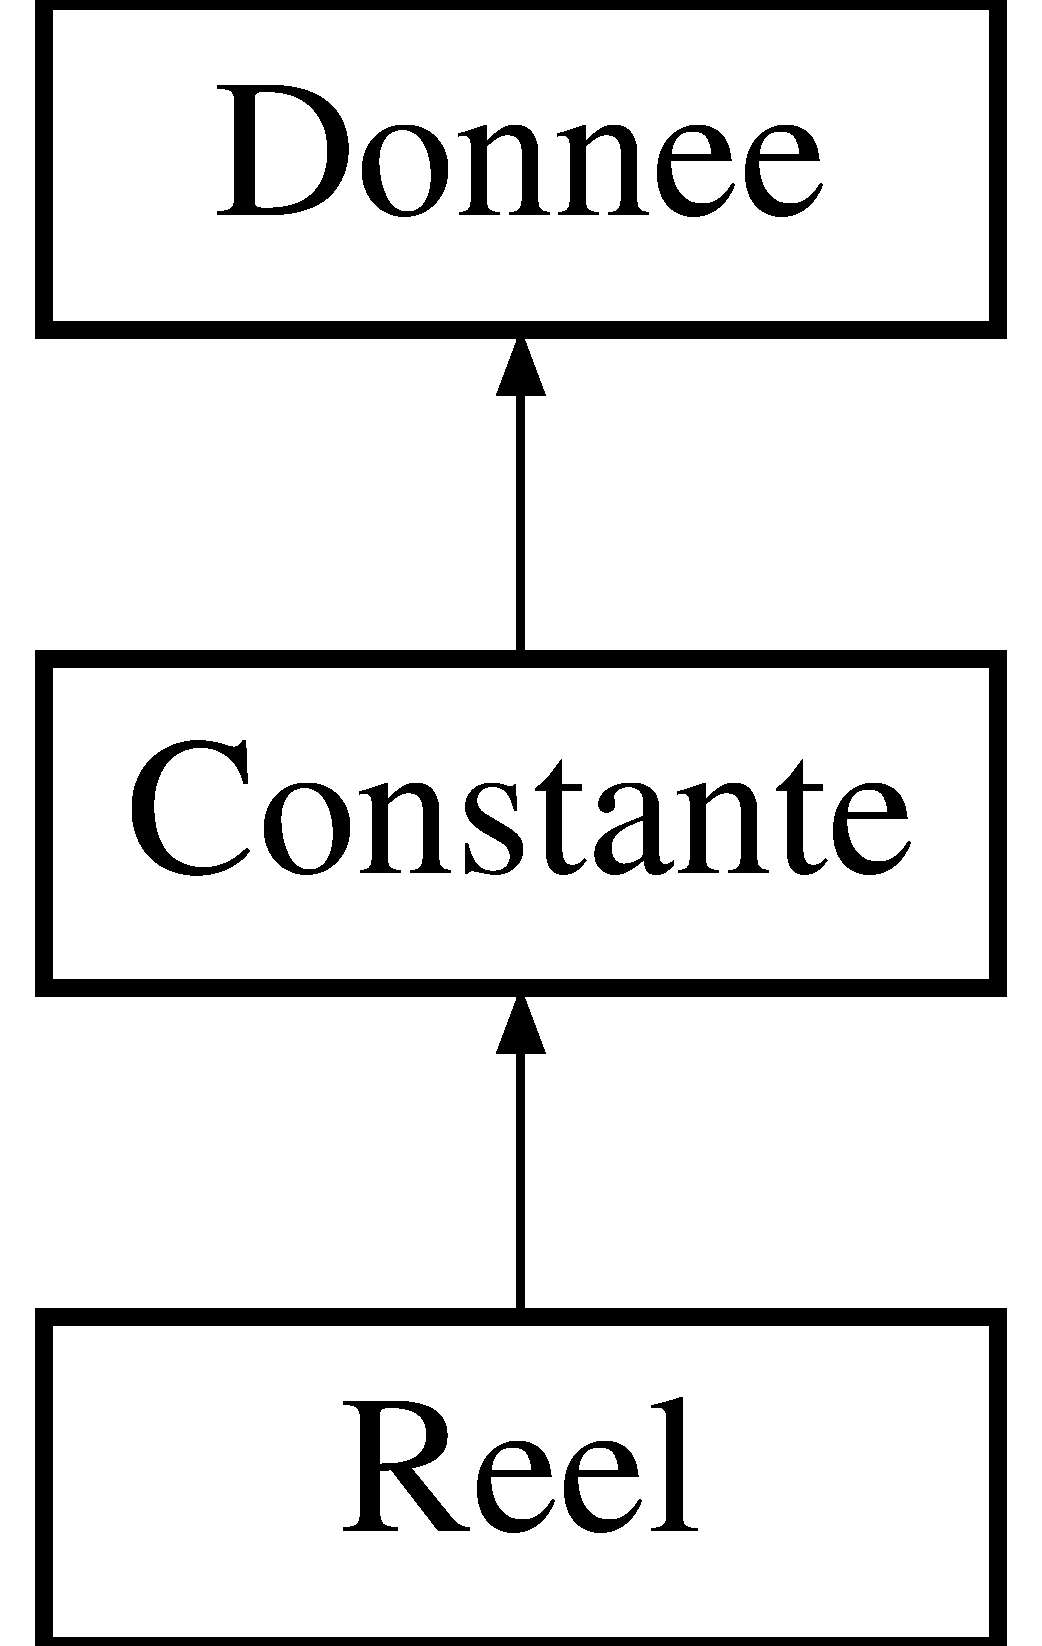
\includegraphics[height=3.000000cm]{class_reel}
\end{center}
\end{figure}
\subsection*{Public Member Functions}
\begin{DoxyCompactItemize}
\item 
\hyperlink{class_reel_a10756227cbba51f1b70ad8ec1ac42f8b}{Reel} (double val=0)
\begin{DoxyCompactList}\small\item\em Constructeur de reel � partir d'un double. \end{DoxyCompactList}\item 
\hyperlink{class_reel_af9105ec017abdcbd402256d5dd989538}{Reel} (const Q\-String \&a\-Q\-String=\char`\"{}0\char`\"{})
\begin{DoxyCompactList}\small\item\em Constructeur de reel � partir d'une Qstring. \end{DoxyCompactList}\item 
\hyperlink{class_reel_a6a2b775e7a796588702ddfab0aceb6bf}{Reel} (const \hyperlink{class_reel}{Reel} $\ast$a\-Reel)
\begin{DoxyCompactList}\small\item\em Constructeur de recopie d'un reel. \end{DoxyCompactList}\item 
\hyperlink{class_reel_ae70bb4263223a3791df2f531b845a015}{Reel} (const \hyperlink{class_entier}{Entier} $\ast$a\-Entier)
\begin{DoxyCompactList}\small\item\em Constructeur de reel � partir d'entier. \end{DoxyCompactList}\item 
\hyperlink{class_reel_a4f80c8d4d59730902c3e3d2e461cabc4}{Reel} (const \hyperlink{class_rationnel}{Rationnel} $\ast$a\-Rationnel)
\begin{DoxyCompactList}\small\item\em Constructeur de reel � partir d'un rationnel. \end{DoxyCompactList}\item 
\hyperlink{class_reel_a839d54e75df6556440b9af49fba5e78a}{Reel} (const \hyperlink{class_complexe}{Complexe} $\ast$a\-Complexe)
\begin{DoxyCompactList}\small\item\em Constructeur de reel � partir d'entier. \end{DoxyCompactList}\item 
virtual Q\-String \hyperlink{class_reel_a1da2b61268f280611649c19ca60b81a1}{to\-Q\-String} () const 
\begin{DoxyCompactList}\small\item\em M�thode permettant d'obtenir l'objet sous la forme d'une Qstring. \end{DoxyCompactList}\item 
double \hyperlink{class_reel_a6412ad4d84dcd302c1fae1f7ec3ede46}{get\-Valeur} () const 
\begin{DoxyCompactList}\small\item\em Accesseur � la valeur du reel. \end{DoxyCompactList}\item 
void \hyperlink{class_reel_af63b2f08328328914ebca127a9c84ca2}{set\-Valeur} (double a\-Valeur)
\begin{DoxyCompactList}\small\item\em Modificateur de la valeur du reel. \end{DoxyCompactList}\item 
int \hyperlink{class_reel_a4eff1ac5d600d369455c89d4361c8d9f}{get\-Taille} () const 
\begin{DoxyCompactList}\small\item\em Fonction permettant de calculer le nombre digit de this apr�s la virgule. \end{DoxyCompactList}\item 
\hyperlink{class_reel}{Reel} $\ast$ \hyperlink{class_reel_ae80b92f821de4ad1dc327ff7bdd5fc0e}{sign} ()
\begin{DoxyCompactList}\small\item\em Retourne un reel ayant les meme valeur mais avec le sign invers� \end{DoxyCompactList}\item 
\hyperlink{class_donnee}{Donnee} $\ast$ \hyperlink{class_reel_a3168acb7cf186497b81e3fca3478df14}{operator+} (\hyperlink{class_donnee}{Donnee} $\ast$t)
\begin{DoxyCompactList}\small\item\em Operateur +. \end{DoxyCompactList}\item 
\hyperlink{class_donnee}{Donnee} $\ast$ \hyperlink{class_reel_aa3da104c9f5f9e26fc33dcd642599623}{operator/} (\hyperlink{class_donnee}{Donnee} $\ast$t)
\begin{DoxyCompactList}\small\item\em Operateur /. \end{DoxyCompactList}\item 
\hyperlink{class_donnee}{Donnee} $\ast$ \hyperlink{class_reel_abe7e33c75910914c8297c08e94a64f7a}{operator$\ast$} (\hyperlink{class_donnee}{Donnee} $\ast$t)
\begin{DoxyCompactList}\small\item\em Operateur $\ast$. \end{DoxyCompactList}\item 
\hyperlink{class_donnee}{Donnee} $\ast$ \hyperlink{class_reel_ad0db0d6d4e512e538565fa308d6073fd}{operator-\/} (\hyperlink{class_donnee}{Donnee} $\ast$t)
\begin{DoxyCompactList}\small\item\em Operateur -\/. \end{DoxyCompactList}\item 
virtual \hyperlink{class_donnee}{Donnee} $\ast$ \hyperlink{class_reel_ad98206e433666510680a90ef49d68f84}{puissance} (\hyperlink{class_donnee}{Donnee} $\ast$t)
\begin{DoxyCompactList}\small\item\em puissance \end{DoxyCompactList}\item 
virtual \hyperlink{class_donnee}{Donnee} $\ast$ \hyperlink{class_reel_a04e3cd432ff3e82f9dab85951a018e9f}{mod} (\hyperlink{class_donnee}{Donnee} $\ast$t)
\begin{DoxyCompactList}\small\item\em mod \end{DoxyCompactList}\item 
virtual \hyperlink{class_donnee}{Donnee} $\ast$ \hyperlink{class_reel_ae484e067cb6405161a98152505ee9e06}{my\-Sin} (int type\-Angle)
\begin{DoxyCompactList}\small\item\em my\-Sin \end{DoxyCompactList}\item 
virtual \hyperlink{class_donnee}{Donnee} $\ast$ \hyperlink{class_reel_ace93d2421059d437af6f2ac319d91558}{my\-Cos} (int type\-Angle)
\begin{DoxyCompactList}\small\item\em my\-Cos \end{DoxyCompactList}\item 
virtual \hyperlink{class_donnee}{Donnee} $\ast$ \hyperlink{class_reel_a614dd1dd31c044eaf50551bc5089fa57}{my\-Tan} (int type\-Angle)
\begin{DoxyCompactList}\small\item\em my\-Tan \end{DoxyCompactList}\item 
virtual \hyperlink{class_donnee}{Donnee} $\ast$ \hyperlink{class_reel_a4f10a03b1ef5569df7a084bc2e9eb500}{my\-Sinh} (int type\-Angle)
\begin{DoxyCompactList}\small\item\em my\-Sinh \end{DoxyCompactList}\item 
virtual \hyperlink{class_donnee}{Donnee} $\ast$ \hyperlink{class_reel_abc4f6a7bbeeeb2d4646b014b10175222}{my\-Cosh} (int type\-Angle)
\begin{DoxyCompactList}\small\item\em my\-Cosh \end{DoxyCompactList}\item 
virtual \hyperlink{class_donnee}{Donnee} $\ast$ \hyperlink{class_reel_a8c9980059124e0feed84a90302c9351f}{my\-Tanh} (int type\-Angle)
\begin{DoxyCompactList}\small\item\em my\-Tanh \end{DoxyCompactList}\item 
virtual \hyperlink{class_donnee}{Donnee} $\ast$ \hyperlink{class_reel_a1b412487797f16aba98165997ce2851d}{my\-Ln} ()
\begin{DoxyCompactList}\small\item\em my\-Ln \end{DoxyCompactList}\item 
virtual \hyperlink{class_donnee}{Donnee} $\ast$ \hyperlink{class_reel_af9aad19f270974562a5a622bf9b3f554}{my\-Log} ()
\begin{DoxyCompactList}\small\item\em my\-Log \end{DoxyCompactList}\item 
virtual \hyperlink{class_donnee}{Donnee} $\ast$ \hyperlink{class_reel_af3e0e55294f6501a7a8d92d9174ed5f2}{my\-Inv} ()
\begin{DoxyCompactList}\small\item\em my\-Inv \end{DoxyCompactList}\item 
virtual \hyperlink{class_donnee}{Donnee} $\ast$ \hyperlink{class_reel_a3371cccfc481eec9f7b4aedbc5ca3789}{my\-Sqrt} ()
\begin{DoxyCompactList}\small\item\em my\-Sqrt \end{DoxyCompactList}\item 
virtual \hyperlink{class_donnee}{Donnee} $\ast$ \hyperlink{class_reel_a3ac200c65a8f74746c48d9245de890e1}{my\-Sqr} ()
\begin{DoxyCompactList}\small\item\em my\-Sqr \end{DoxyCompactList}\item 
virtual \hyperlink{class_donnee}{Donnee} $\ast$ \hyperlink{class_reel_aa716c8d1746da3630db9b6b1b18f3958}{my\-Cube} ()
\begin{DoxyCompactList}\small\item\em my\-Cube \end{DoxyCompactList}\item 
virtual \hyperlink{class_donnee}{Donnee} $\ast$ \hyperlink{class_reel_a2556b47a496658f8e046790450fd6881}{my\-Fact} ()
\begin{DoxyCompactList}\small\item\em my\-Fact \end{DoxyCompactList}\item 
bool \hyperlink{class_reel_a55940f0104fc9a8039bd102f1f88ba93}{is\-Zero} ()
\begin{DoxyCompactList}\small\item\em is\-Zero \end{DoxyCompactList}\item 
bool \hyperlink{class_reel_aac7382cedfb25716bb61f35f41839218}{is\-Neg} ()
\begin{DoxyCompactList}\small\item\em is\-Neg \end{DoxyCompactList}\end{DoxyCompactItemize}


\subsection{Detailed Description}
Classe des reels h�ritant de \hyperlink{class_constante}{Constante}. 

Pour fonctionner cette classe encapsule un double. Tout les op�rateurs sont �galement red�finis. 

\subsection{Constructor \& Destructor Documentation}
\hypertarget{class_reel_a10756227cbba51f1b70ad8ec1ac42f8b}{\index{Reel@{Reel}!Reel@{Reel}}
\index{Reel@{Reel}!Reel@{Reel}}
\subsubsection[{Reel}]{\setlength{\rightskip}{0pt plus 5cm}Reel\-::\-Reel (
\begin{DoxyParamCaption}
\item[{double}]{val = {\ttfamily 0}}
\end{DoxyParamCaption}
)\hspace{0.3cm}{\ttfamily [inline]}}}\label{class_reel_a10756227cbba51f1b70ad8ec1ac42f8b}


Constructeur de reel � partir d'un double. 


\begin{DoxyParams}{Parameters}
{\em val} & Valeur d'initialisation de la valeur de this \\
\hline
\end{DoxyParams}
\begin{DoxyReturn}{Returns}
Elle retourne le reel construit. 
\end{DoxyReturn}
\hypertarget{class_reel_af9105ec017abdcbd402256d5dd989538}{\index{Reel@{Reel}!Reel@{Reel}}
\index{Reel@{Reel}!Reel@{Reel}}
\subsubsection[{Reel}]{\setlength{\rightskip}{0pt plus 5cm}Reel\-::\-Reel (
\begin{DoxyParamCaption}
\item[{const Q\-String \&}]{a\-Q\-String = {\ttfamily \char`\"{}0\char`\"{}}}
\end{DoxyParamCaption}
)\hspace{0.3cm}{\ttfamily [inline]}}}\label{class_reel_af9105ec017abdcbd402256d5dd989538}


Constructeur de reel � partir d'une Qstring. 


\begin{DoxyParams}{Parameters}
{\em a\-Q\-String} & Il s'agit d'un Qstring de la forme '\textbackslash{}d+(($|$) \textbackslash{}d+)?) \\
\hline
\end{DoxyParams}
\begin{DoxyReturn}{Returns}
Elle retourne le reel construit. 
\end{DoxyReturn}
\hypertarget{class_reel_a6a2b775e7a796588702ddfab0aceb6bf}{\index{Reel@{Reel}!Reel@{Reel}}
\index{Reel@{Reel}!Reel@{Reel}}
\subsubsection[{Reel}]{\setlength{\rightskip}{0pt plus 5cm}Reel\-::\-Reel (
\begin{DoxyParamCaption}
\item[{const {\bf Reel} $\ast$}]{a\-Reel}
\end{DoxyParamCaption}
)\hspace{0.3cm}{\ttfamily [inline]}}}\label{class_reel_a6a2b775e7a796588702ddfab0aceb6bf}


Constructeur de recopie d'un reel. 


\begin{DoxyParams}{Parameters}
{\em a\-Reel} & Un pointeur vers un \hyperlink{class_reel}{Reel} \\
\hline
\end{DoxyParams}
\begin{DoxyReturn}{Returns}
Elle retourne le reel construit. 
\end{DoxyReturn}
\hypertarget{class_reel_ae70bb4263223a3791df2f531b845a015}{\index{Reel@{Reel}!Reel@{Reel}}
\index{Reel@{Reel}!Reel@{Reel}}
\subsubsection[{Reel}]{\setlength{\rightskip}{0pt plus 5cm}Reel\-::\-Reel (
\begin{DoxyParamCaption}
\item[{const {\bf Entier} $\ast$}]{a\-Entier}
\end{DoxyParamCaption}
)}}\label{class_reel_ae70bb4263223a3791df2f531b845a015}


Constructeur de reel � partir d'entier. 

Le reel construit aura la forme a\-Entier


\begin{DoxyParams}{Parameters}
{\em a\-Entier} & Un entier \\
\hline
\end{DoxyParams}
\begin{DoxyReturn}{Returns}
Elle retourne le reel construit. 
\end{DoxyReturn}
\hypertarget{class_reel_a4f80c8d4d59730902c3e3d2e461cabc4}{\index{Reel@{Reel}!Reel@{Reel}}
\index{Reel@{Reel}!Reel@{Reel}}
\subsubsection[{Reel}]{\setlength{\rightskip}{0pt plus 5cm}Reel\-::\-Reel (
\begin{DoxyParamCaption}
\item[{const {\bf Rationnel} $\ast$}]{a\-Rationnel}
\end{DoxyParamCaption}
)}}\label{class_reel_a4f80c8d4d59730902c3e3d2e461cabc4}


Constructeur de reel � partir d'un rationnel. 

Le reel construit aura la forme a\-Reel/1


\begin{DoxyParams}{Parameters}
{\em a\-Rationnel} & Un \hyperlink{class_rationnel}{Rationnel} \\
\hline
\end{DoxyParams}
\begin{DoxyReturn}{Returns}
Elle retourne le reel construit. 
\end{DoxyReturn}
\hypertarget{class_reel_a839d54e75df6556440b9af49fba5e78a}{\index{Reel@{Reel}!Reel@{Reel}}
\index{Reel@{Reel}!Reel@{Reel}}
\subsubsection[{Reel}]{\setlength{\rightskip}{0pt plus 5cm}Reel\-::\-Reel (
\begin{DoxyParamCaption}
\item[{const {\bf Complexe} $\ast$}]{a\-Complexe}
\end{DoxyParamCaption}
)}}\label{class_reel_a839d54e75df6556440b9af49fba5e78a}


Constructeur de reel � partir d'entier. 

Le reel construit aura la forme a\-Complexe-\/$>$get\-P\-Re()


\begin{DoxyParams}{Parameters}
{\em a\-Complexe} & Un complexe \\
\hline
\end{DoxyParams}
\begin{DoxyReturn}{Returns}
Elle retourne le reel construit. 
\end{DoxyReturn}


\subsection{Member Function Documentation}
\hypertarget{class_reel_a4eff1ac5d600d369455c89d4361c8d9f}{\index{Reel@{Reel}!get\-Taille@{get\-Taille}}
\index{get\-Taille@{get\-Taille}!Reel@{Reel}}
\subsubsection[{get\-Taille}]{\setlength{\rightskip}{0pt plus 5cm}int Reel\-::get\-Taille (
\begin{DoxyParamCaption}
{}
\end{DoxyParamCaption}
) const\hspace{0.3cm}{\ttfamily [inline]}}}\label{class_reel_a4eff1ac5d600d369455c89d4361c8d9f}


Fonction permettant de calculer le nombre digit de this apr�s la virgule. 

\begin{DoxyReturn}{Returns}
Elle retourne le nombre de de chiffre apr�s la virgule. 
\end{DoxyReturn}
\hypertarget{class_reel_a6412ad4d84dcd302c1fae1f7ec3ede46}{\index{Reel@{Reel}!get\-Valeur@{get\-Valeur}}
\index{get\-Valeur@{get\-Valeur}!Reel@{Reel}}
\subsubsection[{get\-Valeur}]{\setlength{\rightskip}{0pt plus 5cm}double Reel\-::get\-Valeur (
\begin{DoxyParamCaption}
{}
\end{DoxyParamCaption}
) const\hspace{0.3cm}{\ttfamily [inline]}}}\label{class_reel_a6412ad4d84dcd302c1fae1f7ec3ede46}


Accesseur � la valeur du reel. 

\begin{DoxyReturn}{Returns}
Elle retourne la valeur de l'objet 
\end{DoxyReturn}
\hypertarget{class_reel_aac7382cedfb25716bb61f35f41839218}{\index{Reel@{Reel}!is\-Neg@{is\-Neg}}
\index{is\-Neg@{is\-Neg}!Reel@{Reel}}
\subsubsection[{is\-Neg}]{\setlength{\rightskip}{0pt plus 5cm}bool Reel\-::is\-Neg (
\begin{DoxyParamCaption}
{}
\end{DoxyParamCaption}
)\hspace{0.3cm}{\ttfamily [inline]}, {\ttfamily [virtual]}}}\label{class_reel_aac7382cedfb25716bb61f35f41839218}


is\-Neg 

Mathode permettant de savoir si la \hyperlink{class_donnee}{Donnee} est inferieure ou egale � 0 \begin{DoxyReturn}{Returns}
bool true si la \hyperlink{class_donnee}{Donnee} est inferieur ou egale � 0 
\end{DoxyReturn}


Implements \hyperlink{class_donnee_a0efb324f0c2e0682b971c3692c46e7c3}{Donnee}.

\hypertarget{class_reel_a55940f0104fc9a8039bd102f1f88ba93}{\index{Reel@{Reel}!is\-Zero@{is\-Zero}}
\index{is\-Zero@{is\-Zero}!Reel@{Reel}}
\subsubsection[{is\-Zero}]{\setlength{\rightskip}{0pt plus 5cm}bool Reel\-::is\-Zero (
\begin{DoxyParamCaption}
{}
\end{DoxyParamCaption}
)\hspace{0.3cm}{\ttfamily [inline]}, {\ttfamily [virtual]}}}\label{class_reel_a55940f0104fc9a8039bd102f1f88ba93}


is\-Zero 

Mathode permettant de savoir si la \hyperlink{class_donnee}{Donnee} est egale � 0 \begin{DoxyReturn}{Returns}
bool true si la \hyperlink{class_donnee}{Donnee} est egale � 0 
\end{DoxyReturn}


Implements \hyperlink{class_donnee_aad251e4148c791719d7d7bff18680611}{Donnee}.

\hypertarget{class_reel_a04e3cd432ff3e82f9dab85951a018e9f}{\index{Reel@{Reel}!mod@{mod}}
\index{mod@{mod}!Reel@{Reel}}
\subsubsection[{mod}]{\setlength{\rightskip}{0pt plus 5cm}virtual {\bf Donnee}$\ast$ Reel\-::mod (
\begin{DoxyParamCaption}
\item[{{\bf Donnee} $\ast$}]{t}
\end{DoxyParamCaption}
)\hspace{0.3cm}{\ttfamily [inline]}, {\ttfamily [virtual]}}}\label{class_reel_a04e3cd432ff3e82f9dab85951a018e9f}


mod 

Implementation de l'op�rateur binaire modulo (methode virtuelle dans la classe mere) 
\begin{DoxyParams}{Parameters}
{\em t} & Donnee$\ast$\-: Pointeur sur une donnee \\
\hline
\end{DoxyParams}
\begin{DoxyReturn}{Returns}
Pointeur sur donnee, resultat de l'operation 
\end{DoxyReturn}


Implements \hyperlink{class_donnee_a52ce1aa17ce2c613e98428f82e3f85b8}{Donnee}.

\hypertarget{class_reel_ace93d2421059d437af6f2ac319d91558}{\index{Reel@{Reel}!my\-Cos@{my\-Cos}}
\index{my\-Cos@{my\-Cos}!Reel@{Reel}}
\subsubsection[{my\-Cos}]{\setlength{\rightskip}{0pt plus 5cm}{\bf Donnee} $\ast$ Reel\-::my\-Cos (
\begin{DoxyParamCaption}
\item[{int}]{type\-Angle}
\end{DoxyParamCaption}
)\hspace{0.3cm}{\ttfamily [virtual]}}}\label{class_reel_ace93d2421059d437af6f2ac319d91558}


my\-Cos 

Implementation de l'op�rateur unaire cosinus (methode virtuelle dans la classe mere) 
\begin{DoxyParams}{Parameters}
{\em type\-Angle} & \-: entier, 0 si utilisation des degres, 1 si utilisation des radians \\
\hline
\end{DoxyParams}
\begin{DoxyReturn}{Returns}
Pointeur sur donnee, resultat de l'operation 
\end{DoxyReturn}


Implements \hyperlink{class_donnee_abd9a62bd6b7d189f50db350823e895c3}{Donnee}.

\hypertarget{class_reel_abc4f6a7bbeeeb2d4646b014b10175222}{\index{Reel@{Reel}!my\-Cosh@{my\-Cosh}}
\index{my\-Cosh@{my\-Cosh}!Reel@{Reel}}
\subsubsection[{my\-Cosh}]{\setlength{\rightskip}{0pt plus 5cm}{\bf Donnee} $\ast$ Reel\-::my\-Cosh (
\begin{DoxyParamCaption}
\item[{int}]{type\-Angle}
\end{DoxyParamCaption}
)\hspace{0.3cm}{\ttfamily [virtual]}}}\label{class_reel_abc4f6a7bbeeeb2d4646b014b10175222}


my\-Cosh 

Implementation de l'op�rateur unaire cosinush (methode virtuelle dans la classe mere) 
\begin{DoxyParams}{Parameters}
{\em type\-Angle} & \-: entier, 0 si utilisation des degres, 1 si utilisation des radians \\
\hline
\end{DoxyParams}
\begin{DoxyReturn}{Returns}
Pointeur sur donnee, resultat de l'operation 
\end{DoxyReturn}


Implements \hyperlink{class_donnee_afe9b3532677d394b4b596021b74b6d17}{Donnee}.

\hypertarget{class_reel_aa716c8d1746da3630db9b6b1b18f3958}{\index{Reel@{Reel}!my\-Cube@{my\-Cube}}
\index{my\-Cube@{my\-Cube}!Reel@{Reel}}
\subsubsection[{my\-Cube}]{\setlength{\rightskip}{0pt plus 5cm}{\bf Donnee} $\ast$ Reel\-::my\-Cube (
\begin{DoxyParamCaption}
{}
\end{DoxyParamCaption}
)\hspace{0.3cm}{\ttfamily [virtual]}}}\label{class_reel_aa716c8d1746da3630db9b6b1b18f3958}


my\-Cube 

Implementation de l'op�rateur unaire Cube (methode virtuelle dans la classe mere) \begin{DoxyReturn}{Returns}
Pointeur sur donnee, resultat de l'operation 
\end{DoxyReturn}


Implements \hyperlink{class_donnee_a875c21efdd22695c7999cfeb52ce4b2a}{Donnee}.

\hypertarget{class_reel_a2556b47a496658f8e046790450fd6881}{\index{Reel@{Reel}!my\-Fact@{my\-Fact}}
\index{my\-Fact@{my\-Fact}!Reel@{Reel}}
\subsubsection[{my\-Fact}]{\setlength{\rightskip}{0pt plus 5cm}virtual {\bf Donnee}$\ast$ Reel\-::my\-Fact (
\begin{DoxyParamCaption}
{}
\end{DoxyParamCaption}
)\hspace{0.3cm}{\ttfamily [inline]}, {\ttfamily [virtual]}}}\label{class_reel_a2556b47a496658f8e046790450fd6881}


my\-Fact 

Implementation de l'op�rateur unaire fact (methode virtuelle dans la classe mere) \begin{DoxyReturn}{Returns}
Pointeur sur donnee, resultat de l'operation 
\end{DoxyReturn}


Implements \hyperlink{class_donnee_a79a2a3f835e09d0ed1888800c595a715}{Donnee}.

\hypertarget{class_reel_af3e0e55294f6501a7a8d92d9174ed5f2}{\index{Reel@{Reel}!my\-Inv@{my\-Inv}}
\index{my\-Inv@{my\-Inv}!Reel@{Reel}}
\subsubsection[{my\-Inv}]{\setlength{\rightskip}{0pt plus 5cm}{\bf Donnee} $\ast$ Reel\-::my\-Inv (
\begin{DoxyParamCaption}
{}
\end{DoxyParamCaption}
)\hspace{0.3cm}{\ttfamily [virtual]}}}\label{class_reel_af3e0e55294f6501a7a8d92d9174ed5f2}


my\-Inv 

Implementation de l'op�rateur unaire inv (methode virtuelle dans la classe mere) \begin{DoxyReturn}{Returns}
Pointeur sur donnee, resultat de l'operation 
\end{DoxyReturn}


Implements \hyperlink{class_donnee_ad84c463eb43d4b98bed081045160fea1}{Donnee}.

\hypertarget{class_reel_a1b412487797f16aba98165997ce2851d}{\index{Reel@{Reel}!my\-Ln@{my\-Ln}}
\index{my\-Ln@{my\-Ln}!Reel@{Reel}}
\subsubsection[{my\-Ln}]{\setlength{\rightskip}{0pt plus 5cm}{\bf Donnee} $\ast$ Reel\-::my\-Ln (
\begin{DoxyParamCaption}
{}
\end{DoxyParamCaption}
)\hspace{0.3cm}{\ttfamily [virtual]}}}\label{class_reel_a1b412487797f16aba98165997ce2851d}


my\-Ln 

Implementation de l'op�rateur unaire ln (methode virtuelle dans la classe mere) \begin{DoxyReturn}{Returns}
Pointeur sur donnee, resultat de l'operation 
\end{DoxyReturn}


Implements \hyperlink{class_donnee_ac24ba41baf90eb99bcf91145c541780a}{Donnee}.

\hypertarget{class_reel_af9aad19f270974562a5a622bf9b3f554}{\index{Reel@{Reel}!my\-Log@{my\-Log}}
\index{my\-Log@{my\-Log}!Reel@{Reel}}
\subsubsection[{my\-Log}]{\setlength{\rightskip}{0pt plus 5cm}{\bf Donnee} $\ast$ Reel\-::my\-Log (
\begin{DoxyParamCaption}
{}
\end{DoxyParamCaption}
)\hspace{0.3cm}{\ttfamily [virtual]}}}\label{class_reel_af9aad19f270974562a5a622bf9b3f554}


my\-Log 

Implementation de l'op�rateur unaire log (methode virtuelle dans la classe mere) \begin{DoxyReturn}{Returns}
Pointeur sur donnee, resultat de l'operation 
\end{DoxyReturn}


Implements \hyperlink{class_donnee_a7ac3f554be1fc579b02d9c877185cf50}{Donnee}.

\hypertarget{class_reel_ae484e067cb6405161a98152505ee9e06}{\index{Reel@{Reel}!my\-Sin@{my\-Sin}}
\index{my\-Sin@{my\-Sin}!Reel@{Reel}}
\subsubsection[{my\-Sin}]{\setlength{\rightskip}{0pt plus 5cm}{\bf Donnee} $\ast$ Reel\-::my\-Sin (
\begin{DoxyParamCaption}
\item[{int}]{type\-Angle}
\end{DoxyParamCaption}
)\hspace{0.3cm}{\ttfamily [virtual]}}}\label{class_reel_ae484e067cb6405161a98152505ee9e06}


my\-Sin 

Implementation de l'op�rateur unaire sinus (methode virtuelle dans la classe mere) 
\begin{DoxyParams}{Parameters}
{\em type\-Angle} & \-: entier, 0 si utilisation des degres, 1 si utilisation des radians \\
\hline
\end{DoxyParams}
\begin{DoxyReturn}{Returns}
Pointeur sur donnee, resultat de l'operation 
\end{DoxyReturn}


Implements \hyperlink{class_donnee_a86f71d87c3a69dc6dcede4b411d94043}{Donnee}.

\hypertarget{class_reel_a4f10a03b1ef5569df7a084bc2e9eb500}{\index{Reel@{Reel}!my\-Sinh@{my\-Sinh}}
\index{my\-Sinh@{my\-Sinh}!Reel@{Reel}}
\subsubsection[{my\-Sinh}]{\setlength{\rightskip}{0pt plus 5cm}{\bf Donnee} $\ast$ Reel\-::my\-Sinh (
\begin{DoxyParamCaption}
\item[{int}]{type\-Angle}
\end{DoxyParamCaption}
)\hspace{0.3cm}{\ttfamily [virtual]}}}\label{class_reel_a4f10a03b1ef5569df7a084bc2e9eb500}


my\-Sinh 

Implementation de l'op�rateur unaire sinush (methode virtuelle dans la classe mere) 
\begin{DoxyParams}{Parameters}
{\em type\-Angle} & \-: entier, 0 si utilisation des degres, 1 si utilisation des radians \\
\hline
\end{DoxyParams}
\begin{DoxyReturn}{Returns}
Pointeur sur donnee, resultat de l'operation 
\end{DoxyReturn}


Implements \hyperlink{class_donnee_af3c408a3fda8f24ee70f34fd8688fe63}{Donnee}.

\hypertarget{class_reel_a3ac200c65a8f74746c48d9245de890e1}{\index{Reel@{Reel}!my\-Sqr@{my\-Sqr}}
\index{my\-Sqr@{my\-Sqr}!Reel@{Reel}}
\subsubsection[{my\-Sqr}]{\setlength{\rightskip}{0pt plus 5cm}{\bf Donnee} $\ast$ Reel\-::my\-Sqr (
\begin{DoxyParamCaption}
{}
\end{DoxyParamCaption}
)\hspace{0.3cm}{\ttfamily [virtual]}}}\label{class_reel_a3ac200c65a8f74746c48d9245de890e1}


my\-Sqr 

Implementation de l'op�rateur unaire sqr (methode virtuelle dans la classe mere) \begin{DoxyReturn}{Returns}
Pointeur sur donnee, resultat de l'operation 
\end{DoxyReturn}


Implements \hyperlink{class_donnee_a708281bf8ddb3f6c33a100b3db925901}{Donnee}.

\hypertarget{class_reel_a3371cccfc481eec9f7b4aedbc5ca3789}{\index{Reel@{Reel}!my\-Sqrt@{my\-Sqrt}}
\index{my\-Sqrt@{my\-Sqrt}!Reel@{Reel}}
\subsubsection[{my\-Sqrt}]{\setlength{\rightskip}{0pt plus 5cm}{\bf Donnee} $\ast$ Reel\-::my\-Sqrt (
\begin{DoxyParamCaption}
{}
\end{DoxyParamCaption}
)\hspace{0.3cm}{\ttfamily [virtual]}}}\label{class_reel_a3371cccfc481eec9f7b4aedbc5ca3789}


my\-Sqrt 

Implementation de l'op�rateur unaire sqrt (methode virtuelle dans la classe mere) \begin{DoxyReturn}{Returns}
Pointeur sur donnee, resultat de l'operation 
\end{DoxyReturn}


Implements \hyperlink{class_donnee_a07484cd79bc071fbfc48ace5bcd94e8f}{Donnee}.

\hypertarget{class_reel_a614dd1dd31c044eaf50551bc5089fa57}{\index{Reel@{Reel}!my\-Tan@{my\-Tan}}
\index{my\-Tan@{my\-Tan}!Reel@{Reel}}
\subsubsection[{my\-Tan}]{\setlength{\rightskip}{0pt plus 5cm}{\bf Donnee} $\ast$ Reel\-::my\-Tan (
\begin{DoxyParamCaption}
\item[{int}]{type\-Angle}
\end{DoxyParamCaption}
)\hspace{0.3cm}{\ttfamily [virtual]}}}\label{class_reel_a614dd1dd31c044eaf50551bc5089fa57}


my\-Tan 

Implementation de l'op�rateur unaire tangente (methode virtuelle dans la classe mere) 
\begin{DoxyParams}{Parameters}
{\em type\-Angle} & \-: entier, 0 si utilisation des degres, 1 si utilisation des radians \\
\hline
\end{DoxyParams}
\begin{DoxyReturn}{Returns}
Pointeur sur donnee, resultat de l'operation 
\end{DoxyReturn}


Implements \hyperlink{class_donnee_ad3b4b9d20c0693915d9c17b528bed4d8}{Donnee}.

\hypertarget{class_reel_a8c9980059124e0feed84a90302c9351f}{\index{Reel@{Reel}!my\-Tanh@{my\-Tanh}}
\index{my\-Tanh@{my\-Tanh}!Reel@{Reel}}
\subsubsection[{my\-Tanh}]{\setlength{\rightskip}{0pt plus 5cm}{\bf Donnee} $\ast$ Reel\-::my\-Tanh (
\begin{DoxyParamCaption}
\item[{int}]{type\-Angle}
\end{DoxyParamCaption}
)\hspace{0.3cm}{\ttfamily [virtual]}}}\label{class_reel_a8c9980059124e0feed84a90302c9351f}


my\-Tanh 

Implementation de l'op�rateur unaire tangenteh (methode virtuelle dans la classe mere) 
\begin{DoxyParams}{Parameters}
{\em type\-Angle} & \-: entier, 0 si utilisation des degres, 1 si utilisation des radians \\
\hline
\end{DoxyParams}
\begin{DoxyReturn}{Returns}
Pointeur sur donnee, resultat de l'operation 
\end{DoxyReturn}


Implements \hyperlink{class_donnee_a20a90ca79d91dc75ea01cc3842b0e6dd}{Donnee}.

\hypertarget{class_reel_abe7e33c75910914c8297c08e94a64f7a}{\index{Reel@{Reel}!operator$\ast$@{operator$\ast$}}
\index{operator$\ast$@{operator$\ast$}!Reel@{Reel}}
\subsubsection[{operator$\ast$}]{\setlength{\rightskip}{0pt plus 5cm}{\bf Donnee} $\ast$ Reel\-::operator$\ast$ (
\begin{DoxyParamCaption}
\item[{{\bf Donnee} $\ast$}]{t}
\end{DoxyParamCaption}
)\hspace{0.3cm}{\ttfamily [virtual]}}}\label{class_reel_abe7e33c75910914c8297c08e94a64f7a}


Operateur $\ast$. 

Implementation de l'op�rateur binaire $\ast$ (methode virtuelle dans la classe mere) 
\begin{DoxyParams}{Parameters}
{\em t} & \-: Pointeur sur un type \\
\hline
\end{DoxyParams}
\begin{DoxyReturn}{Returns}
Pointeur sur type, resultat de l'operation 
\end{DoxyReturn}


Implements \hyperlink{class_donnee_ae655c41f021de91a35d652a8519d4eb2}{Donnee}.

\hypertarget{class_reel_a3168acb7cf186497b81e3fca3478df14}{\index{Reel@{Reel}!operator+@{operator+}}
\index{operator+@{operator+}!Reel@{Reel}}
\subsubsection[{operator+}]{\setlength{\rightskip}{0pt plus 5cm}{\bf Donnee} $\ast$ Reel\-::operator+ (
\begin{DoxyParamCaption}
\item[{{\bf Donnee} $\ast$}]{t}
\end{DoxyParamCaption}
)\hspace{0.3cm}{\ttfamily [virtual]}}}\label{class_reel_a3168acb7cf186497b81e3fca3478df14}


Operateur +. 

Implementation de l'op�rateur binaire + (methode virtuelle dans la classe mere) 
\begin{DoxyParams}{Parameters}
{\em t} & \-: Pointeur sur un type \\
\hline
\end{DoxyParams}
\begin{DoxyReturn}{Returns}
Pointeur sur type, resultat de l'operation 
\end{DoxyReturn}


Implements \hyperlink{class_donnee_acda2976724adeef2233e7077953c1a9a}{Donnee}.

\hypertarget{class_reel_ad0db0d6d4e512e538565fa308d6073fd}{\index{Reel@{Reel}!operator-\/@{operator-\/}}
\index{operator-\/@{operator-\/}!Reel@{Reel}}
\subsubsection[{operator-\/}]{\setlength{\rightskip}{0pt plus 5cm}{\bf Donnee} $\ast$ Reel\-::operator-\/ (
\begin{DoxyParamCaption}
\item[{{\bf Donnee} $\ast$}]{t}
\end{DoxyParamCaption}
)\hspace{0.3cm}{\ttfamily [virtual]}}}\label{class_reel_ad0db0d6d4e512e538565fa308d6073fd}


Operateur -\/. 

Implementation de l'op�rateur binaire -\/ (methode virtuelle dans la classe mere) 
\begin{DoxyParams}{Parameters}
{\em t} & \-: Pointeur sur un type \\
\hline
\end{DoxyParams}
\begin{DoxyReturn}{Returns}
Pointeur sur type, resultat de l'operation 
\end{DoxyReturn}


Implements \hyperlink{class_donnee_a053ea4f3f00b6e0a73b4ea453adca1be}{Donnee}.

\hypertarget{class_reel_aa3da104c9f5f9e26fc33dcd642599623}{\index{Reel@{Reel}!operator/@{operator/}}
\index{operator/@{operator/}!Reel@{Reel}}
\subsubsection[{operator/}]{\setlength{\rightskip}{0pt plus 5cm}{\bf Donnee} $\ast$ Reel\-::operator/ (
\begin{DoxyParamCaption}
\item[{{\bf Donnee} $\ast$}]{t}
\end{DoxyParamCaption}
)\hspace{0.3cm}{\ttfamily [virtual]}}}\label{class_reel_aa3da104c9f5f9e26fc33dcd642599623}


Operateur /. 

Implementation de l'op�rateur binaire / (methode virtuelle dans la classe mere) 
\begin{DoxyParams}{Parameters}
{\em t} & \-: Pointeur sur un type \\
\hline
\end{DoxyParams}
\begin{DoxyReturn}{Returns}
Pointeur sur type, resultat de l'operation 
\end{DoxyReturn}


Implements \hyperlink{class_donnee_abc63ffa0d62612446435ff1eca34344b}{Donnee}.

\hypertarget{class_reel_ad98206e433666510680a90ef49d68f84}{\index{Reel@{Reel}!puissance@{puissance}}
\index{puissance@{puissance}!Reel@{Reel}}
\subsubsection[{puissance}]{\setlength{\rightskip}{0pt plus 5cm}{\bf Donnee} $\ast$ Reel\-::puissance (
\begin{DoxyParamCaption}
\item[{{\bf Donnee} $\ast$}]{t}
\end{DoxyParamCaption}
)\hspace{0.3cm}{\ttfamily [virtual]}}}\label{class_reel_ad98206e433666510680a90ef49d68f84}


puissance 

Implementation de l'op�rateur binaire puissance (methode virtuelle dans la classe mere) 
\begin{DoxyParams}{Parameters}
{\em t} & Donnee$\ast$\-: Pointeur sur une donnee \\
\hline
\end{DoxyParams}
\begin{DoxyReturn}{Returns}
Pointeur sur donnee, resultat de l'operation 
\end{DoxyReturn}


Implements \hyperlink{class_donnee_af25f76885c91b1a497023c9dd2231990}{Donnee}.

\hypertarget{class_reel_af63b2f08328328914ebca127a9c84ca2}{\index{Reel@{Reel}!set\-Valeur@{set\-Valeur}}
\index{set\-Valeur@{set\-Valeur}!Reel@{Reel}}
\subsubsection[{set\-Valeur}]{\setlength{\rightskip}{0pt plus 5cm}void Reel\-::set\-Valeur (
\begin{DoxyParamCaption}
\item[{double}]{a\-Valeur}
\end{DoxyParamCaption}
)\hspace{0.3cm}{\ttfamily [inline]}}}\label{class_reel_af63b2f08328328914ebca127a9c84ca2}


Modificateur de la valeur du reel. 


\begin{DoxyParams}{Parameters}
{\em a\-Valeur} & La nouvelle valeur de this. \\
\hline
\end{DoxyParams}
\hypertarget{class_reel_ae80b92f821de4ad1dc327ff7bdd5fc0e}{\index{Reel@{Reel}!sign@{sign}}
\index{sign@{sign}!Reel@{Reel}}
\subsubsection[{sign}]{\setlength{\rightskip}{0pt plus 5cm}{\bf Reel}$\ast$ Reel\-::sign (
\begin{DoxyParamCaption}
{}
\end{DoxyParamCaption}
)\hspace{0.3cm}{\ttfamily [inline]}, {\ttfamily [virtual]}}}\label{class_reel_ae80b92f821de4ad1dc327ff7bdd5fc0e}


Retourne un reel ayant les meme valeur mais avec le sign invers� 

Pour fonctionner, elle utilise le constructeur \hyperlink{class_reel_a10756227cbba51f1b70ad8ec1ac42f8b}{Reel(double)}

\begin{DoxyReturn}{Returns}
Elle retourne le rationnel construit (=-\/this). 
\end{DoxyReturn}


Implements \hyperlink{class_constante_a3d218a44f46136c5d69f04821f100953}{Constante}.

\hypertarget{class_reel_a1da2b61268f280611649c19ca60b81a1}{\index{Reel@{Reel}!to\-Q\-String@{to\-Q\-String}}
\index{to\-Q\-String@{to\-Q\-String}!Reel@{Reel}}
\subsubsection[{to\-Q\-String}]{\setlength{\rightskip}{0pt plus 5cm}Q\-String Reel\-::to\-Q\-String (
\begin{DoxyParamCaption}
{}
\end{DoxyParamCaption}
) const\hspace{0.3cm}{\ttfamily [virtual]}}}\label{class_reel_a1da2b61268f280611649c19ca60b81a1}


M�thode permettant d'obtenir l'objet sous la forme d'une Qstring. 

\begin{DoxyReturn}{Returns}
Elle retourne un Qstring tel qu'un reel puisse etre construit ou affich� � partir de �a. 
\end{DoxyReturn}


Implements \hyperlink{class_donnee_ad96590e462f8db33aefca28ba8e31e52}{Donnee}.



The documentation for this class was generated from the following files\-:\begin{DoxyCompactItemize}
\item 
\hyperlink{reel_8h}{reel.\-h}\item 
reel.\-cpp\end{DoxyCompactItemize}

\chapter{Documentation des fichiers}
\hypertarget{complexe_8h}{\section{complexe.\-h File Reference}
\label{complexe_8h}\index{complexe.\-h@{complexe.\-h}}
}
{\ttfamily \#include \char`\"{}constante.\-h\char`\"{}}\\*
{\ttfamily \#include $<$sstream$>$}\\*
\subsection*{Classes}
\begin{DoxyCompactItemize}
\item 
class \hyperlink{class_complexe}{Complexe}
\begin{DoxyCompactList}\small\item\em Classe mod�lisant les complexes. Elle h�rite de \hyperlink{class_donnee}{Donnee}. \end{DoxyCompactList}\end{DoxyCompactItemize}


\subsection{Detailed Description}
\begin{DoxyAuthor}{Author}
Letellier/\-Yassine 
\end{DoxyAuthor}

\hypertarget{constante_8h}{\section{Référence du fichier constante.\-h}
\label{constante_8h}\index{constante.\-h@{constante.\-h}}
}
{\ttfamily \#include \char`\"{}donnee.\-h\char`\"{}}\\*
\subsection*{Classes}
\begin{DoxyCompactItemize}
\item 
class \hyperlink{class_constante}{Constante}
\begin{DoxyCompactList}\small\item\em Classe representant les types de constantes non complexes. \end{DoxyCompactList}\end{DoxyCompactItemize}


\subsection{Description détaillée}
\begin{DoxyAuthor}{Auteur}
Letellier/\-Yassine 
\end{DoxyAuthor}

\hypertarget{constanteexp_8h}{\section{constanteexp.\-h File Reference}
\label{constanteexp_8h}\index{constanteexp.\-h@{constanteexp.\-h}}
}


Definition de la classe des constantes expression. Herite de la classe \hyperlink{class_donnee}{Donnee}.  


{\ttfamily \#include \char`\"{}donnee.\-h\char`\"{}}\\*
\subsection*{Classes}
\begin{DoxyCompactItemize}
\item 
class \hyperlink{class_constante_exp}{Constante\-Exp}
\begin{DoxyCompactList}\small\item\em Classe regroupant les Constantes Expressions. \end{DoxyCompactList}\end{DoxyCompactItemize}


\subsection{Detailed Description}
Definition de la classe des constantes expression. Herite de la classe \hyperlink{class_donnee}{Donnee}. \begin{DoxyAuthor}{Author}
Letellier/\-Yassine 
\end{DoxyAuthor}

\hypertarget{donnee_8h}{\section{donnee.\-h File Reference}
\label{donnee_8h}\index{donnee.\-h@{donnee.\-h}}
}
{\ttfamily \#include $<$Q\-String$>$}\\*
{\ttfamily \#include $<$Q\-Reg\-Exp$>$}\\*
{\ttfamily \#include \char`\"{}exception\-Coo\-Coo.\-h\char`\"{}}\\*
\subsection*{Classes}
\begin{DoxyCompactItemize}
\item 
class \hyperlink{class_donnee}{Donnee}
\end{DoxyCompactItemize}


\subsection{Detailed Description}
\begin{DoxyAuthor}{Author}
Letellier/\-Yassine 
\end{DoxyAuthor}

\hypertarget{entier_8h}{\section{entier.\-h File Reference}
\label{entier_8h}\index{entier.\-h@{entier.\-h}}
}


Fichier contenant la d�finition de la clase entier.  


{\ttfamily \#include \char`\"{}constante.\-h\char`\"{}}\\*
\subsection*{Classes}
\begin{DoxyCompactItemize}
\item 
class \hyperlink{class_entier}{Entier}
\begin{DoxyCompactList}\small\item\em Classe des rationnels h�ritant de \hyperlink{class_constante}{Constante}. \end{DoxyCompactList}\end{DoxyCompactItemize}


\subsection{Detailed Description}
Fichier contenant la d�finition de la clase entier. \begin{DoxyAuthor}{Author}
Letellier/\-Yassine 
\end{DoxyAuthor}

\hypertarget{exception_coo_coo_8h}{\section{Référence du fichier exception\-Coo\-Coo.\-h}
\label{exception_coo_coo_8h}\index{exception\-Coo\-Coo.\-h@{exception\-Coo\-Coo.\-h}}
}


Gestion d'exceptions.  


{\ttfamily \#include $<$Q\-String$>$}\\*
{\ttfamily \#include $<$iostream$>$}\\*
{\ttfamily \#include $<$exception$>$}\\*
\subsection*{Classes}
\begin{DoxyCompactItemize}
\item 
class \hyperlink{class_exception_coo_coo}{Exception\-Coo\-Coo}
\begin{DoxyCompactList}\small\item\em Classe d'exception. \end{DoxyCompactList}\end{DoxyCompactItemize}


\subsection{Description détaillée}
Gestion d'exceptions. \begin{DoxyAuthor}{Auteur}
Letellier/\-Yassine 
\end{DoxyAuthor}

\hypertarget{logsystem_8h}{\section{Référence du fichier logsystem.\-h}
\label{logsystem_8h}\index{logsystem.\-h@{logsystem.\-h}}
}


Gestion de messages log.  


{\ttfamily \#include $<$Q\-Text\-Stream$>$}\\*
{\ttfamily \#include $<$Q\-File$>$}\\*
{\ttfamily \#include $<$iostream$>$}\\*
{\ttfamily \#include $<$Q\-String$>$}\\*
{\ttfamily \#include $<$sstream$>$}\\*
\subsection*{Classes}
\begin{DoxyCompactItemize}
\item 
class \hyperlink{class_log_message}{Log\-Message}
\begin{DoxyCompactList}\small\item\em Classe de message log pour garder une trace de l'execution. \end{DoxyCompactList}\item 
class \hyperlink{class_log_system}{Log\-System}
\begin{DoxyCompactList}\small\item\em Classe permettant la recuperation du message et son affichage dans la console ou son impression dans un fichier. \end{DoxyCompactList}\end{DoxyCompactItemize}


\subsection{Description détaillée}
Gestion de messages log. \begin{DoxyAuthor}{Auteur}
Letellier/\-Yassine
\end{DoxyAuthor}
Les classes permettent de creer des messages relatifs � l'execution de l'application et de les afficher en console et dans un fichier relatif pour l'historique 
\hypertarget{mainwindow_8h}{\section{mainwindow.\-h File Reference}
\label{mainwindow_8h}\index{mainwindow.\-h@{mainwindow.\-h}}
}


Fen�tre principale.  


{\ttfamily \#include $<$Q\-Main\-Window$>$}\\*
{\ttfamily \#include $<$Q\-String\-List\-Model$>$}\\*
{\ttfamily \#include $<$Q\-Key\-Event$>$}\\*
{\ttfamily \#include $<$Q\-Message\-Box$>$}\\*
{\ttfamily \#include $<$Q\-Meta\-Enum$>$}\\*
{\ttfamily \#include $<$Q\-Char$>$}\\*
{\ttfamily \#include $<$Q\-String$>$}\\*
{\ttfamily \#include $<$iostream$>$}\\*
{\ttfamily \#include $<$cstdio$>$}\\*
{\ttfamily \#include $<$fstream$>$}\\*
{\ttfamily \#include $<$string$>$}\\*
{\ttfamily \#include \char`\"{}exception\-Coo\-Coo.\-h\char`\"{}}\\*
{\ttfamily \#include \char`\"{}pile.\-h\char`\"{}}\\*
{\ttfamily \#include \char`\"{}fabriquedonnee.\-h\char`\"{}}\\*
\subsection*{Classes}
\begin{DoxyCompactItemize}
\item 
class \hyperlink{class_main_window}{Main\-Window}
\begin{DoxyCompactList}\small\item\em Classe s'occupant de l'affichage et de l'interface avec l'utilisateur Elle herite de la classe Q\-Main\-Window. \end{DoxyCompactList}\end{DoxyCompactItemize}
\subsection*{Functions}
\begin{DoxyCompactItemize}
\item 
void \hyperlink{mainwindow_8h_ab8de48621158584f1fe2e7be2a679380}{refresh\-\_\-entier} (Ui\-::\-Main\-Window $\ast$)
\begin{DoxyCompactList}\small\item\em refresh\-\_\-entier Fonction d'actualisation des boutons cach�s selon les param�tres demand�s par l'utilisateur \end{DoxyCompactList}\item 
void \hyperlink{mainwindow_8h_a366a1841db51e67ffce34f4a291c97f0}{refresh\-\_\-reel\-\_\-rationnel} (Ui\-::\-Main\-Window $\ast$)
\begin{DoxyCompactList}\small\item\em refresh\-\_\-reel\-\_\-rationnel Fonction d'actualisation des boutons cach�s selon les param�tres demand�s par l'utilisateur \end{DoxyCompactList}\item 
void \hyperlink{mainwindow_8h_a23903179b49c9b6f7ea5596ea069bd9f}{refresh\-\_\-complexe} (Ui\-::\-Main\-Window $\ast$)
\begin{DoxyCompactList}\small\item\em refresh\-\_\-complexe Fonction d'actualisation des boutons cach�s selon les param�tres demand�s par l'utilisateur \end{DoxyCompactList}\end{DoxyCompactItemize}


\subsection{Detailed Description}
Fen�tre principale. \begin{DoxyAuthor}{Author}
Letellier/\-Yassine 
\end{DoxyAuthor}


\subsection{Function Documentation}
\hypertarget{mainwindow_8h_a23903179b49c9b6f7ea5596ea069bd9f}{\index{mainwindow.\-h@{mainwindow.\-h}!refresh\-\_\-complexe@{refresh\-\_\-complexe}}
\index{refresh\-\_\-complexe@{refresh\-\_\-complexe}!mainwindow.h@{mainwindow.\-h}}
\subsubsection[{refresh\-\_\-complexe}]{\setlength{\rightskip}{0pt plus 5cm}void refresh\-\_\-complexe (
\begin{DoxyParamCaption}
\item[{Ui\-::\-Main\-Window $\ast$}]{}
\end{DoxyParamCaption}
)}}\label{mainwindow_8h_a23903179b49c9b6f7ea5596ea069bd9f}


refresh\-\_\-complexe Fonction d'actualisation des boutons cach�s selon les param�tres demand�s par l'utilisateur 


\begin{DoxyParams}{Parameters}
{\em Ui\-::\-Main\-Window} & $\ast$, fen�tre concernee \\
\hline
\end{DoxyParams}
\hypertarget{mainwindow_8h_ab8de48621158584f1fe2e7be2a679380}{\index{mainwindow.\-h@{mainwindow.\-h}!refresh\-\_\-entier@{refresh\-\_\-entier}}
\index{refresh\-\_\-entier@{refresh\-\_\-entier}!mainwindow.h@{mainwindow.\-h}}
\subsubsection[{refresh\-\_\-entier}]{\setlength{\rightskip}{0pt plus 5cm}void refresh\-\_\-entier (
\begin{DoxyParamCaption}
\item[{Ui\-::\-Main\-Window $\ast$}]{}
\end{DoxyParamCaption}
)}}\label{mainwindow_8h_ab8de48621158584f1fe2e7be2a679380}


refresh\-\_\-entier Fonction d'actualisation des boutons cach�s selon les param�tres demand�s par l'utilisateur 


\begin{DoxyParams}{Parameters}
{\em Ui\-::\-Main\-Window} & $\ast$, fen�tre concernee \\
\hline
\end{DoxyParams}
\hypertarget{mainwindow_8h_a366a1841db51e67ffce34f4a291c97f0}{\index{mainwindow.\-h@{mainwindow.\-h}!refresh\-\_\-reel\-\_\-rationnel@{refresh\-\_\-reel\-\_\-rationnel}}
\index{refresh\-\_\-reel\-\_\-rationnel@{refresh\-\_\-reel\-\_\-rationnel}!mainwindow.h@{mainwindow.\-h}}
\subsubsection[{refresh\-\_\-reel\-\_\-rationnel}]{\setlength{\rightskip}{0pt plus 5cm}void refresh\-\_\-reel\-\_\-rationnel (
\begin{DoxyParamCaption}
\item[{Ui\-::\-Main\-Window $\ast$}]{}
\end{DoxyParamCaption}
)}}\label{mainwindow_8h_a366a1841db51e67ffce34f4a291c97f0}


refresh\-\_\-reel\-\_\-rationnel Fonction d'actualisation des boutons cach�s selon les param�tres demand�s par l'utilisateur 


\begin{DoxyParams}{Parameters}
{\em Ui\-::\-Main\-Window} & $\ast$, fen�tre concernee \\
\hline
\end{DoxyParams}

\hypertarget{memento_8h}{\section{memento.\-h File Reference}
\label{memento_8h}\index{memento.\-h@{memento.\-h}}
}


Implementation du systeme de sauvegarde des etats de la pile pour annuler et retablir.  


{\ttfamily \#include $<$Q\-Vector$>$}\\*
{\ttfamily \#include \char`\"{}donnee.\-h\char`\"{}}\\*
\subsection*{Classes}
\begin{DoxyCompactItemize}
\item 
class \hyperlink{class_gardien}{Gardien}
\begin{DoxyCompactList}\small\item\em Classe de \hyperlink{class_gardien}{Gardien} La classe permet de sauvegarder les etats d'une pile, dans le but de pouvoir les restaurer Partie du design pattern \char`\"{}\-Memento\char`\"{}. \end{DoxyCompactList}\end{DoxyCompactItemize}


\subsection{Detailed Description}
Implementation du systeme de sauvegarde des etats de la pile pour annuler et retablir. \begin{DoxyAuthor}{Author}
Letellier/\-Yassine 
\end{DoxyAuthor}

\hypertarget{pile_8h}{\section{pile.\-h File Reference}
\label{pile_8h}\index{pile.\-h@{pile.\-h}}
}


Fichier contenant la d�finition de la clase pile.  


{\ttfamily \#include \char`\"{}donnee.\-h\char`\"{}}\\*
\subsection*{Classes}
\begin{DoxyCompactItemize}
\item 
class \hyperlink{class_pile}{Pile}
\begin{DoxyCompactList}\small\item\em C'est une simple Impl�mentation de std\-::stack$<$\-Donnee $\ast$$>$ \end{DoxyCompactList}\end{DoxyCompactItemize}


\subsection{Detailed Description}
Fichier contenant la d�finition de la clase pile. \begin{DoxyAuthor}{Author}
Letellier/\-Yassine 
\end{DoxyAuthor}

\hypertarget{rationnel_8h}{\section{Référence du fichier rationnel.\-h}
\label{rationnel_8h}\index{rationnel.\-h@{rationnel.\-h}}
}


Fichier contenant la d�finition de la classe rationnel.  


{\ttfamily \#include \char`\"{}constante.\-h\char`\"{}}\\*
\subsection*{Classes}
\begin{DoxyCompactItemize}
\item 
class \hyperlink{class_rationnel}{Rationnel}
\begin{DoxyCompactList}\small\item\em Classe des rationnels h�ritant de \hyperlink{class_constante}{Constante}. \end{DoxyCompactList}\end{DoxyCompactItemize}


\subsection{Description détaillée}
Fichier contenant la d�finition de la classe rationnel. \begin{DoxyAuthor}{Auteur}
Letellier/\-Yassine 
\end{DoxyAuthor}

\hypertarget{reel_8h}{\section{Référence du fichier reel.\-h}
\label{reel_8h}\index{reel.\-h@{reel.\-h}}
}


Fichier contenant la d�finition de la classe \hyperlink{class_reel}{Reel}.  


{\ttfamily \#include \char`\"{}constante.\-h\char`\"{}}\\*
\subsection*{Classes}
\begin{DoxyCompactItemize}
\item 
class \hyperlink{class_reel}{Reel}
\begin{DoxyCompactList}\small\item\em Classe des reels h�ritant de \hyperlink{class_constante}{Constante}. \end{DoxyCompactList}\end{DoxyCompactItemize}


\subsection{Description détaillée}
Fichier contenant la d�finition de la classe \hyperlink{class_reel}{Reel}. \begin{DoxyAuthor}{Auteur}
Letellier/\-Yassine 
\end{DoxyAuthor}

\printindex
\end{document}
